\documentclass[11pt, oneside]{scrartcl}   	% use "amsart" instead of "article" for AMSLaTeX format
\usepackage{geometry}                		% See geometry.pdf to learn the layout options. There are lots.
\geometry{letterpaper}                   		% ... or a4paper or a5paper or ... 
%\geometry{landscape}                		% Activate for rotated page geometry
%\usepackage[parfill]{parskip}    		% Activate to begin paragraphs with an empty line rather than an indent
\usepackage{graphicx}				% Use pdf, png, jpg, or eps§ with pdflatex; use eps in DVI mode
								% TeX will automatically convert eps --> pdf in pdflatex		
\usepackage{amssymb}
\usepackage{newunicodechar}
\usepackage{libertine}
\usepackage{hyperref}
%SetFonts

%SetFonts


\title{Depth of Field in Depth}
\author{Jeff Conrad\\for the Large Format Page}
%\date{}							% Activate to display a given date or no date

\newcommand{\Dv}{\ensuremath{\Delta v}}
\newcommand{\degree}{\ensuremath{^\circ}}
\DeclareUnicodeCharacter{B0}{\degree}
\newunicodechar{ɑ}{\ensuremath{\alpha}}
\newunicodechar{β}{\ensuremath{\beta}}
\newunicodechar{δ}{\ensuremath{\delta}}
\newunicodechar{λ}{\ensuremath{\lambda}}
\newunicodechar{π}{\ensuremath{\pi}}
%\newunicodechar{π}{\ensuremath{\pi}}
\newunicodechar{Δ}{\ensuremath{\Delta}}
\newunicodechar{×}{\ensuremath{\times}}
\newunicodechar{≈}{\ensuremath{\approx}}
%\newunicodechar{≈}{\ensuremath{\approx}}

\newcommand{\f}[1]{\mbox{\raisebox{2pt}{\footnotesize $f$\hspace{-1.2pt}}/\hspace{-0.6pt}\raisebox{-0.6pt}{\small #1}}}
\begin{document}
\maketitle
\section{Introduction}
%\subsection{}


  In many types of photography, it is desirable to have the entire image sharp. A camera can precisely focus on only one plane; a point object in any other plane is imaged as a disk rather than a point, and the farther a plane is from the plane of focus, the larger the disk. However, if the disk, known as the blur spot, is sufficiently small, it is indistinguishable from a point, so that a zone of acceptable sharpness exists between two planes on either side of the plane of focus. This zone is known as the \emph{depth of field} (DoF). The closest plane is the near limit of the DoF, the farthest plane is the far limit of the DoF. The diameter of a “sufficiently small” blur spot is known as the \emph{acceptable circle of confusion}, or simply as the \emph{circle of confusion} (CoC).
  
  
Controlling DoF ultimately is quite simple---the aperture stop controls the size of the blur spot, and the focus determines the position of the DoF. As the size of the aperture is decreased (or the $f$-number increased), the size of the defocus blur spot decreases and the DoF increases. This increase does not continue indefinitely, however. Diffraction, which affects the plane of focus as well as the limits of DoF, increases as $f$-number is increased. Eventually the effect of diffraction is greater than the benefit of decreasing the effect of defocus, so that additional increase of $f$-number results in decreased sharpness even at the limits of DoF. Moreover, as $f$-number is increased, exposure time also increases, so that motion blur is more likely. Optimum camera settings usually involve a tradeoff among sharpness at the plane of focus, sharpness at DoF limits, and motion blur.

The task then is one of determining an appropriate $f$-number and the focus that will maximize the DoF. This paper develops basic formulae for depth of field for both symmetrical and asymmetrical lenses. The basis for a circle of confusion is reviewed, alternative criteria for depth of field are discussed, and the combined effects of defocus and diffraction are examined. The concept of minimum and maximum acceptable $f$-numbers is revisited: the minimum is determined by the conventional CoC, and the maximum by a simple formula similar to Hansma’s (1996) method for determining optimum $f$-number.

The requirements of practical photography are less rigorous than those of the lens designer; moreover, practical treatment of DoF requires several simplifying assumptions to make the task manageable. Accordingly,
\begin{enumerate}
\item Gaussian (paraxial) optics is assumed in the development of all formulae. Strictly speaking, this is valid only for rays infinitesimally close to the lens axis; however, this assumption has proven more than adequate for calculating DoF. Moreover, if nonparaxial expressions were to be used, the results would, for practical purposes, be unusably complex.
\item Lenses are assumed unit focusing, and except for the section Depth of Field for an Asymmetrical Lens, are assumed symmetrical. Large-format lenses are unit focusing,
and except for telephotos, are nearly symmetrical. Because the effects of asymmetry are minor unless the asymmetry is substantial and the magnification approaching unity or greater, this simplified treatment is justified in most cases for large-format lenses.

Many, if not most, small-format lenses of other than normal focal length are asymmetrical, and many are not unit focusing. However, for other than closeup lenses, the effect of asymmetry is minimal, and close focus usually is approximately 10$\times$ focal length; consequently, the change in focal length from the non-unit focusing is minimal, and the simplifying assumptions give reasonable results. However, lens asymmetry must be considered when determining the DoF of an internal-focusing macro lens, as discussed in the section Effect of Lens Asymmetry.
\item Lens aberrations are ignored. Real lenses have optical defects that cause the image to be other than predicted by Gaussian optics, and these aberrations are the primary cause of image degradation at large apertures. Including the effects of aberrations is nearly impossible, because doing so requires knowledge of the specific lens design. Moreover, in well-designed lenses, most aberrations are well corrected, and at least near the optical axis, often are almost negligible when the lens is stopped down 2--3 steps from maximum aperture. At this point, a lens often is described, if somewhat optimistically, as \emph{diffraction limited}. Because lenses usually are stopped down at least to this point when DoF is of interest, treating the lens as diffraction-limited is reasonable. Some residual aberrations are present even in well-designed lenses, and their effects usually increase with distance from the lens axis, so the sharpness realized in practice will be somewhat less than suggested by this discussion.
\item Diffraction is ignored in the development of the basic formulae, although it is treated in detail in the section on Diffraction.
\end{enumerate}

\section{Circle of Confusion}

A photograph is perceived as acceptably sharp when the blur spot is smaller than the acceptable circle of confusion. The size of the “acceptable” circle of confusion for the original image (i.\,e., film or electronic sensor) depends on three factors:
\begin{enumerate}
\item Visual acuity.
\item The distance at which the final image is viewed.
\item The enlargement of the final image from the original image.

\end{enumerate}

\subsection{Visual Acuity}

Few studies have directly addressed the eye’s ability to distinguish a point from a disk of finite diameter, but many studies have dealt with lines, and several criteria of acuity have been established, of which two are:
\begin{description}
\item [Minimum recognizable] which measures the ability to recognize
  specific objects, such as letters, and this criterion is the basis
  for measuring vision using the familiar Snellen charts. On the line
  corresponding to normal (6/6; 20/20 in the United States) vision,
  a letter subtends 5 minutes of arc. The letters are designed so that
  lines and spaces are of equal width; each letter feature (such as
  the  lower bar on the letter “E”) subtends 1 minute of arc, and each
  line-space pair subtends 2 minutes of arc, corresponding to a
  spatial  frequency of 30\,cycles/degree (cpd).
\item [Minimum resolvable] which measures the ability to resolve two
  lines. This task is slightly less demanding than recognition, and
  the normal eye can resolve lines on a sinusoidal grid at spatial
  frequencies slightly greater than 40\,cpd (Campbell and Green 1965).
  Jacobson (2000) presents similar data, and Ray (2002) cites a
  threshold of 9 line pairs/mm at 250\,mm, which also is in good
  agreement.
  
A related criterion is minimum visible, which measures the ability to detect a disk or line against a contrasting background. This task is less demanding than resolution of two lines or disks, and accordingly, the threshold is smaller. For a disk, the threshold is approximately 0.07\,mm at a 250\,mm viewing distance (Williams 1990). For a line, the threshold is even less, in some cases a fraction of a minute of arc. Detection is an entirely different matter than distinguishing a finite disk from a point, or one line from two lines. For example, a telephone line against a light sky can be detected at a far greater distance than that at which it can be determined whether the line is one cable or several cables separated by short distances.
\end{description}

Common practice in photography has been to assume that the diameter of the smallest disk distinguishable from a point corresponds to the Snellen line-pair recognition criterion of 2 minutes of arc, although the line-resolution criterion arguably is more appropriate. At the normal viewing distance of 250\,mm, the Snellen criterion is equivalent to a blur spot diameter of 0.145\,mm. Visual acuity tests are done using high-contrast targets; under conditions of normal contrast, a more realistic blur spot diameter may be about 0.2\,mm. The value of 0.2\,mm is commonly cited for final-image CoC; in angular terms, this would subtend 2.75 minutes of arc, corresponding to a spatial frequency of approximately 22\,cpd. Of course, some individuals have greater visual acuity than others.

\subsection{Viewing Distance}

The ``correct'' viewing distance is the distance at which the perspective in the final image matches that seen through the taking lens. This distance is determined by multiplying the focal length of the taking lens by the enlargement of the final image. For example, an 8''$\times$10'' final image from a 4$\times$5 original image is approximately a 2$\times$ enlargement; if the taking lens were 210\,mm, the “correct” viewing distance would be 420\,mm.
It is more common, however, to view an image at the closest comfortable distance, known as the near distance for distinct vision, which for most people is approximately 250\,mm—and that is the viewing distance normally assumed.
A comfortable viewing distance also is one at which the angle of view is no greater than approximately 60°; for an 8''$\times$10'' final image, this angle of view is obtained at close to the standard distance of 250\,mm. When the entire image is to be viewed, the viewing distance for an image larger than 8''$\times$10'' is likely to be greater than the standard 250\,mm, and in that case, a final-image CoC larger than the standard 0.2\,mm may be appropriate. Equivalently, it may be reasonable to treat a larger final image as if it were 8''$\times$10'' and use the standard
0.2\,mm final-image CoC.

\subsection{Image Enlargement}

If the original image is smaller than 8''$\times$10'', it must be enlarged to produce an 8''$\times$10'' final image, and the CoC for the original image is reduced by the required enlargement. For example, if a full-frame 35\,mm image is enlarged to fit the short dimension of an 8''$\times$10'' final image, the enlargement is approximately 8$\times$, and the CoC for the original image then is 1⁄8 of the CoC for the final image. As previously mentioned, it often is reasonable to treat any image larger than 8''$\times$10'' as if it were 8''$\times$10'', using the standard final-image CoC of 0.2\,mm.

\subsection{Standard Values for CoC}
Assuming a viewing distance of 250\,mm, a final-image CoC of 0.20\,mm, and 2$\times$ enlargement gives an acceptable CoC of 0.1\,mm for a 4$\times$5 image, and this is the value commonly cited. Values for full-frame 35\,mm images are less consistent: assuming the standard viewing distance and 8$\times$ enlargement gives an acceptable CoC of 0.025\,mm; however, commonly cited CoCs are 0.025\,mm to 0.035\,mm, probably representing different assumptions of final-image size. It should be obvious that the choice of CoC is somewhat arbitrary, and dependent on assumed reproduction and viewing conditions. A comparatively large CoC may suffice for a billboard, but a CoC smaller than the standard value will be required if one intends to critically examine small areas of large images at close distances.
Many hand-camera lenses incorporate depth-of-field scales to facilitate setting the focus and $f$-number to obtain the desired depth of field. Depending on how closely the viewing conditions assumed in generating these DoF scales match the actual viewing conditions, the DoF obtained using these scales may or may not be appropriate. For example, some 35\,mm camera manufacturers assume only 5$\times$ enlargement of the original image when generating DoF scales; if the actual final image is an 8$\times$ enlargement, the DoF obtained using the lens DoF scales may be insufficient.

\subsection{Practical Limits to DoF}

It might appear that any arbitrary sharpness at the DoF limits can be achieved simply by decreasing the CoC. However, decreasing the CoC eventually encounters two practical problems: motion blur and diffraction. As will be seen, the CoC is inversely related to $f$-number, so that a smaller CoC requires a greater $f$-number, and consequently, a longer exposure time; if significant DoF is required, the exposure may become long enough to allow motion blur. Increasing the $f$-number increases diffraction, softening all parts of the image; eventually the effect of diffraction exceeds the benefit of reducing the CoC, even at the DoF limits. In most cases, motion blur is a problem long before diffraction.
The $f$-number determined from the CoC is the minimum that will give acceptable sharpness. In some cases, sharpness at the DoF limits can be improved by using a greater $f$-number; this can be useful if it later is decided to make a larger final image. It will be seen that there also is a maximum $f$-number, beyond which DoF-limit sharpness decreases, so that when other considerations permit, the most appropriate $f$-number between the minimum and maximum values can be chosen. This is discussed in detail in the sections Optimum $f$-Number from MTF and Decreasing CoC to Improve DoF-Limit Sharpness.

\section{Depth of Field for a Symmetrical Lens }
\label{sec:depth-field-symm}

\subsection{Limits of Depth of Field}
\label{sec:limits-depth-field}

\begin{figure}[htbp] %  figure placement: here, top, bottom, or page
   \centering
   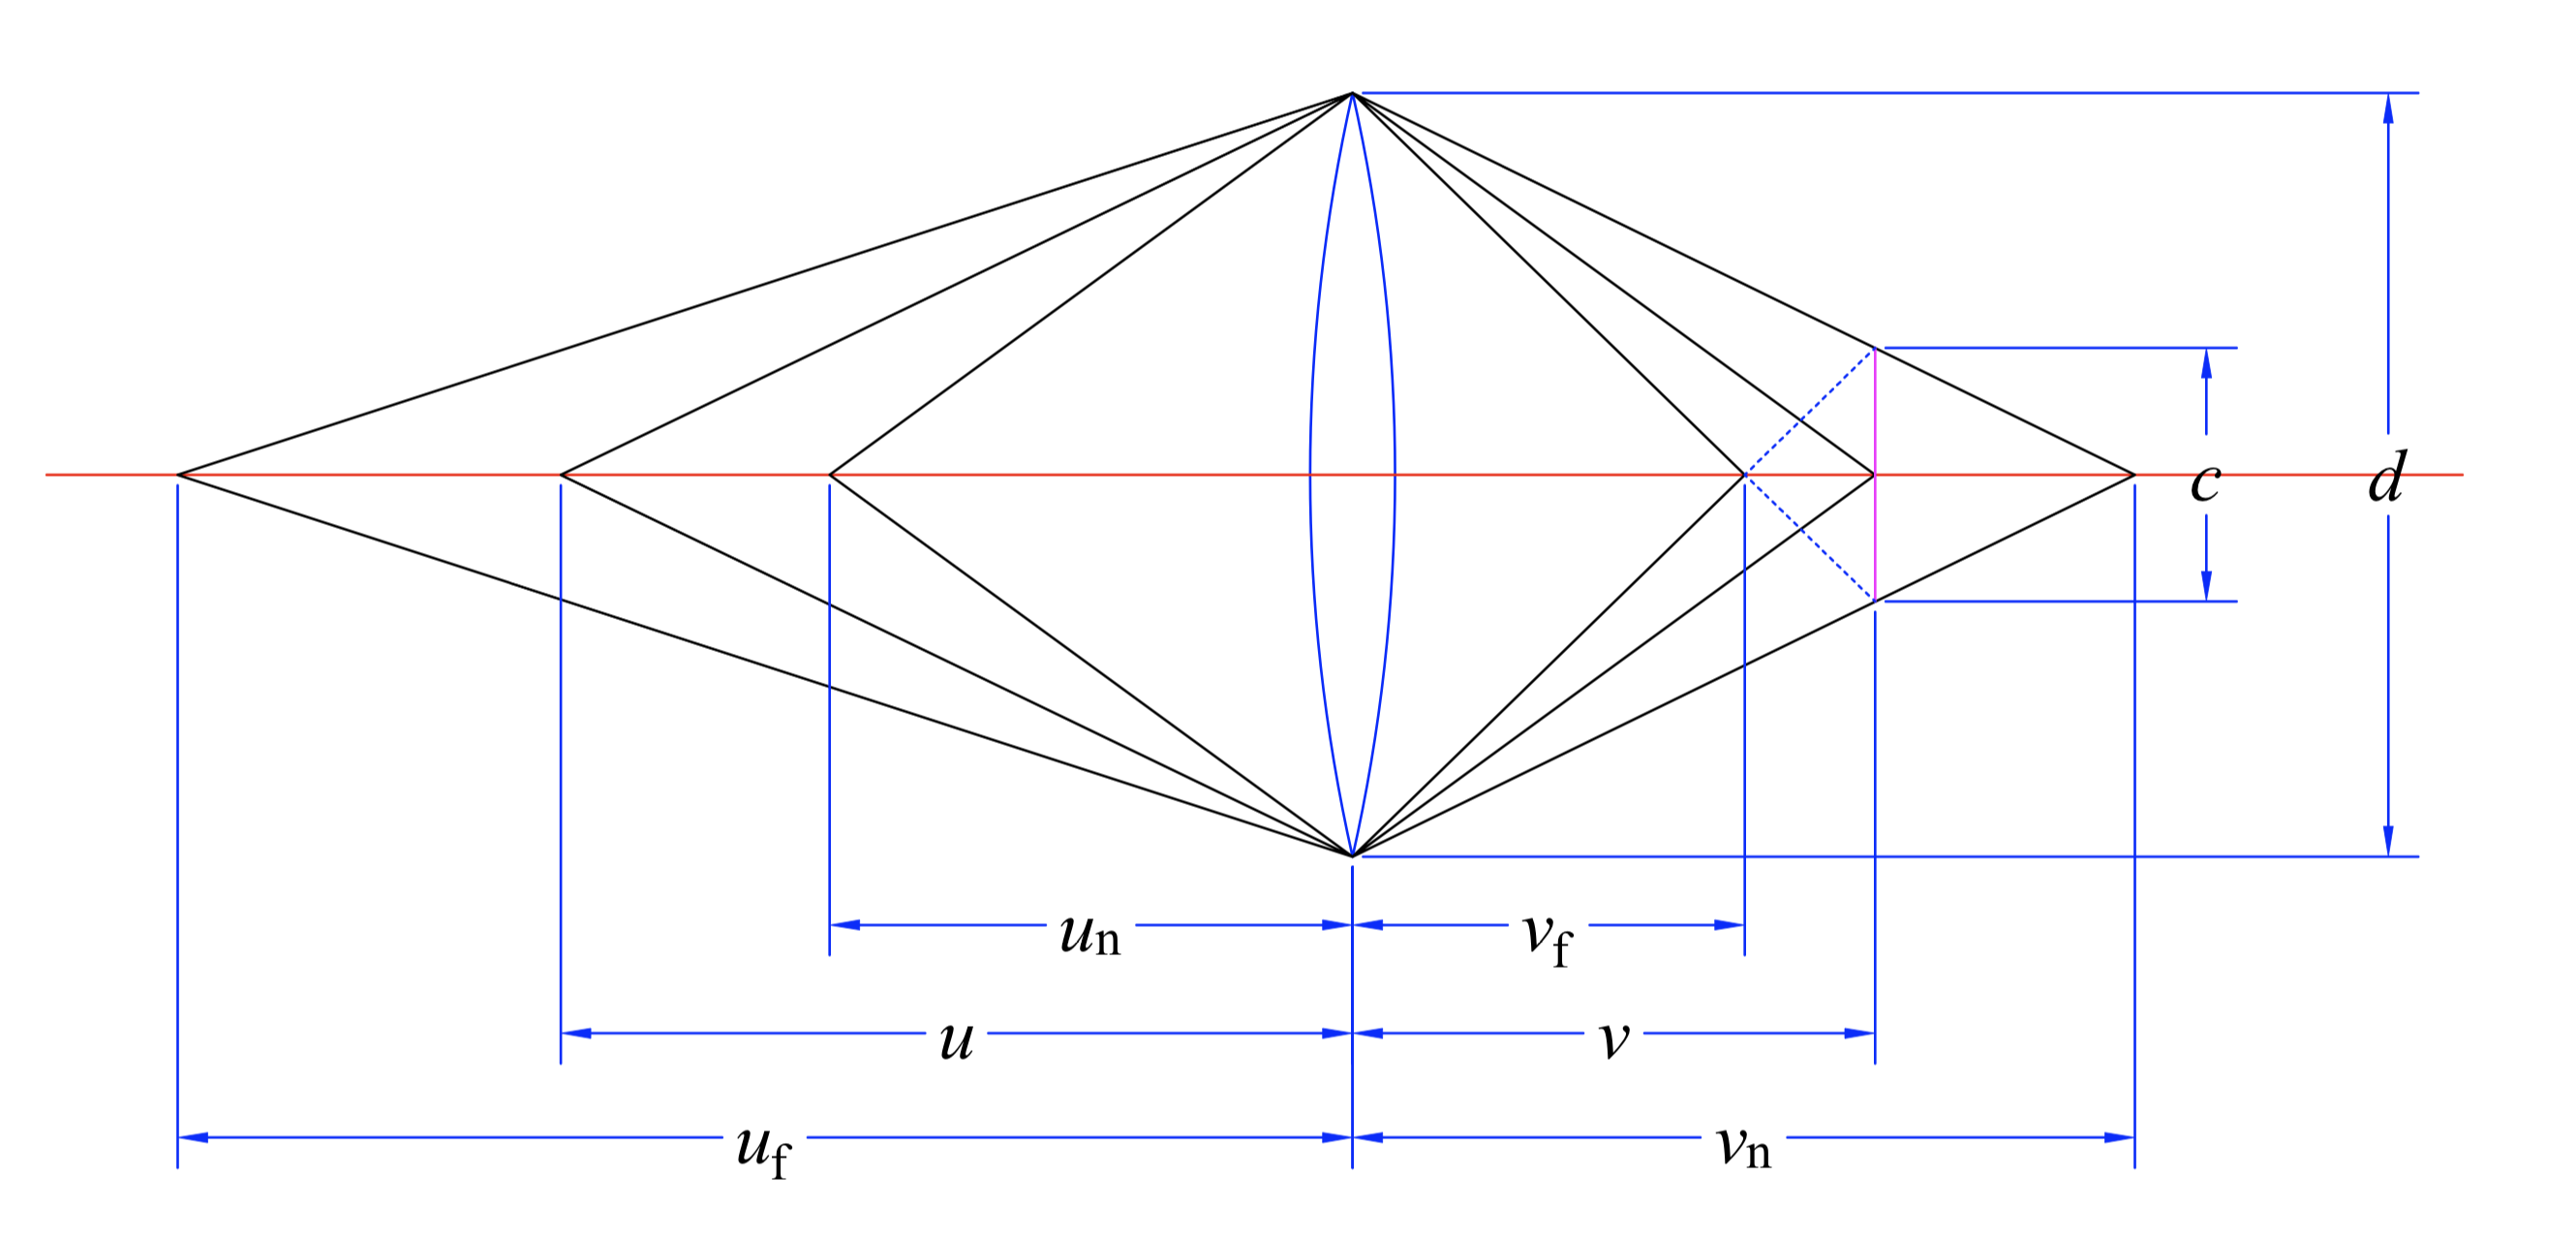
\includegraphics[width=\linewidth]{figure/fig_dofd_1} 
   \caption{DoF for Symmetrical Lens}
   \label{fig:symlens}
\end{figure}
%%% Figure 1. DoF for Symmetrical Lens

A symmetrical lens is illustrated in Figure~\ref{fig:symlens}. The object at distance $u$ is in focus at image distance $v$. The objects at distances $u_\mathrm{f}$ and $u_\mathrm{n}$ would be in focus at image distances $v_\mathrm{f}$ and $v_\mathrm{n}$, respectively; at image distance $v$, they are imaged as blur spots. The depth of field is controlled by the aperture stop diameter $d$. When the blur spot diameter is equal to the acceptable circle of confusion $c$, the near and far limits of DoF are at $u_\mathrm{n}$ and $u_\mathrm{f}$. From similar triangles,
\begin{equation}
  \frac{v_\mathrm{n} - v}{v_\mathrm{n}} = \frac c d
  % #1
  \label{eq:vni}
\end{equation}
and
\begin{equation}
  \frac{v - v_\mathrm{f}}{v_\mathrm{f}} = \frac c d
  % #2
  \label{eq:vfi}
\end{equation}
It usually is more convenient to work with the lens $f$-number than the aperture diameter; the
 $f$-number $N$ is related to the lens focal length $f$ and the aperture diameter $d$ by 
 \begin{equation}
   N=\frac f d\quad ;
   \label{eq:N}
\end{equation}
  substituting into Eqs.~\ref{eq:vni} and \ref{eq:vfi} and rearranging gives
\begin{equation}
    v_\mathrm{n}=\frac{fv}{f -N c}
   % #3
  \label{eq:vn}
\end{equation}
\begin{equation}
    v_\mathrm{f}=\frac{fv}{f + N\!c}
   % #4
  \label{eq:vf}
\end{equation}
The image distance $v$ is related to the object distance $u$ by the thin-lens equation
\begin{equation}
   \frac1u+\frac1v=\frac1f
   % #5
   \label{eq:thinlens}
\end{equation}
Rearranging into the form 
 \begin{equation}
v=\frac{uf}{u-f}\quad,
\end{equation}
substituting into Eqs.~\ref{eq:vn} and \ref{eq:vf}, and rearranging yields the corresponding relations in object space:

\begin{eqnarray}
u_\mathrm{n}&=&\frac{uf^2}{f^2 + N\!c(u-f)}\label{eq:un:os}\\
u_\mathrm{f}&=&\frac{uf^2}{f^2 - N\!c(u-f)}\label{eq:uf:os}
   % # 6,7
   \label{eq:unf}
\end{eqnarray}

Image magnification is given by\footnote{Following optical convention, this quantity would be negative to indicate an inverted image. In photography, the sign usually is omitted.}
\begin{equation}
      m=\frac v u
   % # 8
   \label{eq:mvu}
\end{equation}
Combining with Eq.~\ref{eq:thinlens} and rearranging gives
\begin{equation}
   \label{eq:m-rel1}
   u-f = \frac f m
\end{equation}
 Using that substitution and rearranging, Eqs.~\ref{eq:un:os} and \ref{eq:uf:os} can be expressed in terms of magnification as
\begin{equation}
      u_\mathrm{n}=\frac u{1+\frac{NC}{fm}}
   % # 9
   \label{eq:un2}
\end{equation}
and
\begin{equation}
      u_\mathrm{f}=\frac u{1-\frac{NC}{fm}}
         % # 10
   \label{eq:uf2}
\end{equation}

\subsection{Hyperfocal Distance}

Setting the far limit of DoF in Eq.~\ref{eq:uf:os} to infinity and solving for object distance gives
\begin{equation}
   u_\mathrm{h} = \frac{f^2}{N\!c}+f
   \label{eq:uhx}
   % #11
\end{equation}
The distance $u_\mathrm{h}$ is called the \emph{hyperfocal distance}. At the hyperfocal distance, a difference of
one focal length is insignificant, so Eq.~\ref{eq:uhx} often is given simply as
\begin{equation}
  u_\mathrm{h} \approx \frac{f^2}{N\!c}
  \label{eq:uhapprox}
  % #12
\end{equation}
When the object distance is the hyperfocal distance, the near limit of DoF, from Eq.~\ref{eq:un:os}, is 
\begin{equation}
u_\mathrm{n} = \frac{\frac{f^2}{N\!c}+f}2 = \frac{u_\mathrm{h}}2
\end{equation}
so the depth of field extends from half the hyperfocal distance to infinity. From Eq.~\ref{eq:uhx}  and the relationship (see Eq.~\ref{eq:m-rel1})
\begin{equation}
   m = \frac f{u-f}\quad,
   \label{eq:m-rel2}
\end{equation}
the magnification at $u_\mathrm{h}$ is
\begin{equation}
   m_\mathrm{h} = \frac{N\!c}f\quad.
\end{equation}
If the near limit $u_\mathrm{n}$ of DoF is fixed,  set focus to
\begin{equation}
   u = 2 u_\mathrm{n}\quad ,
   \label{eq:unearfix}
   % #15
\end{equation}
and the $f$-number to
\begin{equation}
  N\approx \frac{f^2}{2cu_\mathrm{n}}\quad .
   \label{eq:unearfix}
   % #16
\end{equation}

\subsection{Front and Rear Depth of Field}

The DoF in front of the focused object is
\begin{equation}
   u-u_\mathrm{n} = \frac{N\!cu(u-f)}{f^2 +N\!c(u-f)}
   \label{eq:17}
   % #17
\end{equation}
The DoF beyond the focused object is
\begin{equation}
u_\mathrm{f} - u = \frac{N\!cu(u-f)}{f^2 - N\!c(u-f)}
\end{equation}
The front and rear DoF can be expressed in terms of the magnification by making the substitution Eq.~\ref{eq:m-rel1}
%% u−f&f m %%% state explicitely???
into the equations for front and rear DoF and rearranging, the near DoF is
\begin{equation}
   u-u_\mathrm{n} = \frac{N\!c(1+m)}{m^2\left(1+\frac{N\!c}{fm}\right)}
   \label{eq:19}
   % #19
\end{equation}
and the far DoF is
\begin{equation}
u_\mathrm{f} - u = \frac{N\!c(1+m)}{m^2\left(1-\frac{N\!c}{fm}\right)}
   \label{eq:20}
   % #20
\end{equation}
The front:rear DoF ratio is
\begin{equation}
   \frac{u-u_\mathrm{n}}{u_\mathrm{f}-u}=\frac{f^2-N\!c(u-f)}{f^2+N\!c(u-f)} = \frac{fm-N\!c}{fm+N\!c}
   \label{eq:frrat}
   % #21
\end{equation}

It often is stated that approximately 1⁄3 of the DoF is in front of the point of focus, and 2⁄3 of
the DoF is behind it. However, this is true only at one object distance: 
\begin{equation}
u=\frac{f^2}{3N\!c} + f
\end{equation}
or slightly greater than 1⁄3 the hyperfocal distance. The front:rear DoF ratio is zero at the hyperfocal distance and beyond (the rear DoF is infinite); at high magnification, front and rear DoF are nearly equal.

\subsection{Total Depth of Field}

The total depth of field between the near and far limits is
%% (21)
\begin{eqnarray}
     u_\mathrm{f}-u_\mathrm{n} &=& \frac{uf^2 \left[f^2 +N\!c(u- f)- f^2 +N\!c(u-f)\right]}{\left[f^2 -N\!c(u-f)\right]\left[f^2 +N\!c(u-f)\right]}\nonumber\\
     & =& 
     \frac{ 2uN\!cf^2 (u- f)}{f^4 -N^2c^2(u-f)^2}
   % #22
   \label{eq:uf-n1}
\end{eqnarray}
Eliminating the terms in $u$ and $u - f$ by noting that 
\begin{equation}
u = \frac{m+1}m f\quad ,
\end{equation}
%% m
and
\begin{equation}
    u-f = \frac f m\quad,
\end{equation}
total depth of field in terms of magnification is
\begin{eqnarray}
u_\mathrm{f}-u_\mathrm{n} &=& \frac{2f\left(\frac{m+1}m\right)N\!cf^2\left(\frac f m\right)}{f^4 -N^2c^2\left(\frac f m\right)^2} \nonumber\\
&=& \frac{2f\left(\frac{m+1}m\right)}{\frac{fm}{N\!c}-\frac{N\!c}{fm}}
% #23
\label{eq:uf-n2}
\end{eqnarray}

At the hyperfocal distance, the two terms in the denominator are equal, and the DoF is infinite, although only objects at or beyond the near limit of DoF are rendered acceptably sharp. At distances beyond the hyperfocal distance, the calculated DoF is negative, but this has no physical significance. When the DoF is infinite, the only quantity of interest would seem to be the near limit of DoF, which, as can be seen from Eq.~\ref{eq:un2}, is closer with a lens of shorter focal length.

Multiplying the numerator and denominator of Eq.~\ref{eq:uf-n2} by $\frac{N\!cm}f$
gives
\begin{equation}
   u_\mathrm{f}-u_\mathrm{n} = \frac{2N\!c(m+1)}{m^2-\left(\frac{N\!c}f\right)^2}
   % #24
      \label{eq:uf-n3}
\end{equation}
It can be seen from Eq.~\ref{eq:uf-n3} that a shorter focal length
gives a greater DoF. When $u \ll u_\mathrm{h}$, the second term in the denominator is small compared with the first, so that
\begin{equation}
   u_\mathrm{f}-u_\mathrm{n} \approx 2N\!c\frac{m+1}{m^2}
   % #25
   \label{eq:uf-n4}
\end{equation}
and the DoF is independent of focal length.

Note that for constant DoF in Eq.~\ref{eq:uf-n4}, there is a reciprocal relationship between $N$ and
$c$: using a greater $f$-number is equivalent to specifying a smaller circle of confusion, and vice versa. This can be useful when using lens DoF scales that assume a final-image enlargement different from that actually intended. For example, if the lens DoF scales assume a 5× enlargement, and the image actually requires 7× enlargement, using an $f$-number one step greater (e.\,g., \f 8 rather than \f{5.6}) will effectively reduce the CoC by a factor of $\sqrt 2$ , sufficient to compensate for the greater enlargement.
\subsection{Focus and Minimum $f$-Number for Given Depth of Field}

If the depth of field is to extend to infinity, the minimum $f$-number
is obtained by setting the focus to the hyperfocal distance. Many
images, however, do not require that the DoF extend to infinity. To
have the DoF between two arbitrary distances $u_\mathrm{n}$ and $u_\mathrm{f}$, Eqs. (6)
and (7) can be solved for $N$, combined, and solved for the object
distance $u$ to give
\begin{equation}
  \label{eq:u}
  u = \frac{2u_\mathrm{f}u_\mathrm{n}}{u_\mathrm{f}+u_\mathrm{n}}
  % #26
\end{equation}
the \emph{harmonic mean} of the near and far distances. Note that the distance is independent of $N$: if the $f$-number is increased to decrease the effective CoC, there is no need to refocus.

The required $f$-number is obtained by solving Eqs. (6) and (7) for
$u$, combining, and solving for $N$, giving
\begin{equation}
  \label{eq:N}
  N = \frac{f^2}c\frac{u_\mathrm{f} - u_\mathrm{n}}{u_\mathrm{f}(u_\mathrm{n}-f)+u_\mathrm{n}(u_\mathrm{f}-f)}
\end{equation}

If the near and far limits of DoF are large in comparison with the lens focal length,
\begin{equation}
  \label{eq:Napprox}
  N\approx \frac{f^2}c\frac{u_\mathrm{f} - u_\mathrm{n}}{2u_\mathrm{f}u_\mathrm{n}}
  % #28
\end{equation}
If the focus is set using Eq.~(\ref{eq:u}), the DoF in front of the
focus point is
\begin{equation}
  \label{eq:DOFf}
  u-u_\mathrm{n}=\frac{2u_\mathrm{n}u_\mathrm{f}-u_\mathrm{n}u_\mathrm{f}-u_\mathrm{n}^2}{u_\mathrm{n} + u_\mathrm{f}} = \frac{u_\mathrm{n}(u_\mathrm{f} - u_\mathrm{n})}{u_\mathrm{n} + u_\mathrm{f}}
\end{equation}
and the DoF beyond the focus point is
\begin{equation}
  \label{eq:DOFb}
  u_\mathrm{f} - u = \frac{u_\mathrm{f}^2 +u_\mathrm{n}u_\mathrm{f}-2u_\mathrm{n}u_\mathrm{f}}{u_\mathrm{n} + u_\mathrm{f}} = \frac{u_\mathrm{f}(u_\mathrm{f} - u_\mathrm{n})}{u_\mathrm{n} + u_\mathrm{f}}
\end{equation}
The front:rear DoF ratio then is
\begin{equation}
  \label{eq:frrat}
  \frac{u - u_\mathrm{n}}{u_\mathrm{f} - u} = \frac{u_\mathrm{n}}{u_\mathrm{f}}
  % #29
\end{equation}
Except when the near and far limits of DoF coincide, the focus point always is closer to the
near limit. The near-to-total ratio is 1⁄3 only when $u_\mathrm{f} = 2u_\mathrm{n}$.

\subsection{Image-Side Relationships}
Most discussions of depth of field concentrate on the object side of the lens; in practice, however, camera settings usually are determined using image distances, whether directly in the case of a view camera, or by using distance and DoF scales on hand-camera lenses. With a view camera, the image distances are obtained by focusing on objects at the desired near and far limits of DoF, and noting the lens extension in each case. The image distances $v_\mathrm{n}$ and $v_\mathrm{f}$ correspond to object distances $u_\mathrm{n}$ and $u_\mathrm{f}$; the difference $v_\mathrm{n}-v_\mathrm{f}$ between the near and far image distances is the \emph{focus spread} $\Dv$.

Combining Eqs. (1) and (2) gives the image distance $v$ that will set
the DoF between object distances $u_\mathrm{n}$ and $u_\mathrm{f}$:
\begin{equation}
  \label{eq:v}
  v =  \frac{2v_\mathrm{n}v_\mathrm{f}}{v_\mathrm{n}+v_\mathrm{f}}
  % #30
\end{equation}
the harmonic mean of the near and far image distances. The harmonic mean always is less than the arithmetic mean, but when the focus spread is small, the harmonic mean and arithmetic mean are nearly equal, so that
\begin{equation}
  \label{eq:vapprox1}
  v\approx\frac{v_\mathrm{n}+v_\mathrm{f}}2
  % #31
\end{equation}
or
\begin{equation}
  \label{eq:vapprox2}
  v \approx v_\mathrm{f} + \frac \Dv 2
  % #32
\end{equation}
Again combining Eqs. (1) and (2), the far:near distribution of the focus spread is
\begin{equation}
   \frac{v-v_\mathrm{f}}{v_\mathrm{n}-v} = \frac{v_\mathrm{f}}{v_\mathrm{n}}\quad.
   \label{eq:33}
   % #33
\end{equation}
Using Eq. (5) to substitute for $v_\mathrm{n}$ and $v_\mathrm{f}$, and then rearranging, the focus spread in terms   the object distances is
\begin{equation}
   v_\mathrm{n}-v_\mathrm{f} = \frac{(u_\mathrm{f}-u_\mathrm{n})f^2}{(u_\mathrm{f}-f)(u_\mathrm{n}-f)}
\end{equation}
or
\begin{equation}
   \Dv \approx (u_\mathrm{f} - u_\mathrm{n})m_\mathrm{n}m_\mathrm{f} \quad.
   \label{eq:34}
   % #34
\end{equation}

For different camera formats, if the perspective and framing are held constant by suitable choice of lenses, the magnifications of the near and far objects are proportional to the format size. Consequently, the focus spread is proportional to the square of the format size, so that a focus spread of 0.5\,mm in 35\,mm format corresponds to focus spreads of 8\,mm in 4$\times$5 and 32\,mm in 8$\times$10.

Except when the focus spread is zero, the exact focus distance v always will be slightly closer to the far image distance. In most cases, the approximate focus setting is close to the exact value; the difference is given by
\begin{equation}
v_\mathrm{ap} - v =  \frac{v_\mathrm{n}+v_\mathrm{f}}2 - \frac{2v_\mathrm{n}v_\mathrm{f}}{v_\mathrm{n} + v_\mathrm{f}} = \frac{v_\mathrm{n}^2+2v_\mathrm{n}v_\mathrm{f}+v_\mathrm{f}^2-4v_\mathrm{n}v_\mathrm{f}}{2(v_\mathrm{n}+v_\mathrm{f})} = \frac{(v_\mathrm{n} - v_\mathrm{f})^2}{2(v_\mathrm{n}+v_\mathrm{f})} 
   \label{eq:35}
   % #35
\end{equation}
The difference between the approximate and exact values is proportional to the square of the focus spread, and for a given focus spread, is greatest at distant focus. In all cases,
\begin{equation}
v_\mathrm{ap} - v \leq \frac{(v_\mathrm{n} - v_\mathrm{f})^2}{4f} 
\end{equation}
This difference always is a positive quantity, so that the image distance determined with the approximate formula always will be slightly greater than that determined with the exact formula, and accordingly, focus will be slightly closer than optimum. Evens (2003) describes this relationship in a slightly different but equivalent form.

With focus set by Eq. (30), the required $f$-number is
\begin{equation}
    N = \frac f c\frac{v_\mathrm{n}-v_\mathrm{f}}{v_\mathrm{n}+v_\mathrm{f}}
    \label{eq:36}
    % #36
\end{equation}
When the focus spread is small, $v_\mathrm{n} + v_\mathrm{f} \approx 2v$, and
\begin{equation}
   N \approx \frac f v \frac\Dv{2c}
   \label{eq:37}
   % #37
\end{equation}
It sometimes is more convenient to express Eq. (37) in terms of the magnification; substituting the relation
\begin{equation}
   v=(1+m)f
\end{equation}
into Eq. (37), giving
\begin{equation}
   N\approx\frac1{1+m}\frac\Dv{2c}
   \label{eq:38}
   % #38
\end{equation}

Except at close working distances, $m$ is small, and Eq. (38) often can be simplified to 
\begin{equation}
N\approx\frac\Dv{2c}
   \label{eq:39}
   % #39
\end{equation}
When this is done, the ratio of approximate to exact $f$-number is
\begin{equation}
    \frac{N_\mathrm{ap}}N = \frac{v_\mathrm{n}-v_\mathrm{f}}{2c}\frac c f\frac{v_\mathrm{n}+v_\mathrm{f}}{v_\mathrm{n}-v_\mathrm{f}} = \frac{v_\mathrm{n}+v_\mathrm{f}}{2f}\approx\frac v f = 1+m
    \label{eq:40}
    %. #40
\end{equation}

The error increases with image distance, or equivalently, with magnification. Eq. (39) gives a greater $f$-number than actually required, so to use it is to err on the conservative side. If this error is unacceptable, Eq. (37) or (38) can be used for closeup work.

Equations (32) and (39) are well known to many view camera users; the rear standard is set to a position halfway between the points of focus for the near and far objects, and the lens $f$-number is calculated from the focus spread. Although Eqs. (30) and (36) are simple enough, especially if the calculations are done with a programmable calculator or handheld computer, they require the absolute image distances $v_\mathrm{n}$ and $v_\mathrm{f}$, which often are not easy to determine, especially if camera movements are employed. Eqs. (32) and (39) require only the difference between the near and far image distances, which usually is easily measured; consequently, these equations are the ones most commonly used on hand-camera lens DoF scales and on DoF calculators for view cameras. Eqs (37) and (38) require the absolute image distance, but a reasonable estimate of image distance or of the magnification often will suffice. It can be shown that Eqs. (32) and (39) are valid even if swings and tilts are employed.

If the camera does not include a DoF calculator, measurement of focus spread is much easier if the bed or focusing rail includes a scale, and measurements can be more precise if the focusing knob includes an additional scale. See Hayashi for a description of adding a Sinar-type DoF scale to the focusing knob, and Evens (2003) for a discussion of adding scales to both the rail and the knob.

On a hand camera, the lens DoF scales usually implement these same formulae. With autofocus lenses, however, there may be no easy means of controlling DoF; the distance-scale markings usually are widely spaced, and the DoF scales, if even provided, usually are so small that using them to determine focus and $f$-number is all but impossible. Although the benefits of autofocus are undeniable, an unfortunate consequence is that even the most advanced autofocus 35\,mm cameras cannot perform a task that was easily accomplished with the most basic manual-focus cameras.\footnote{When Canon introduced autofocus cameras, many of the bodies included a feature, Depth-of-Field Automatic Exposure, that functioned in much the same manner as DoF scales on manual-focus lenses. Unfortunately, this feature was eliminated from new models introduced since early 2004.}

If lens DoF scales are not available, and it is impractical to measure image distances, Eqs. (26) and (28) can be used if there is a convenient way to measure object distances. With a suitable external rangefinder, these formulae could provide a means of controlling DoF with autofocus lenses.

Substituting Eq. (5) into Eq. (11) and rearranging gives the image distance $v_\mathrm{h}$ corresponding to the hyperfocal distance $u_\mathrm{h}$:
\begin{equation}
   v_\mathrm{h} = f + N\!c
   % # (41)
   \label{eq:vh} 
\end{equation}
%% 
This image distance will put the DoF between half the hyperfocal distance and infinity, and
can be useful when designing a fixed-focus camera.

\subsection{Depth of Field and Background Blur vs. Focal Length}

Recall that the CoC is the diameter of the blur spot at the near and far limits of DoF; the diameter of the blur spot for a point on a defocused object at an arbitrary distance is obtained by solving Eqs. (6) and (7) for $c$, and replacing the near and far distances by $u_\mathrm{d}$, leading to
\begin{equation}
   k = \frac1N \frac{f^2}{u-f}  \frac{|u_\mathrm{d} - u|}{u_\mathrm{d}} = \frac{fm}N \frac{|u_\mathrm{d} - u|}{u_\mathrm{d}}
   % # 42
   \label{eq:k1}
\end{equation}
Equivalently, for a point at a distance $x_\mathrm{d}$ from the plane of focus, 
\begin{equation}
   k = \frac{fm}N \frac{x_\mathrm{d}}{u\pm x_\mathrm{d}}
   % # 43
   \label{eq:k2}
\end{equation}
 The sign in the denominator is negative when the defocused object is in front of the focused object.

For constant magnification of the focused object, the diameter of the blur spot increases with lens focal length; however, the magnification of the defocused object also increases with focal length. The most appropriate measure of “background blur” may be the diameter of the blur spot relative to the image size of the defocused object. Image size is proportional to the magnification; the magnification $m_\mathrm{d}$ of an object at a distance xd from the plane of focus is
\begin{equation}
   m_\mathrm{d} = \frac v {u_\mathrm{d}} = \frac{(m+1)f}{u_\mathrm{d}} 
   % # (44) 
   \label{eq:md}
\end{equation}
%% 
If the “relative blur” $k_\mathrm{r}$ is the ratio of blur spot diameter to magnification, then
\begin{equation}
    \frac{k}{m_\mathrm{d}} = \frac m{m+1}\frac{|x_\mathrm{d}|}N
    % #45
    \label{eq:km}
\end{equation}

It often is claimed that a long-focus lens gives less DoF and more background blur than a short-focus lens. However, Eq. (25) shows that, when the object distance is small in comparison with the hyperfocal distance, DoF is independent of focal length, and Eq. (45) shows that the “relative blur” is independent of focal length at all distances. However, if the defocused object is sufficiently distant, it may appear so small with a short-focus lens that the blurring is not obvious; in such a case, the long-focus lens may give subjectively greater background blur. The perspective with a long-focus lens will, of course, be different from the perspective with a short-focus lens.

Van Walree (2002) gives an excellent description and illustration of this behavior in slightly different terms.

\section{Different Circles of Confusion for Near and Far Limits of Depth of Field}

The conventional approach to DoF is based on distinguishing a point from a blur spot in the image, and uses equal CoCs for the near and far limits. Although the CoC usually is quite small in comparison with the imaged size of near objects, it can be quite large in comparison with the imaged size of distant objects, in some cases so much so that a distant object becomes unrecognizable. Although many undoubtedly would maintain that, under normal viewing conditions, a blur spot either is distinguishable from a point or it is not, others (Merklinger 1992; Englander 1994) maintain that sharpness perception is context dependent, and that greater sharpness is required in distant objects to give an acceptably sharp image. This requirement can be addressed by using a smaller CoC for the far limit of DoF; in some respects, this approach is similar to the concept of “relative blur.”

\subsection{Image-Side Relationships}

Eqs. (1) and (2) assumed identical CoCs for the near and far limits of DoF; using different near and far values $c_\mathrm{n}$ and $c_\mathrm{f}$, we have
\begin{equation}
   \frac{v_\mathrm{n} - v}{v_\mathrm{n}} = \frac{c_\mathrm{n}}d\hphantom{\quad.}
   \label{eq:46}
   % #46
\end{equation}
and
\begin{equation}
   \frac{v - v_\mathrm{f}}{v_\mathrm{f}} = \frac{c_\mathrm{f}}d \quad .
   \label{eq:47}
   % #47
\end{equation}
Replacing $d$ with the focal length and $f$-number gives
\begin{equation}
   \frac{v_\mathrm{n} - v}{v_\mathrm{n}} = \frac{N\!c_\mathrm{n}}f\hphantom{\quad.}
   \label{eq:48}
   % #48
\end{equation}
and
\begin{equation}
   \frac{v - v_\mathrm{f}}{v_\mathrm{f}} = \frac{N\!c_\mathrm{f}}f \quad .
   \label{eq:49}
   % #49
\end{equation}
Combining Eqs. (48) and (49) and solving for $v$ gives
\begin{equation}
v = \frac{(c_\mathrm{n} + c_\mathrm{f}) v_\mathrm{n} v_\mathrm{f}}{c_\mathrm{n}v_\mathrm{v} + c_\mathrm{f}v_\mathrm{f}}
   \label{eq:50}
   % #50
\end{equation}
Again combining Eqs. (48) and (49), the far:near distribution of the focus spread is
\begin{equation}
   \frac{v - v_\mathrm{f}}{v_\mathrm{n} - v} = \frac{c_\mathrm{f}v_\mathrm{f}}{c_\mathrm{n}v_\mathrm{n}}
   \label{eq:51}
   % #51
\end{equation}
Unless the focus spread is large, we usually can take $v_\mathrm{f} \approx v_\mathrm{n}$ on the right-hand side of
 Eq. (51), so that
\begin{equation}
   \frac{v - v_\mathrm{f}}{v_\mathrm{n} - v} \approx \frac{c_\mathrm{f}}{c_\mathrm{n}}
   \label{eq:52}
   % #52
\end{equation}
Rearranging and solving for $v$ gives
\begin{equation}
   v\approx{c_\mathrm{f}v_\mathrm{n}+c_\mathrm{n}v_\mathrm{f}}{c_\mathrm{n}+c_\mathrm{f}}
   \label{eq:53}
   % #53
\end{equation}
or
\begin{equation}
   v\approx v_\mathrm{f}+\frac{c_\mathrm{f}}{c_\mathrm{n}+c_\mathrm{f}}\Dv
   \label{eq:54}
   % #54
\end{equation}
where $Δv$ is the focus spread $v_\mathrm{n} - v_\mathrm{f}$. Combining Eqs. (48) and (49) and solving for $N$ gives
\begin{equation}
   N=\frac{(v_\mathrm{n}-v_\mathrm{f})f}{c_\mathrm{n}v_\mathrm{n}+c_\mathrm{f}v_\mathrm{f}}
   \label{eq:55}
   % #55
\end{equation}

%% N & (vn - vf ) f (55) cnvn +cfvf
To within sufficient accuracy for determining $N$, we usually can take $v_\mathrm{n} \approx v_\mathrm{f} \approx v$ in the denominator, so that
\begin{equation}
   N\approx\frac f v \frac{v_\mathrm{n}-v_\mathrm{f}}{c_\mathrm{n}+c_\mathrm{f}}
   \label{eq:56}
   % #56
\end{equation}
Except for closeup work, it usually is acceptable to take $v \approx f$, so that Eq. (56) further simplifies to
\begin{equation}
   N\approx\frac \Dv{c_\mathrm{n}+c_\mathrm{f}}
   \label{eq:57}
   % #57
\end{equation}
Assuming that $c_\mathrm{f} < c_\mathrm{n}$, Eq. (54) gives an image distance closer to the far image distance than does Eq. (32), and Eq. (57) gives a greater $f$-number than does Eq. (39).

Englander (1994) suggested, in effect, that when the DoF extends to infinity, $c_\mathrm{f}$ should be $1⁄2 c_\mathrm{n}$. From Eq. (54), focus then would be set to
\begin{equation}
  v = v_f + \frac 1 3 \Dv\quad,
  \label{eq:57+}
\end{equation}
and from Eq. (57), the $f$-number would be
\begin{equation}
  N = \frac\Dv{1.5c\mathrm{n}}\quad,
  \label{eq:57++}
\end{equation}
or approximately 0.83 step greater than would result from equal near
and far CoCs. Merklinger (1992) desired greater sharpness in distant
objects, and suggested\footnote{Merklinger actually suggested 1⁄30\,mm
  for the near-limit CoC; 0.025\,mm is used here for consistency with
  the other examples.} a far-limit CoC of 1⁄150\,mm for 35\,mm film;
using 0.025\,mm for the near-limit CoC, $c_\mathrm{f} \approx 1⁄4 c_\mathrm{n}$. From
Eq. (54), focus would be set to
\begin{equation}
  \label{eq:57+++}
  v=v_\mathrm{f}+\frac15\Dv\quad,
\end{equation}
and from Eq. (57), the $f$-number would be
\begin{equation}
  \label{eq:57++++}
  N=\frac \Dv{1.25c_\mathrm{n}}\quad ,
\end{equation}
or approximately 1\,1⁄3 steps greater than would result from equal near and far CoCs. If the CoC were to be reduced by a factor of four simply by stopping down without refocusing, the $f$-number would need to increase by a factor of four, or four steps. Of course, the latter approach would decrease the CoC for both near and far objects; in some situations, this might be of value, in others it might not.

\subsection{Object-Side Relationships}
\label{sec:object-side-relat}


The object-side equations for distance and $f$-number are obtained by
substituting the conjugate relationship
\begin{equation}
  \label{eq:57+++++}
  v=\frac{uf}{u-f}
\end{equation}
into Eqs. (50) and (55), giving
\begin{equation}
  \label{eq:58}
  u = \frac{(c_\mathrm{n}+c_\mathrm{f})u_\mathrm{n}u_\mathrm{f}}{c_\mathrm{n}u_\mathrm{n}+c_\mathrm{f}u_\mathrm{f}}
   % #58
\end{equation}
and
\begin{equation}
  \label{eq:59}
  N=\frac{(u_\mathrm{f}-u_\mathrm{n})f^2}{c_\mathrm{n}u_\mathrm{n}(u_\mathrm{f}-f)+c_\mathrm{f}u_\mathrm{f}(u_\mathrm{n}-f)}
  %  #59
\end{equation}
If the near and far distances are large in comparison with the lens
focal length,
\begin{equation}
  \label{eq:1}
  N\approx\frac{(u_\mathrm{f}-u_\mathrm{n})f^2}{(c_\mathrm{n}+c_\mathrm{f})u_\mathrm{n}u_\mathrm{f}}
\end{equation}
The near and far limits of DoF are obtained by substituting  into
Eqs. (48) and (49), giving
\begin{equation}
  \label{eq:61}
  u_\mathrm{n}=\frac{uf^2}{f^2+N\!c_\mathrm{n}(u-f)}\hphantom{\quad.}
  % #61
\end{equation}
and
\begin{equation}
  \label{eq:62}
  u_\mathrm{f}=\frac{uf^2}{f^2-N\!c_\mathrm{f}(u-f)}\quad.
  % #61
\end{equation}
Setting the far limit of DoF to infinity and solving for object
distance gives
\begin{equation}
  \label{eq:uh}
  u_\mathrm{h}=\frac{f^2}{N\!c_\mathrm{f}}+f
  % #63
\end{equation}
the hyperfocal distance for different near- and far-limit CoCs. When
the object distance is the hyperfocal distance, the near limit of DoF,
from Eq. (61), is
\begin{equation}
  \label{eq:un}
  u_\mathrm{n} = \frac{c_\mathrm{f}}{c_\mathrm{n}+c_\mathrm{f}}\left(\frac{f^2}{N\!c_\mathrm{f}}+f\right)
  % #64
\end{equation}

\section{The Object Field Method}
\label{sec:object-field-method}


Sometimes the recognizability of objects may be more important than a specified sharpness in the image; this long has been the case in aerial surveillance photography; see Williams (1990) for a discussion of “ground resolution.” The objects of interest in aerial surveillance essentially are at infinity; Merklinger’s Object Field Method applied the same criterion to objects throughout the image.

Generally, an object is recognizable if key features are reproduced at a size equal to or larger than the size of the blur spot. The expressions on the object side to ensure this reproduction are straightforward; when the same resolution criteria apply at near and far distances, the focus distance is
\begin{equation}
   u=\frac{u_\mathrm{n}+u_\mathrm{f}}2
   \label{eq:65}
   % #65
\end{equation}
and the $f$-number is
\begin{equation}
   N = \frac{u_\mathrm{f} - u_\mathrm{n}}{u_\mathrm{n}+u_\mathrm{f}}\frac f S
   \label{eq:66}
   % #66
\end{equation}
where $S$ is the size of the smallest feature to be resolved.

Eqs. (65) and (66) are simple to apply when an easy means of determining object
distance is available, such as with manual-focus hand-camera lenses that have readable distance scales, or perhaps with a laser rangefinder. However, the expressions on the image side are more complex. Merklinger’s resolution criteria derive strictly from consideration of object features, but the effect essentially is equivalent to using different CoCs for near and far objects. This again is similar to the concept of “relative blur.” When the same resolution criteria apply at near and far distances, the near and far CoCs are proportional to their relative magnifications:
\begin{equation}
   \frac{c_\mathrm{f}}{c_\mathrm{n}}=\frac{m_\mathrm{f}}{m_\mathrm{n}}
   \label{eq:67}
   % #67
\end{equation}
\begin{equation}
   m_\mathrm{x} = \frac v {u_\mathrm{x}} = \frac v {v_\mathrm{x}} \frac{v_\mathrm{x} - f}f
   \label{eq:67+}
\end{equation}
for the near and far magnifications gives
\begin{equation}
   \frac{c_\mathrm{f}}{c_\mathrm{n}} = \frac{v_\mathrm{n}}{v_\mathrm{n}} \frac{v_\mathrm{f} - f}{v_\mathrm{n} - f}
   \label{eq:68}
   % #68
\end{equation}
The expressions for focus distance and $f$-number do not lend themselves to easily used simplifications, except when the far limit of DoF extends to infinity: then $v_\mathrm{f} = f$, and $c_\mathrm{f} = 0$. From Eq. (54), the focus is set to infinity; from Eq. (6), the near limit of DoF then is
\begin{equation}
   u_\mathrm{n} = \frac{f^2}{N\!c_\mathrm{n}}\quad,
   \label{eq:69}
   % #69
\end{equation}
essentially the hyperfocal distance. From Eq. (57), the $f$-number is
\begin{equation}
   N \approx \frac{v_\mathrm{n} - f}{c_\mathrm{n}}
   \label{eq:70}
   % #70
\end{equation}
or two steps greater than that resulting from the same near distance using equal near and far CoCs. Of course, with the Object Field Method, the absolute value of the CoC derives strictly from object features, so it may not be the same as the CoC determined with the conventional approach to DoF.

Alternatively, the $f$-number can be determined from the near object distance by rearranging Eq. (69):
\begin{equation}
   N = \frac{f^2}{c_\mathrm{n}u_\mathrm{n}}\quad,
   \label{eq:71}
   % #71
\end{equation}
Eq. (71) also indicates that the required $f$-number is twice that of the conventional method: the near limit of DoF with the conventional method is half the hyperfocal distance, and halving the distance in Eq. (71) requires doubling the $f$-number.

With a hand camera, it usually is easier to determine the $f$-number using Eq. (71) rather than Eq. (70), although with most autofocus lenses, the distance scale may be essentially unreadable unless the near distance is quite close.

For a given $f$-number, the Object Field Method gives greater sharpness to distant objects at the expense of slightly less sharpness in near objects; for a given near-limit sharpness, the greater sharpness of distant objects comes at the expense of a greater $f$-number than required with equal near and far CoCs. Although the cost of the greater distant sharpness is substantial, it nonetheless is considerably less than the cost of achieving the same sharpness simply by increasing the $f$-number without refocusing. In practice, the Object Field Method often is easiest to use with infinity focus, especially with a hand camera, for which a slightly closer focus can be difficult to set accurately.

When recognizability of objects is the most important consideration, as usually is the case in surveillance photography, the Object Field Method probably is better than the conventional method, especially if parts of the image are to be examined at high magnification to resolve small details. How much this holds true in general pictorial photography is a matter of personal taste.

\subsection{Depth of Field and Camera Format}

For two different camera formats 1 and 2, with each camera at the same object distance, and the lens focal lengths chosen to give same image framing, the $f$-numbers $N_1 $ and $N_2$ required to give the same total depth of field are, from Eq. (25),
\begin{equation}
\frac{N_2}{N_1}\approx\frac{c_1}{c_2}\frac{m_1+1}{m_2+1}\left(\frac{m_2}{m_1}\right)^2
   \label{eq:72}
   % #72
\end{equation}
When the object distance is large in comparison with the lens focal length, magnification is small, and
\begin{equation}
\frac{m_1+1}{m_2+1} \approx 1\quad,
\end{equation}
so that
\begin{equation}
\frac{N_2}{N_1}\approx\frac{c_1}{c_2}\left(\frac{m_2}{m_1}\right)^2\quad.
   \label{eq:73}
   % #73
\end{equation}
Image magnification $m$ corresponds to a characteristic dimension $l$ of the camera format, so that
\begin{equation}
\frac{m_1}{m_2} = \frac{l_1}{l_2}
   \label{eq:74}
   % #74
\end{equation}
If the final images are to be the same size, the acceptable circles of confusion $c_1$ and $c_2$ are in proportion to the format size:
%% 
%% Page 19
\begin{equation}
\frac{c_1}{c_2} = \frac{l_1}{l_2}
   \label{eq:75}
   % #75
\end{equation}
and
\begin{equation}
\frac{N_2}{N_1}\approx \frac{l_1}{l_2}  \frac{l_2^2}{l_1^2} =  \frac{l_2}{l_1}\quad.
   \label{eq:73}
   % #73
\end{equation}

If the characteristic dimension is the short dimension of the format, the ratio of the 4×5 (96\,mm × 120\,mm) and 35\,mm (24\,mm × 36\,mm) formats is 4. If a 35\,mm camera using a 75\,mm lens required \f8 at 1/250 second, a 4×5 camera using a 300\,mm lens and viewing the same object from the same camera position would require \f{32} at 1/15 second for the same depth of field. For a stationary subject, such as architecture, either combination probably would be fine, but for a moving subject, such as a field of wildflowers on a windy day, the 1/15\,sec. shutter speed might not be sufficient to prevent motion blur. Of course, just the opposite problem can arise when a shallow DoF is desired with a small-format digital sensor—the lens may not allow a sufficiently small $f$-number to give the desired effect.

For a given $f$-number, the ratio of the depths of field of the two camera formats is given by
\begin{equation}
   \frac{\mathrm{DoF}_1}{\mathrm{DoF}_2} \approx \frac{l_1}{l_2}
   \label{eq:77}
   % #77
\end{equation}

If a 35\,mm camera using a 75\,mm lens and a 4×5 camera using a 300\,mm lens were set to the same $f$-number, the image from the 35\,mm camera would have 4 times the depth of field of the image from the 4×5.

The rule that “DoF is inversely proportional to format size” is useful for describing practical results obtained with different camera formats, although the approximations used to derive it are valid only for a limited range of object distances. There is no simple expression for the valid range of distances, but in many cases (allowing about a 20\,\% error), it is between about 3 times the focal length of the lens on the smaller format, and about 1⁄2 the hyperfocal distance of the lens on the larger format.

\subsection{Depth of Field for an Asymmetrical Lens}
Most treatments of depth of field assume a symmetrical lens for which the entrance and exit pupils are the same size, and for which the pupils coincide with the object and image principal planes. Although this assumption is reasonable for most large-format lenses of short and medium focal length, it may not be appropriate for telephoto designs. For most  35\,mm and medium-format single-lens reflex cameras, the only nearly symmetrical lenses are those with focal length approximately equal to the film diagonal; longer-focus lenses usually are telephoto designs, and shorter-focus lenses are retrofocus designs that allow the rear element to clear the reflex mirror.
%% Page 20
\begin{figure}[htbp] %  figure placement: here, top, bottom, or page
   \centering
   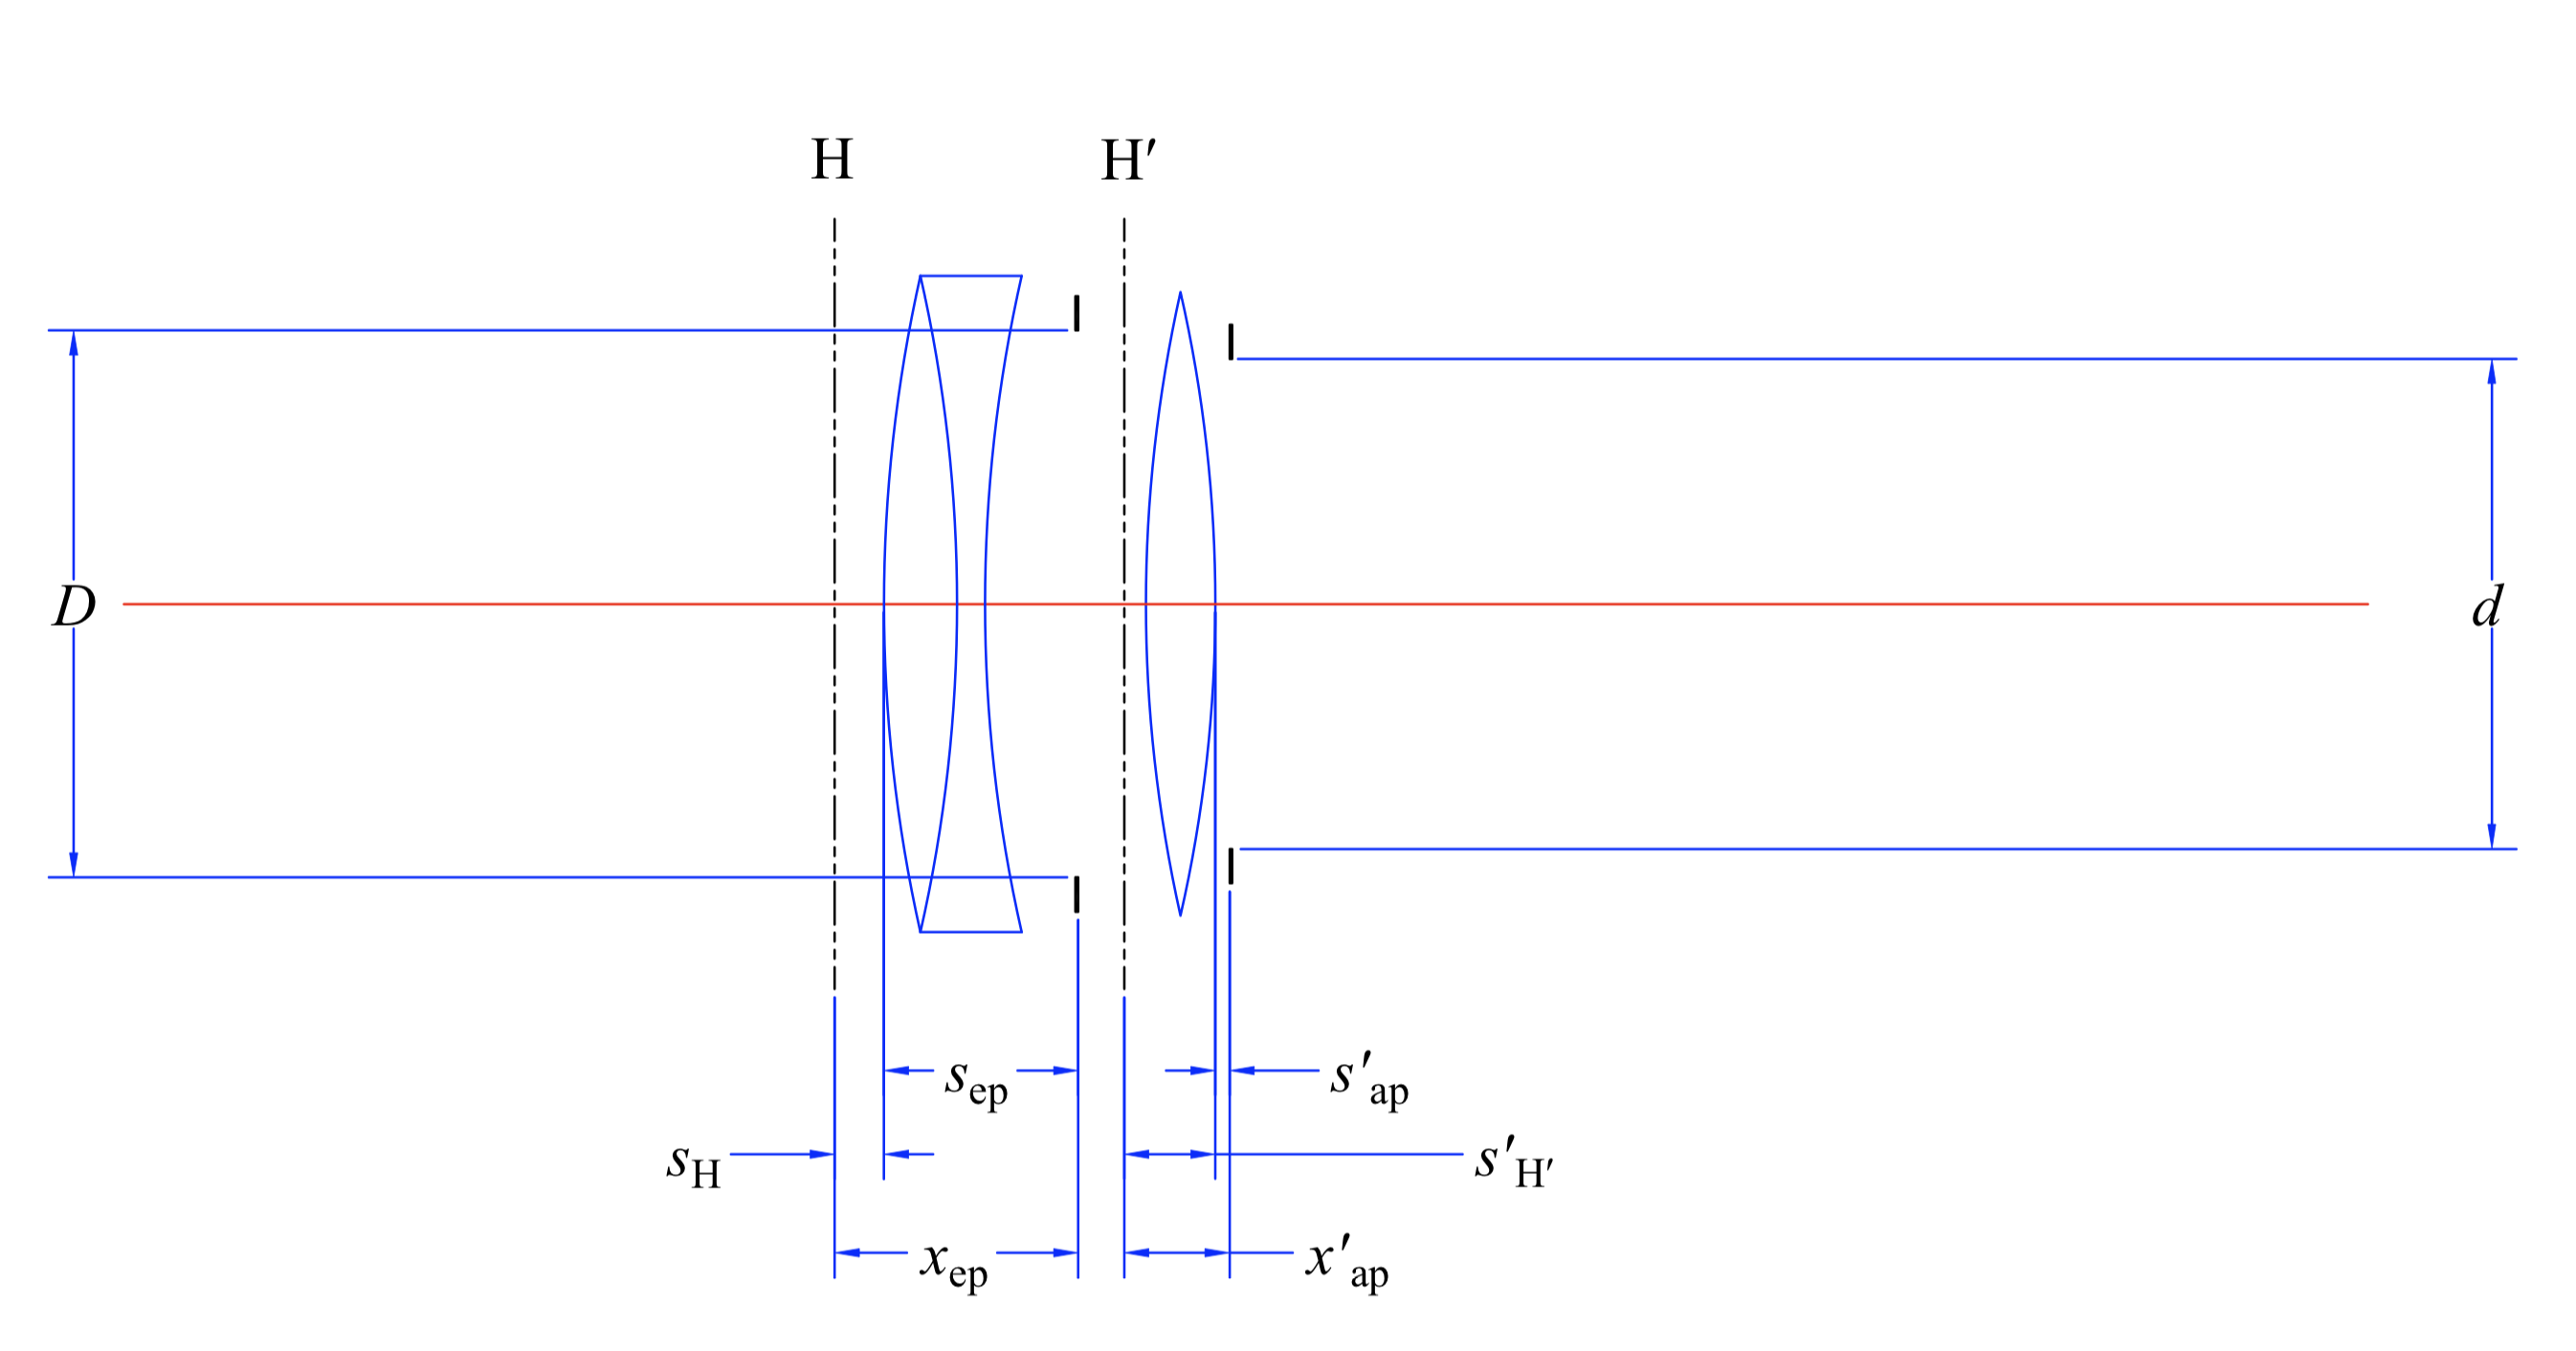
\includegraphics[width=\linewidth]{figure/fig_dofd_2} 
   \caption{Asymmetrical Lens}
   \label{fig:asymlens}
\end{figure}
%%         Figure 2. Asymmetrical Lens
The \emph{entrance pupil} is the image of the aperture stop as seen from the object side of the lens; it is the center of perspective for the lens. The \emph{exit pupil} is the image of the aperture stop as seen from the image side of the lens; it is the center of projection onto the image plane. The entrance and exit pupils may be regarded as images of each other.

Consider the lens in Figure 2 whose object and image principal planes H and H$'$ are at distances $s_\mathrm{H}$ and $s'_\mathrm{H'}$ behind the object and image vertices, and whose entrance and exit pupils are at $s_\mathrm{ep}$ and $s'_\mathrm{ap}$ behind the same vertices (by convention, left-to-right distances are positive). The entrance pupil then is at a distance $x_\mathrm{ep}$ behind H and the exit pupil is at $x'_\mathrm{ap}$ behind H$'$.
\begin{figure}[htbp] %  figure placement: here, top, bottom, or page
   \centering
   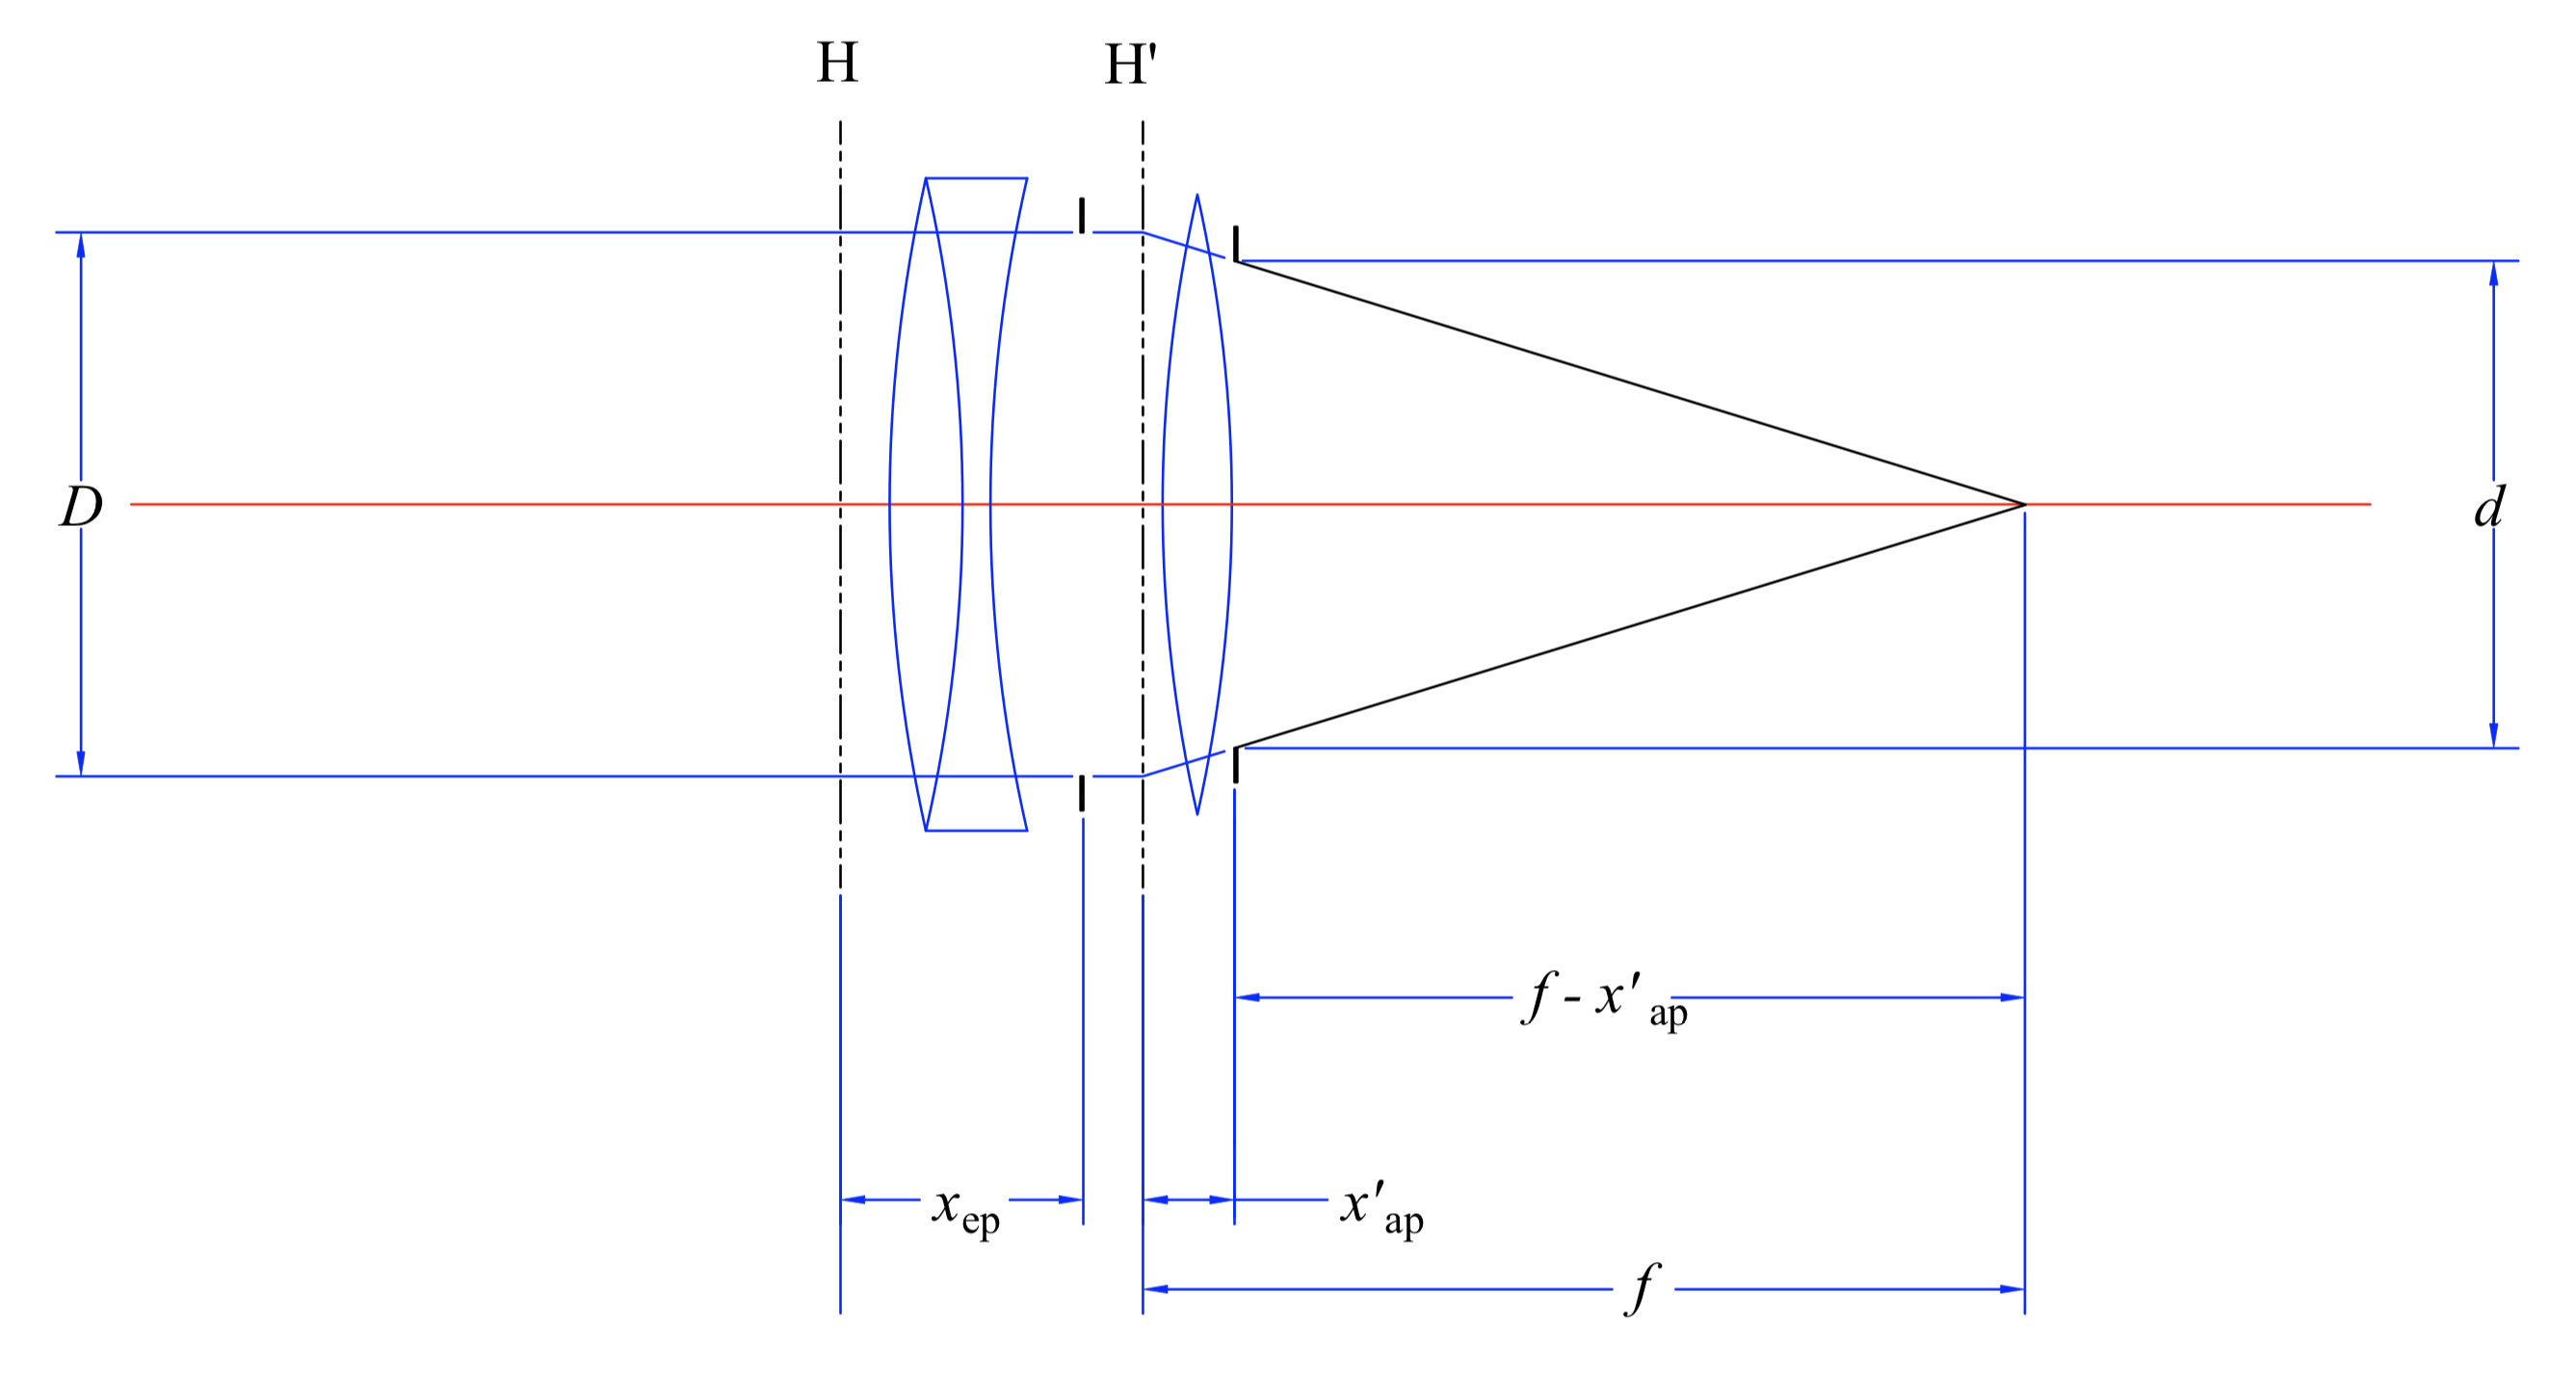
\includegraphics[width=\linewidth]{figure/fig_dofd_3} 
   \caption{Asymmetrical Lens—Entrance and Exit Pupils}
   \label{fig:asympup}
\end{figure}
%% Figure 3. Asymmetrical Lens—Entrance and Exit Pupils
%% 
%%  Page 21
The entrance and exit pupil diameters are related by the pupillary magnification
\begin{equation}
  p = \frac d D
  \label{eq:p}
  % #78
\end{equation}
%% 
In Figure~\ref{fig:asympup}, at infinity focus, the extension to H$'$ of
the cone of light from the exit pupil has diameter $D$; from similar
triangles,
\begin{equation}
  \label{eq:79}
  \frac D f = \frac d{f-x_\mathrm{ap}'}=\frac{pD}{f-x_\mathrm{ap}'}
  %  #79
\end{equation}
and
\begin{equation}
  \label{eq:80}
  x_\mathrm{ap}'=f(1-p)
  %  #80
\end{equation}

The distances $x_\mathrm{ep}$ and $x'_\mathrm{ap}$ are conjugate, so they are related by the lateral magnification $m$. In
this case, the lateral magnification is the pupillary magnification
$p$, so that
\begin{equation}
  \label{eq:xapp}
  x'_\mathrm{ap} = p x_\mathrm{ep}
\end{equation}
and
\begin{equation}
  \label{eq:xep}
  x_\mathrm{ep} = f\left(\frac1p-1\right)
  % #81
\end{equation}

\begin{figure}[htbp] %  figure placement: here, top, bottom, or page
   \centering
   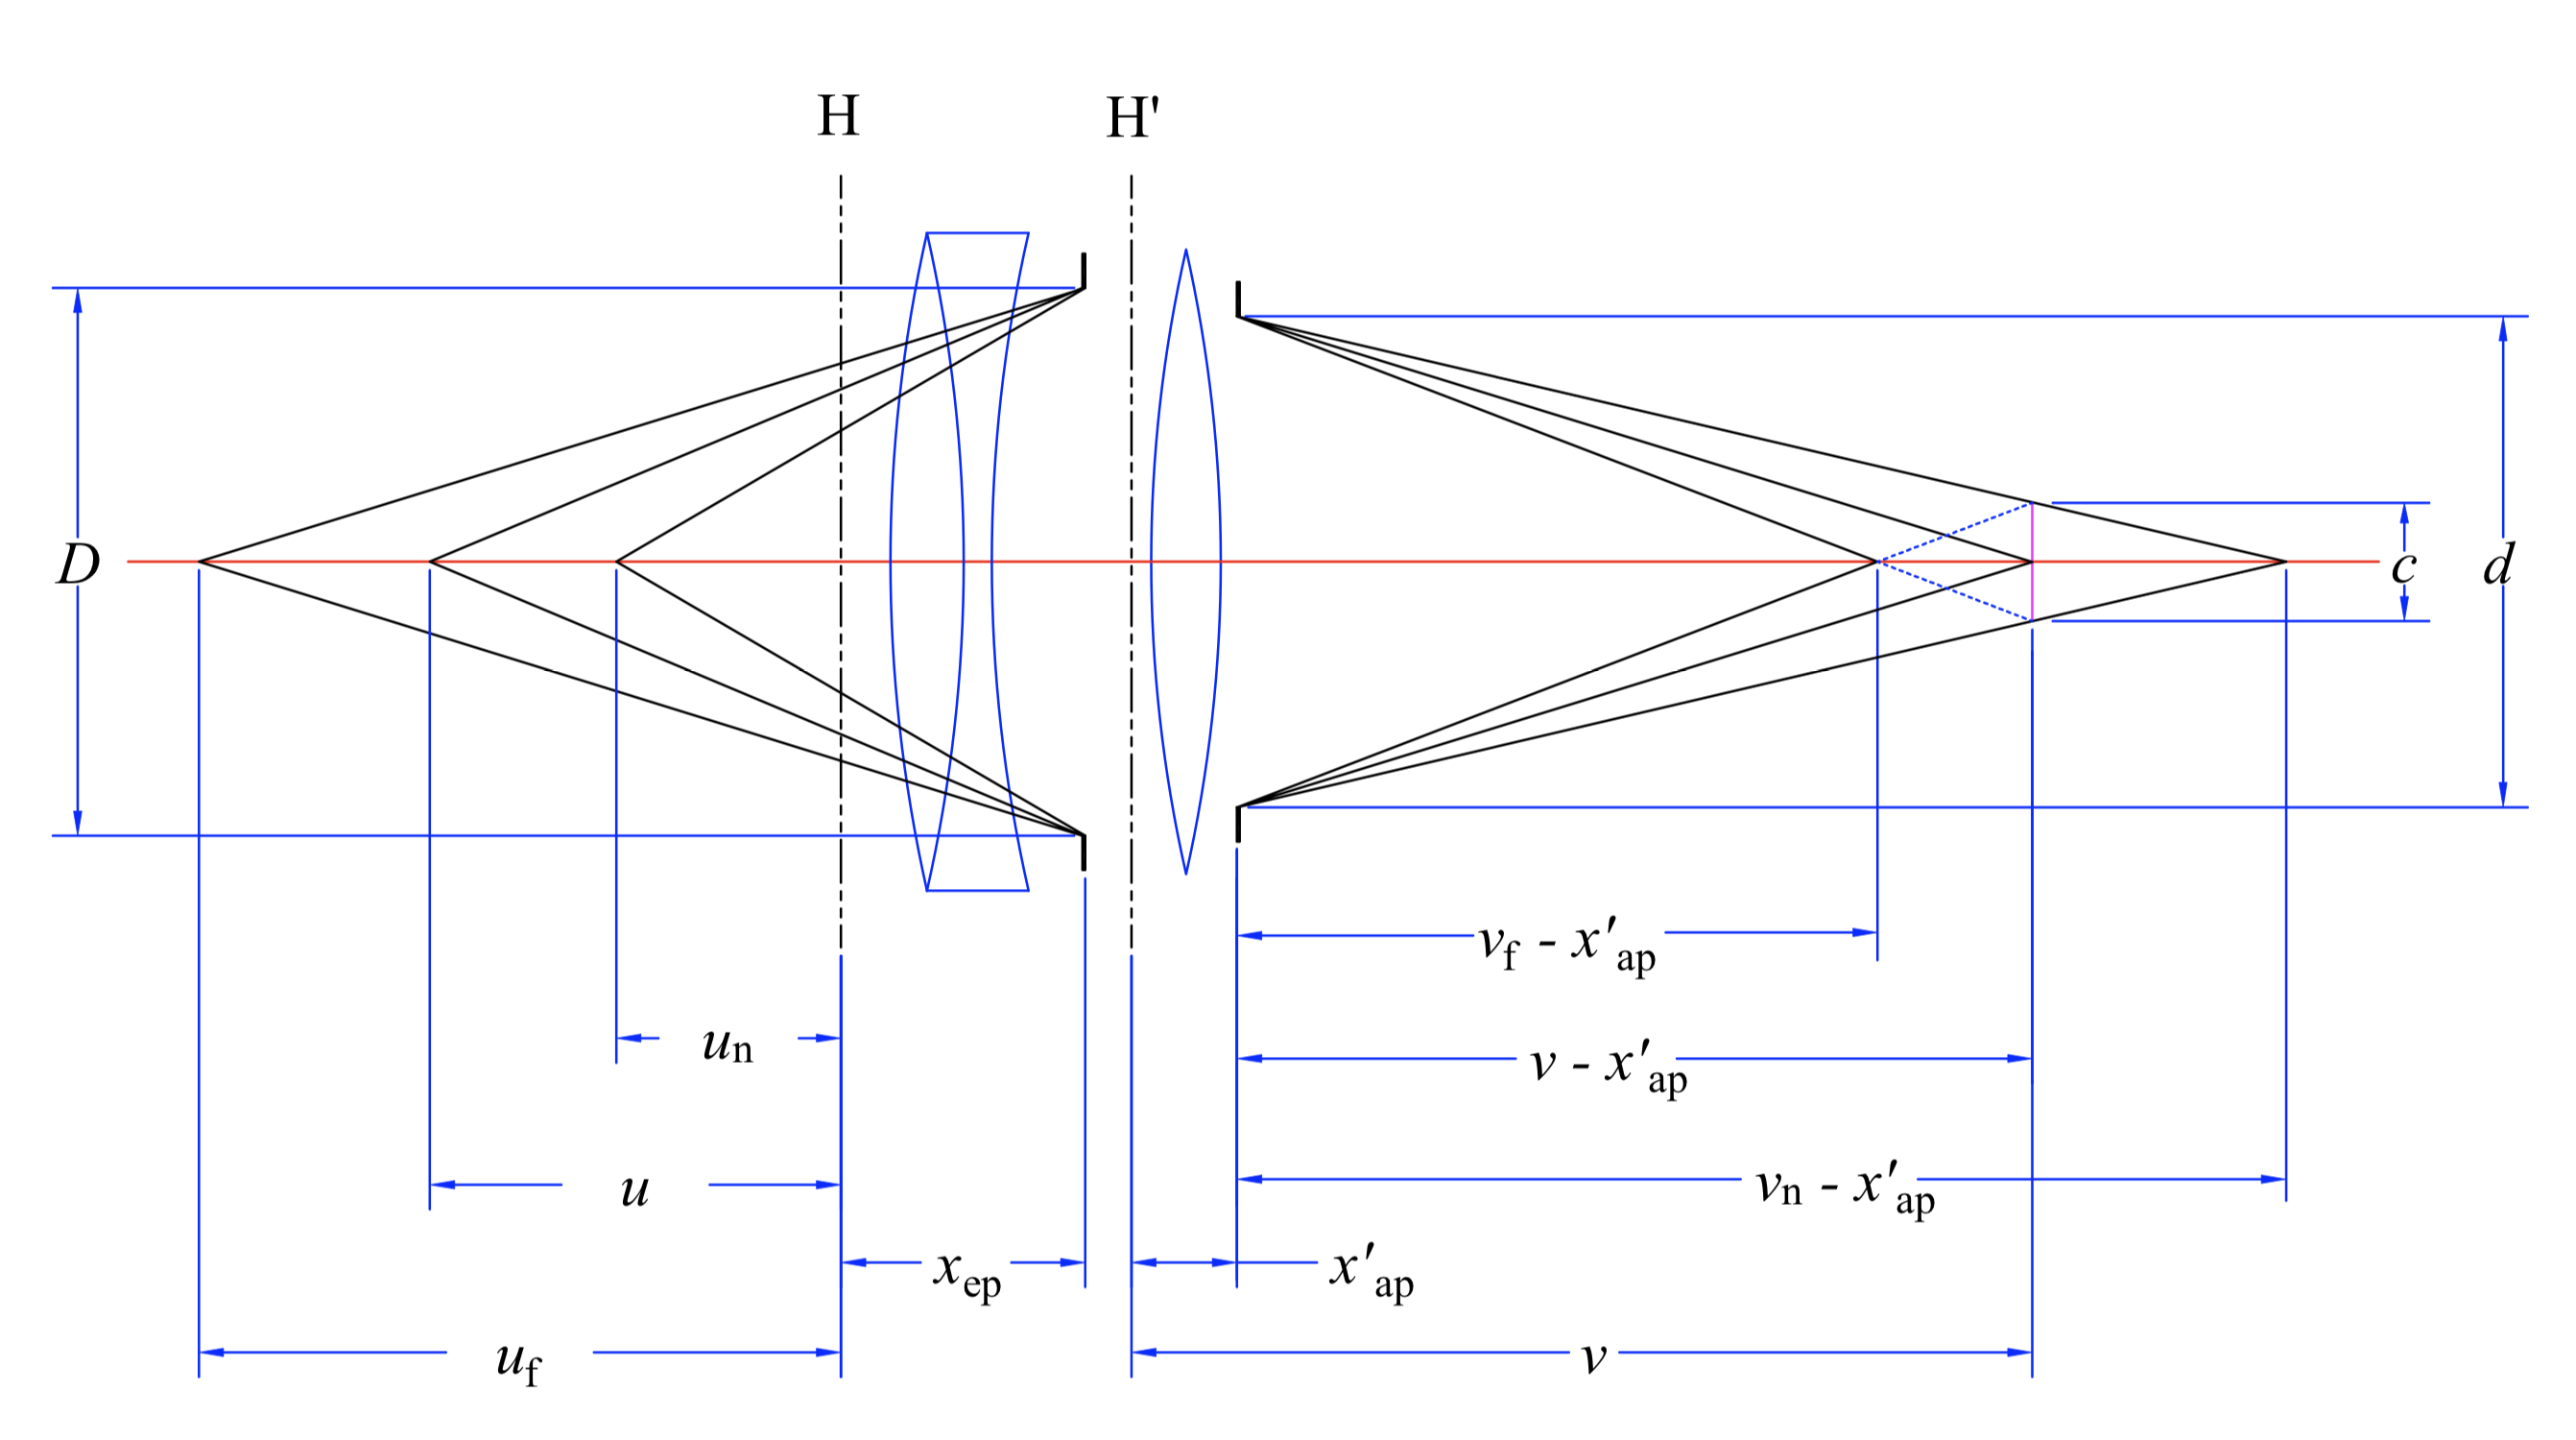
\includegraphics[width=\linewidth]{figure/fig_dofd_4} 
   \caption{DoF for Asymmetrical Lens}
   \label{fig:DOFasymlens}
\end{figure}
%% Figure 4. DoF for Asymmetrical Lens
DoF is controlled by the diameter of the lens exit pupil. In Figure 4, the near and far limits of DoF are at object distances $u_\mathrm{n}$ and $u_\mathrm{f}$, corresponding to image distances $v_\mathrm{n}$ and $v_\mathrm{f}$; at the focused image distance $v$, they form circular images of diameter $c$, the acceptable circle of confusion. From similar triangles,
\begin{equation}
\frac c d = \frac{(v_\mathrm{n}-x'_\mathrm{ap}) - (v-x'_\mathrm{ap})}{v_\mathrm{n}-x'_\mathrm{ap}} =
\frac {v_\mathrm{n} - v}{v_\mathrm{n}-x'_\mathrm{ap}} =
\frac{(v-x'_\mathrm{ap}) - (v_\mathrm{f}-x'_\mathrm{ap})}{v_\mathrm{f}-x'_\mathrm{ap}} =
\frac {v - v_\mathrm{f}}{v_\mathrm{f}-x'_\mathrm{ap}}
\label{eq:82}
\end{equation}


%% Page 22 
It usually is more convenient to work with the lens $f$-number than the exit pupil diameter;
the $f$-number is related to the lens focal length $f$ and the entrance pupil diameter $D$ by 
\begin{equation}
N = \frac f D
\end{equation}
eliminating $D$ by means of Eq. (78), the lens $f$-number then can be expressed in terms of the
exit pupil diameter as
\begin{equation}
N = \frac {pf} D
\end{equation}
Making the substitution
\begin{equation}
d = \frac {pf} N
\end{equation}
into Eq. (82) gives
\begin{equation}
   \frac {N\!c}{pf} = \frac{v_\mathrm{n} - v}{v_n - x'_\mathrm{ap}} 
                          = \frac {v - v_\mathrm{f}}{v_\mathrm{f}- x'_\mathrm{ap}}
   \label{eq:83}
   % #83
\end{equation}


\subsection{Image Space}
\label{sec:imspc}

Substituting Eq. (80) into Eq. (83) and rearranging, one arrives at several relations in image space. The image distances corresponding to the near and far limits of DoF are
\begin{equation}
   v_\mathrm{n} = \frac{fv - N\!cf\left(\frac1p - 1\right)}{f - N\!c\left(\frac1p \right)}
   \label{eq:84}
   % #84
\end{equation}
\begin{equation}
   v_\mathrm{f} = \frac{fv + N\!cf\left(\frac1p - 1\right)}{f + N\!c\left(\frac1p \right)}
   \label{eq:85}
   % #85
\end{equation}
The required focus point and $f$-number to have the DoF extend from $u_\mathrm{n}$ to $u_\mathrm{f}$ are
\begin{equation}
   v = \frac{2v_\mathrm{n}v_\mathrm{f} - (v_\mathrm{n} +v_\mathrm{f})f(1-p)}{v_\mathrm{n} +v_\mathrm{f}-2f(1-p)}
   \label{eq:86}
   % #86
\end{equation}
\begin{equation}
   N = \frac{pf}c \frac{v_\mathrm{n} - v_\mathrm{f}}{v_\mathrm{n} +v_\mathrm{f}-2f(1-p)}
   \label{eq:87}
   % #87
\end{equation}
If $v_\mathrm{n}$ or $v_\mathrm{f}$ in Eq. (83) is replaced by an arbitrary distance $v_\mathrm{d}$, corresponding to a defocused
point object at object distance $u_\mathrm{d}$, the diameter of the resulting blur spot is given by
\begin{equation}
   k = \frac{pf}N \frac{|v_\mathrm{d} - v|}{v_\mathrm{d} + f(p-1)}
   \label{eq:88}
   % #88
\end{equation}

\subsection{Object Space}
\label{sec:objspc}

Rearranging Eq. (5) to
\begin{equation}
  \label{eq:5v}
  v = \frac{uf}{u-f}\quad,
\end{equation}
%
%% Page 23
substituting into Eqs. (84) through (88), and again rearranging, one
arrives at the corresponding relations in object space. The near and
far limits of DoF are
\begin{eqnarray}
     u_\mathrm{n} & = & \frac{uf^2 -  N\!cf\left(\frac1p-1\right)(u-f)}{f^2 + N\!c(u-f)}\label{eq:89}\\
     u_\mathrm{f} & = & \frac{uf^2 + N\!cf\left(\frac1p-1\right)(u-f)}{f^2 - N\!c(u-f)}\label{eq:90}
\end{eqnarray}
When $u_\mathrm{f} = \infty$, the focus distance is the hyperfocal distance
$u_\mathrm{h}$, where
\begin{equation}
  \label{eq:uh2}
  u_\mathrm{h} = \frac{f^2}{N\!c} + f
\end{equation}
the same as for a symmetrical lens. Solving for the near limit of DoF gives
\begin{equation}
  \label{eq:3un}
  u_\mathrm{n} = \frac12 \left(\frac{f^2}{N\!c} + f - f\left(\frac1p-1\right)\right)\quad,
  % #92
\end{equation}
or slightly less than half the hyperfocal distance.

The required focus distance and $f$-number to have the DoF extend from
$u_\mathrm{n}$ to $u_\mathrm{f}$ are
\begin{equation}
  \label{eq:93}
  u = \frac{2u_\mathrm{n}u_\mathrm{f} +
    (u_\mathrm{n}+u_\mathrm{f})f\left(\frac1p-1\right)}{u_\mathrm{n}+u_\mathrm{f}+2f\left(\frac1p-1\right)}
  % #93
\end{equation}
and
\begin{equation}
  \label{eq:94}
  N=\frac{f^2}c\frac{u_\mathrm{f}-u_\mathrm{n}}{(u_\mathrm{n}-f)\left[u_\mathrm{f}+f\left(\frac1p-1\right)\right]+(u_\mathrm{f}-f)\left[u_\mathrm{n}+f\left(\frac1p-1\right)\right]}
  % #94
\end{equation}
For a defocused point object at object distance $u_\mathrm{d}$, the diameter of
the blur spot is
\begin{equation}
  \label{eq:95}
  k  = \frac{pfm}N\frac{|u_\mathrm{d}-u|}{u_\mathrm{d}+(u_\mathrm{d}-f)(p-1)}
  % #95
\end{equation}
%% k & pfm ud −u
%% N ud+(ud−f)(p−1)
From Eqs. (44)\footnote{Eq. (44) is inapplicable to an asymmetrical lens, so Eq. (96) as
shown here is incorrect. See the Erratum at the end
of this document for the correct value.} and (95), the “relative blur”
is
\begin{equation}
  \label{eq:96}
  k_r=\frac k {m_\mathrm{d}} = \frac m{m+1} \frac p N
  \frac{u_\mathrm{d}|u_\mathrm{d}-u|}{u_\mathrm{d}+(u_\mathrm{d}-f)(p-1)}
  % #96
\end{equation}
For $u_\mathrm{d} \gg f$,
\begin{equation}
  \label{eq:97}
  k_r\approx \frac m{m+1} \frac{|x_\mathrm{d}|}N\quad,
  % #97
\end{equation}
the same as Eq. (45) for a symmetrical lens.


The DoF in front of the focused object is
\begin{equation}
  \label{eq:98}
  u-u_\mathrm{n}=\frac{\left[N\!cf\left(\frac 1p-1\right) + N\!cu\right](u-f)}{f^2
    + N\!c(u-f)}
  % #98
\end{equation}
%% Page 24 
The DoF beyond the focused object is
\begin{equation}
u_\mathrm{f}-u=\frac{\left[N\!cf\left(\frac 1 p -1\right) + N\!cu\right](u-f)}{f^2-N\!c(u-f)}
   %% #(99)
   \label{eq:dofbfo}
\end{equation}
The front and rear DoF can be expressed in terms of the magnification by making the substitution
\begin{equation}
u-f = \frac f m
\end{equation}
 into the equations for front and rear DoF and rearranging:
\begin{equation}
u-u_\mathrm{n} = \frac{NC\left(1+ \frac m p\right)}{m^2\left(1+\frac{NC}{fm}\right)}
\end{equation}
and
\begin{equation}
u_\mathrm{f}-u = \frac{NC\left(1+ \frac m p\right)}{m^2\left(1-\frac{NC}{fm}\right)}
\end{equation}
The front:rear DoF ratio is 
\begin{equation}
   \frac{u - u_\mathrm{n}}{u_\mathrm{f}-u} =  \frac{f^2 - NC(u-f)}{f^2 + NC(u-f)} = \frac{fm - NC}{fm + NC}
   % #102
   \label{eq:frdofratio}
\end{equation}
the same as for a symmetrical lens.

The total DoF is
\begin{equation}
   u_\mathrm{f} - u_\mathrm{n} = \frac{2N\!cf^2\left[u+f\left(\frac 1 p -1 \right)\right](u-f)}{f^4-N^2c^2(u-f)^2}
   % #103
   \label{eq:totdof}
\end{equation}
or, in terms of the magnification,
\begin{equation}
   u_\mathrm{f} - u_\mathrm{n} = \frac{2f\left(\frac 1 m + \frac 1 p\right)}{\frac{fm}{N\!c}-\frac{N\!c}{fm}}
   % #104
   \label{eq:magdof}
\end{equation}
At the hyperfocal distance, the two terms in the denominator are equal, and the DoF is
 infinite. When $u\ll u_\mathrm{h}$, the second term in the denominator is small, and
\begin{equation}
   u_\mathrm{f} - u_\mathrm{n} = \frac{2N\!c}{m}\left(\frac 1 m + \frac 1 p\right)
   % #105
   \label{eq:DOFapprox}
\end{equation}

%% Page 25

\subsection{Effect of Lens Asymmetry}

The effect of asymmetry is greatest when a lens for which $p$ differs substantially from unity is used at high magnification. Accordingly, large-format photographers usually can neglect the pupillary magnification: most medium- and short-focus large-format lenses have $p$ close to 1, and telephoto large-format lenses seldom are used at high magnification; for example, at $m = 0.1$, a telephoto lens with $p  = 0.75$ has 3\% greater DoF than a lens with $p = 1$. This is fortunate, because the asymmetrical-lens DoF formulae are sufficiently complex that their use in the field is impractical without a programmable calculator or handheld computer; moreover, the image-side formulae for setting focus and $f$-number require absolute image distances, which can be difficult to measure.

The effect of asymmetry can be significant for telephoto macro lenses for hand cameras: at $m = 1$, a lens with $p = 0.4$ has 75\% greater DoF than a lens with $p = 1$. Again, the application of the asymmetrical-lens DoF formulae to practical situations can be difficult, albeit for different reasons than with large-format lenses. Distance scales on hand-camera lenses usually indicate object-to-image distance rather than object distance, and the difference is significant at close distances. Conversion between the two distances is not always simple, because many close-focusing hand-camera lenses use internal focusing, so that pupillary magnification as well as focal length change with focus distance. Lens manufacturers have this information readily available; consequently, lens DoF scales or charts provided by the lens manufacturer usually provide the most accurate estimates of DoF. In any event, it is obvious from Eq. (105) that Eq. (25) should not be used to estimate closeup DoF for highly asymmetrical lenses.

\subsection{Symmetrical Lens}

In the case of a symmetrical lens for which $p = 1$, the relations in image and in object space reduce to the simpler ones given at the beginning of this paper and in most other treatments of depth of field. Except for closeup work with substantially asymmetrical lenses, the error resulting from use of the symmetrical-lens formulae usually is minimal.

\section{Diffraction}
\label{sec:diffraction}


Even with a perfect (i.\,e., aberration-free) lens, a point object in
focus is not imaged as a point, but rather as a disk surrounded by
dark and light rings; the pattern is known as the Airy\footnote{After
  British astronomer Sir George Airy (1801–-1892), who, in 1835, was
  the first to describe the pattern mathematically.} pattern. The
phenomenon responsible for the Airy pattern is diffraction, the
bending of light as it passes an edge. Diffraction is a consequence of
the wave nature of light, and is a fundamental physical constraint for
lenses of all designs. The diameter of the pattern to the first dark
ring is known as the Airy disk, and is given by
\begin{equation}
  \label{eq:airy}
   k_\mathrm{Airy} = 2.44\lambda N(1+m)\quad,
\end{equation}
%% kAiry &2.44λN(1+m),
where $\lambda$ is the wavelength of the light, $N$ is the lens
$f$-number, and $m$ the magnification. Two image points are resolved
when their separation is sufficient for them to be recognized as
arising from two distinct objects; the resolution is the distance by
which the two objects must be separated. According the empirical (but
widely used) Rayleigh\footnote{After John William Strutt, third Baron
  Rayleigh (1842–1919), Nobel laureate in physics, 1904.} criterion,
two Airy disks can be resolved when separated by one radius; other
resolution criteria, such as the Dawes\footnote{After British
  astronomer William Rutter Dawes (1799–1868).} and Sparrow, specify
slightly different separations. Closely related to resolution, and
perhaps more commonly used, is resolving power, given by
\begin{equation}
  \label{eq:respow}
  \mathrm{RP} = \frac 1 R
  %% RP = 1 R
\end{equation}
Resolving power corresponds to a spatial frequency whose period is the width of a pair of lines, one dark and one light. When describing photographihc optics, resolving power usually is specified in line pairs per millimeter, or lp/mm.

Visible light comprises a mixture of wavelengths that range from
approximately 400\,nm to 700\,nm; the most conservative approach would
be to assume a wavelength of 700\,nm, but common practice is to assume
a yellow-green wavelength; choosing 546\,nm,
\begin{equation}
  \label{eq:airy2}
  k_\mathrm{Airy}  = 0.00133N(1+m)\,[\mathrm{mm}]\quad,
  %% kAiry = 0.00133N(1+m)mm, (106)
\end{equation}
or approximately
\begin{equation}
  \label{eq:airy3}
   k_\mathrm{Airy}  =\frac{N(1+m)}{750}\,[\mathrm{mm}]\quad,
   %% kAiry = N (1+ m) mm (107) 750
\end{equation}
Diffraction by the aperture stop places an absolute limit on the resolution of even a perfect lens. After the Rayleigh criterion, the diffraction-limited resolution derives from the radius of the Airy disk: at 546\,nm,
\begin{equation}
  \label{eq:Rdiff}
  R_\mathrm{diff} = \frac{N (1+ m)}{1500}\,[\mathrm{mm}]\quad ,
  %% Rdiff & N (1+ m) mm , 1500
\end{equation}
or in terms of resolving power,
\begin{equation}
  \label{eq:RP}
  \mathrm{RP} = \frac{1500}{N(1+m)}\,[\mathrm{lp/mm}]\quad,
\end{equation}
which leads the commonly cited
\begin{equation}
  \label{eq:RPmax}
  \mathrm{RP_\mathrm{max}}  = \frac{1500}N\,[\mathrm{lp/mm}]
\end{equation}
at infinity focus. For a given resolution, there is a maximum $f$-number. If it is required that the resolution not exceed the CoC, then $R_\mathrm{diff} = c$, and from Eq. \ref{eq:Rdiff},
\begin{equation}
   \label{eq:Nmax}
   N_\mathrm{max}=\frac{1500c}{(1+m)\,[\mathrm{mm}]}
\end{equation}
For example, if 0.025\,mm were the acceptable circle of confusion for a 35\,mm image, the maximum usable $f$-number at infinity focus ($m = 0$) would be 37.5; at $m = 1$, the maximum $f$-number would be 18.75. The effects of diffraction obviously become more important in closeup photography.

Recall from Eq. (76) that for a given DoF, when perspective and
image framing are held constant by suitable lens selection, the
required $f$-number is proportional to the camera format. From
Eq. (109), the diffraction-limited resolving power is inversely
proportional to the $f$-number, so that the blur spot is inversely proportional to the camera format. Because the required enlargement also is inversely proportional to the camera format, the diffraction- limited resolution is largely independent of camera format. This is less true when no DoF is required and only the plane of focus is of interest, so that the lens can be used at its optimum $f$-number. Most large-format lenses are sharpest between approximately \f{16} and \f{22}, while most 35\,mm lenses are best at between \f8 and \f{11}. Consequently, although a 4$\times$5 image has half the diffraction-limited resolution of a 35\,mm image, it requires only 1⁄4 the enlargement. Of course, both cases consider only the optically determined resolving power and not the structure of the imaging medium. Considerable image degradation results from enlargement of small-format images, giving the larger formats an advantage.

\subsection{Combined Defocus and Diffraction}
\label{sec:comb-defoc-diffr}


The effects of defocus and diffraction combine at all
$f$-numbers. There is no simple numerical expression for the
combination; however, common empirical rules for combination of
resolutions of different components of optical systems have been
\begin{equation}
  \label{eq:110}
  R_\mathrm{T}=r_1 + R_2 + \ldots + R_n
  % #110
\end{equation}
or sometimes
\begin{equation}
  \label{eq:111}
  R^x_\mathrm{T}=R^x_1 + R^x_2 + \ldots + R^x_n
  % #111
\end{equation}
with $x$ usually close to 2. There is little precedent for using these formulae to combine different aspects of the same component, but Hansma (1996) suggested a root-square combination of defocus and diffraction blur spots. The size of the composite blur spot then would be given by
\begin{equation}
  \label{eq:112}
  c_\mathrm{T}=\sqrt{k^2_\mathrm{def}+k^2_\mathrm{diff}}
  % #112
\end{equation}
or
\begin{equation}
  \label{eq:113}
  c_\mathrm{T} = \sqrt{ \left[ \frac\Dv{2N(1+m)}\right]^2 + \left[\frac N{K_\lambda}(1+m)\right]^2}
  % #113
\end{equation}
where \Dv\ is the focus spread $v_\mathrm{n} - v_\mathrm{f}$ and $K_\lambda$ is a constant related to the effective size of the diffraction blur spot.

\subsection{Optimum $f$-Number}
\label{sec:optimum-f-number}

At any given focus spread, as $f$-number is increased, the size of the defocus blur spot decreases while the size of the diffraction blur spot increases, suggesting that there may be an optimum $f$-number that minimizes the combined effect of defocus and diffraction, resulting in the sharpest possible image. Hansma determined such a minimum by differentiating Eq. (113) with respect to $N$ and setting the result equal to zero; the result is
\begin{equation}
  \label{eq:114}
  N_\mathrm{min} = \frac1{1+m}\sqrt{\frac{K_\lambda}2 \Dv}
  % #114
\end{equation}
Substitution of Eq. (114) into Eq. (113) and rearranging shows that
\begin{equation}
  \label{eq:114+}
  k_\mathrm{def} = k_\mathrm{diff} = \sqrt{\frac \Dv{2K_λ}}
\end{equation}
so that the total blur spot is minimized when the contributions of defocus and diffraction are equal. A combination of defocus and diffraction using Eq. (111) with any value of $x$ leads to the same result as Eq. (114).

Hansma used $K_λ = 750\,\mathrm{mm}^{-1}$, corresponding to the diameter of the Airy disk at
$λ = 546\,\mathrm{nm}$, for the size of the diffraction blur spot; however, he based resolving power on the radius of the combined blur spot, using
\begin{equation}
\mathrm{RP}= \frac2 {c_\mathrm{T}}
\end{equation}
The resulting resolving power vs.\ $f$-number at various focus spreads is shown in Figure 5. The curve labeled ‘\textsf{\small Diffr}’ shows resolving power at the diffraction limit, corresponding to the plane of focus. All curves assume infinity focus so that $m = 0$.
\begin{figure}[htbp] %  figure placement: here, top, bottom, or page
   \centering
   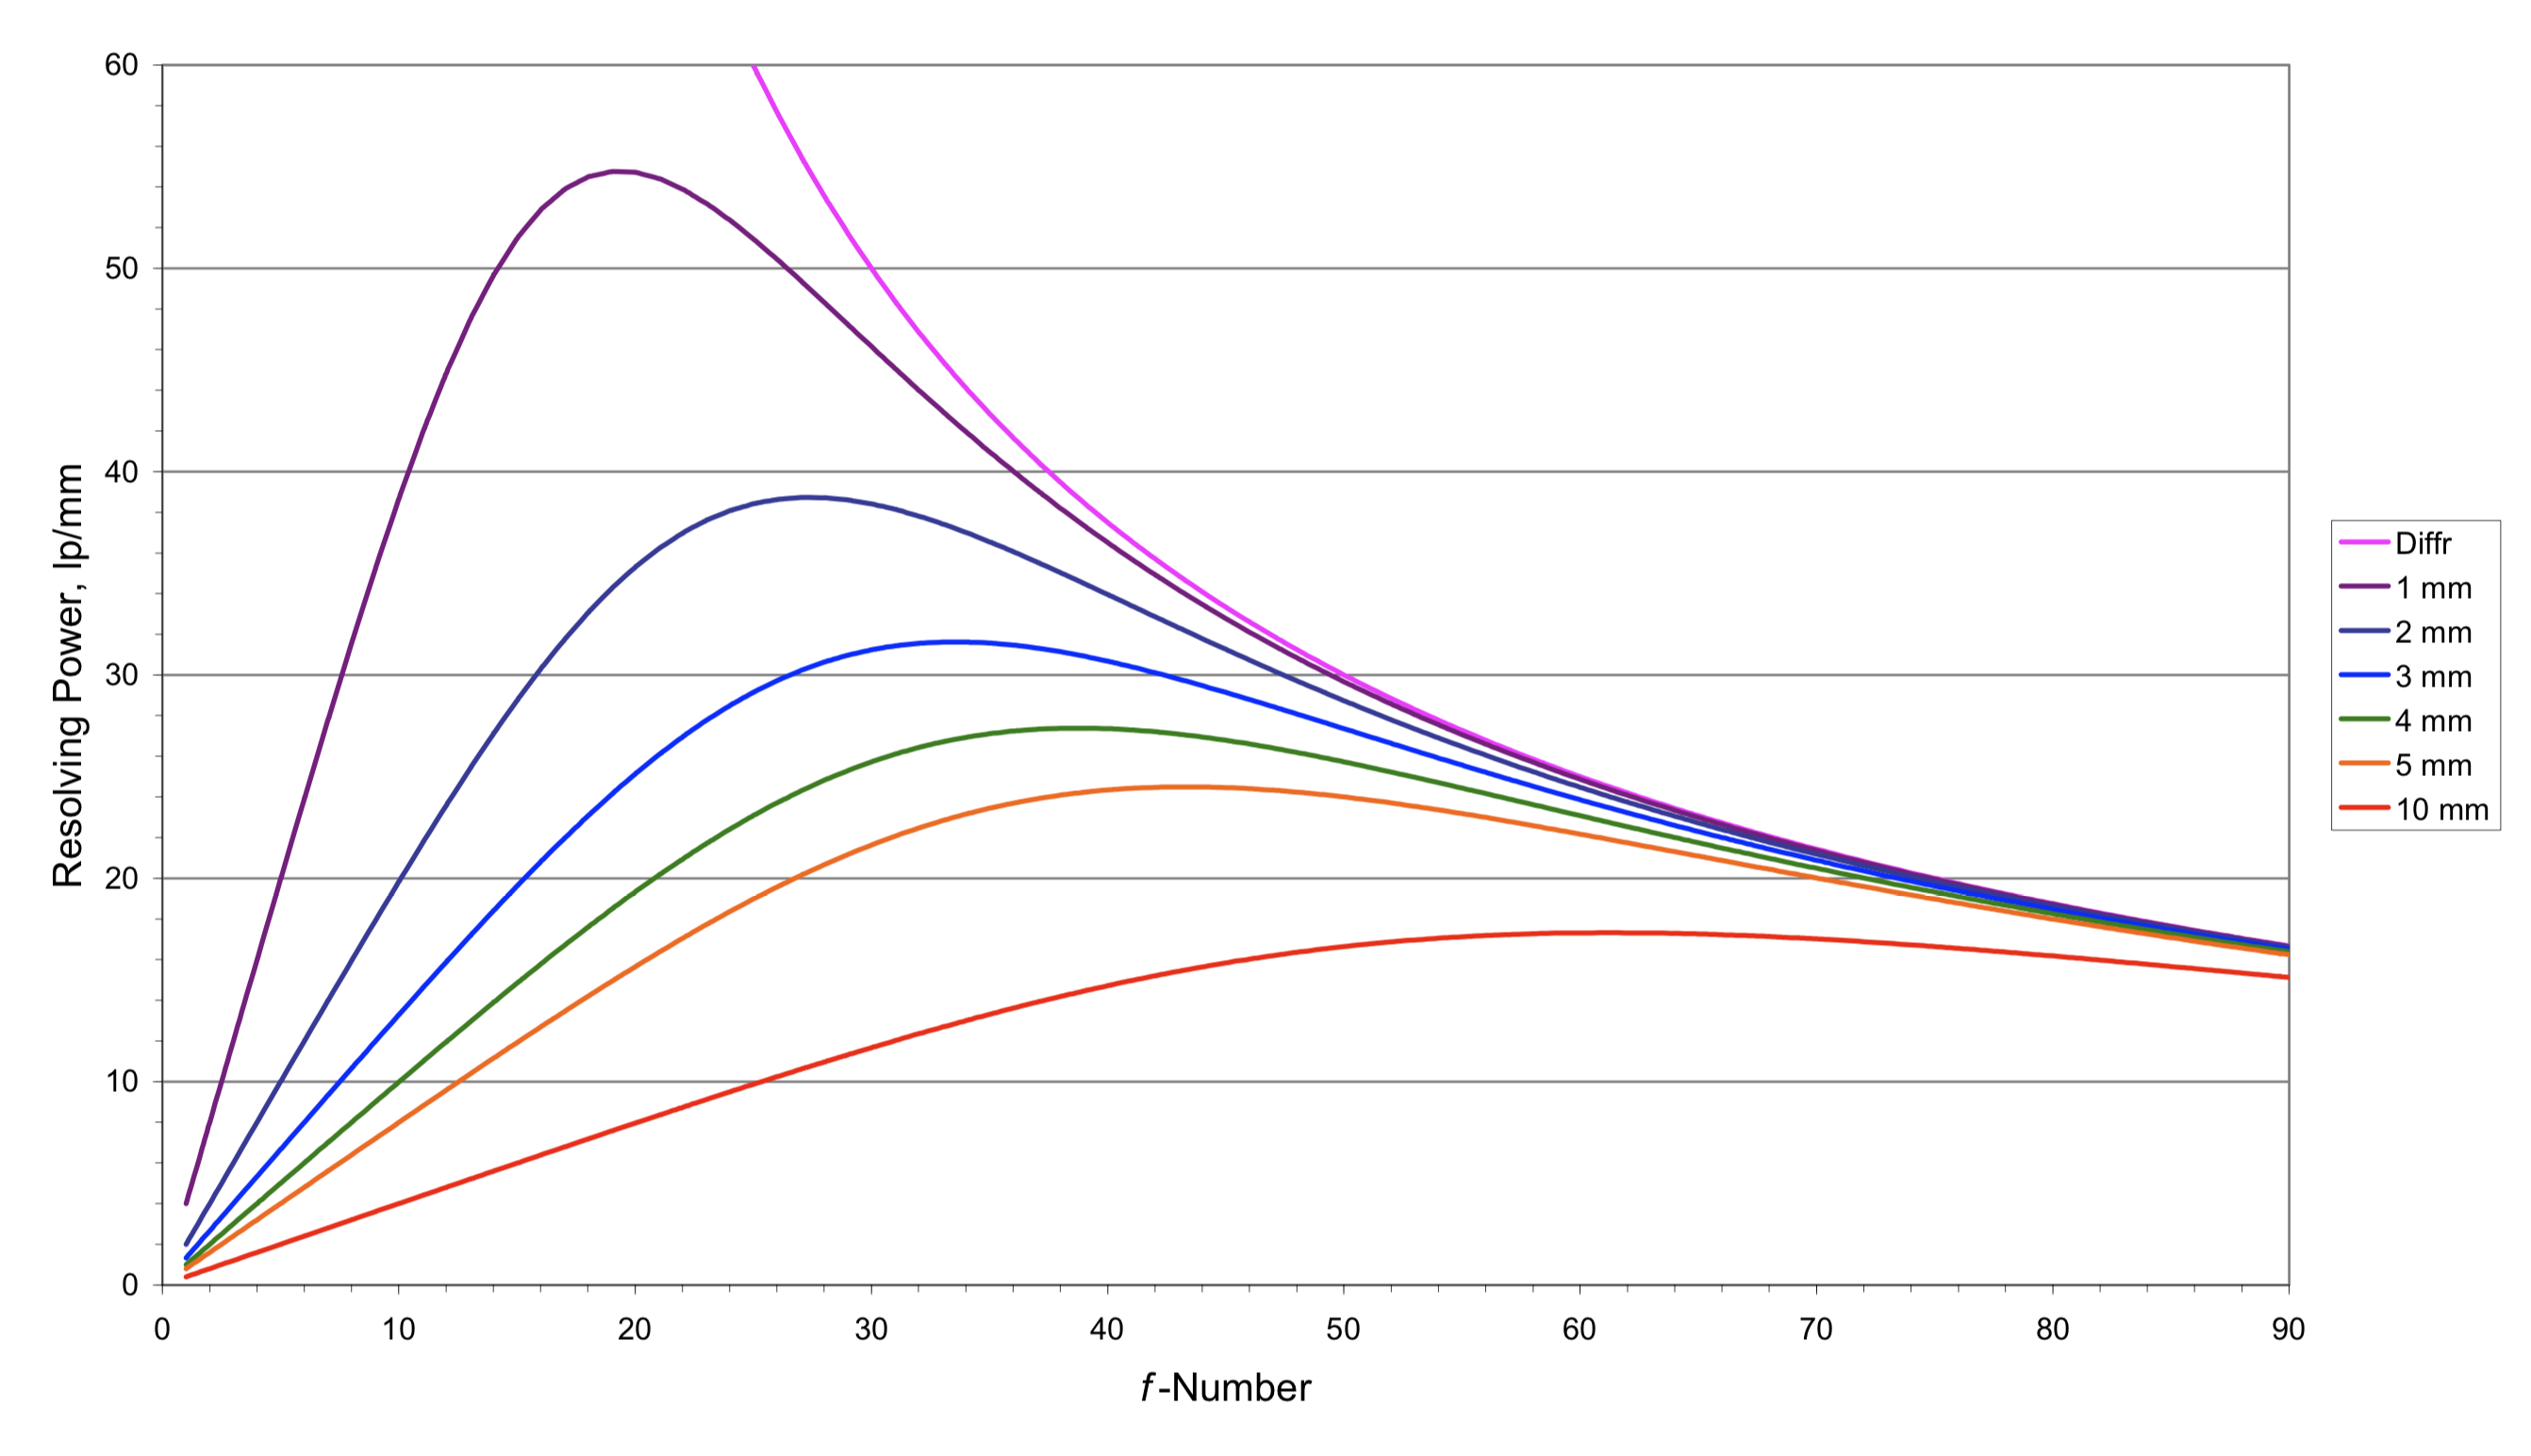
\includegraphics[width=\linewidth]{figure/fig_dofd_5} 
   \caption{Resolving Power vs.\ $f$-Number at Various Focus Spreads---Hansma}
   \label{fig:respow}
\end{figure}
%% Figure 5. Resolving Power vs. $f$-Number at Various Focus Spreads—Hansma
The results suggest considerable loss of sharpness when the $f$-number is determined by the conventional method, especially at small focus spreads. The maximum resolving power decreases rapidly with focus spread; considerable improvement results from anything, such as camera movements, that can decrease the focus spread.
\subsection{Modulation Transfer Function}

Using a single number to indicate sharpness is convenient but provides an incomplete description of image quality. Although it may give information about the finest detail that can be recognized, it gives no information about image contrast, which is as important as resolution in the perception of sharpness. Image detail does not simply vanish at a point where the separation of elements is sufficiently small, but rather, contrast decreases steadily as detail becomes finer, and eventually the contrast reaches zero. The modulation transfer function (MTF) describes the ability of an optical system to transfer contrast from the object to the image. The most convenient target is a linear array whose luminance varies sinusoidally with spatial frequency, commonly given as lp/mm, but perhaps more properly as cycles/mm. The spatial frequency of the target usually varies from very low to a value that is beyond what the optical system can transfer.

The contrast is given by
\begin{equation}
C = \frac{L_\mathrm{max} - L_\mathrm{min}}{L_\mathrm{max} + L_\mathrm{min}}
\end{equation}
where $L_\mathrm{max}$ and $ L_\mathrm{min}$ are the maximum and minimum luminances of the object or image. Because of the similarity to amplitude modulation in communications, the contrast commonly is referred to as modulation. Modulation transfer is
\begin{equation}
\mathrm{MTF} = \frac{M_\mathrm i}{M_\mathrm o}\quad,
\end{equation}
where $M_\mathrm i$ is the modulation of the image and $M_\mathrm o$ is the modulation of the target. The modulation transfer function gives the modulation transfer as a function of defocus, $f$-number, and spatial frequency. In the discussion that follows, a sinusoidal target is assumed in all cases.

For a diffraction-limited lens with no defocus, 
MTF is 
\begin{equation}
   \mathrm{MTF}(N,v) = \frac2\pi(\phi - \cos\phi\sin\phi)
   % # 115
   \label{eq:MTF2}
\end{equation}
where
\begin{equation}
\phi = \cos^{-1}\lambda vN(1+m)
\end{equation}
The MTFs for a diffraction-limited lens at various $f$-numbers are shown in Figure~\ref{fig:MTF}.
\begin{figure}[htbp] %  figure placement: here, top, bottom, or page
   \centering
   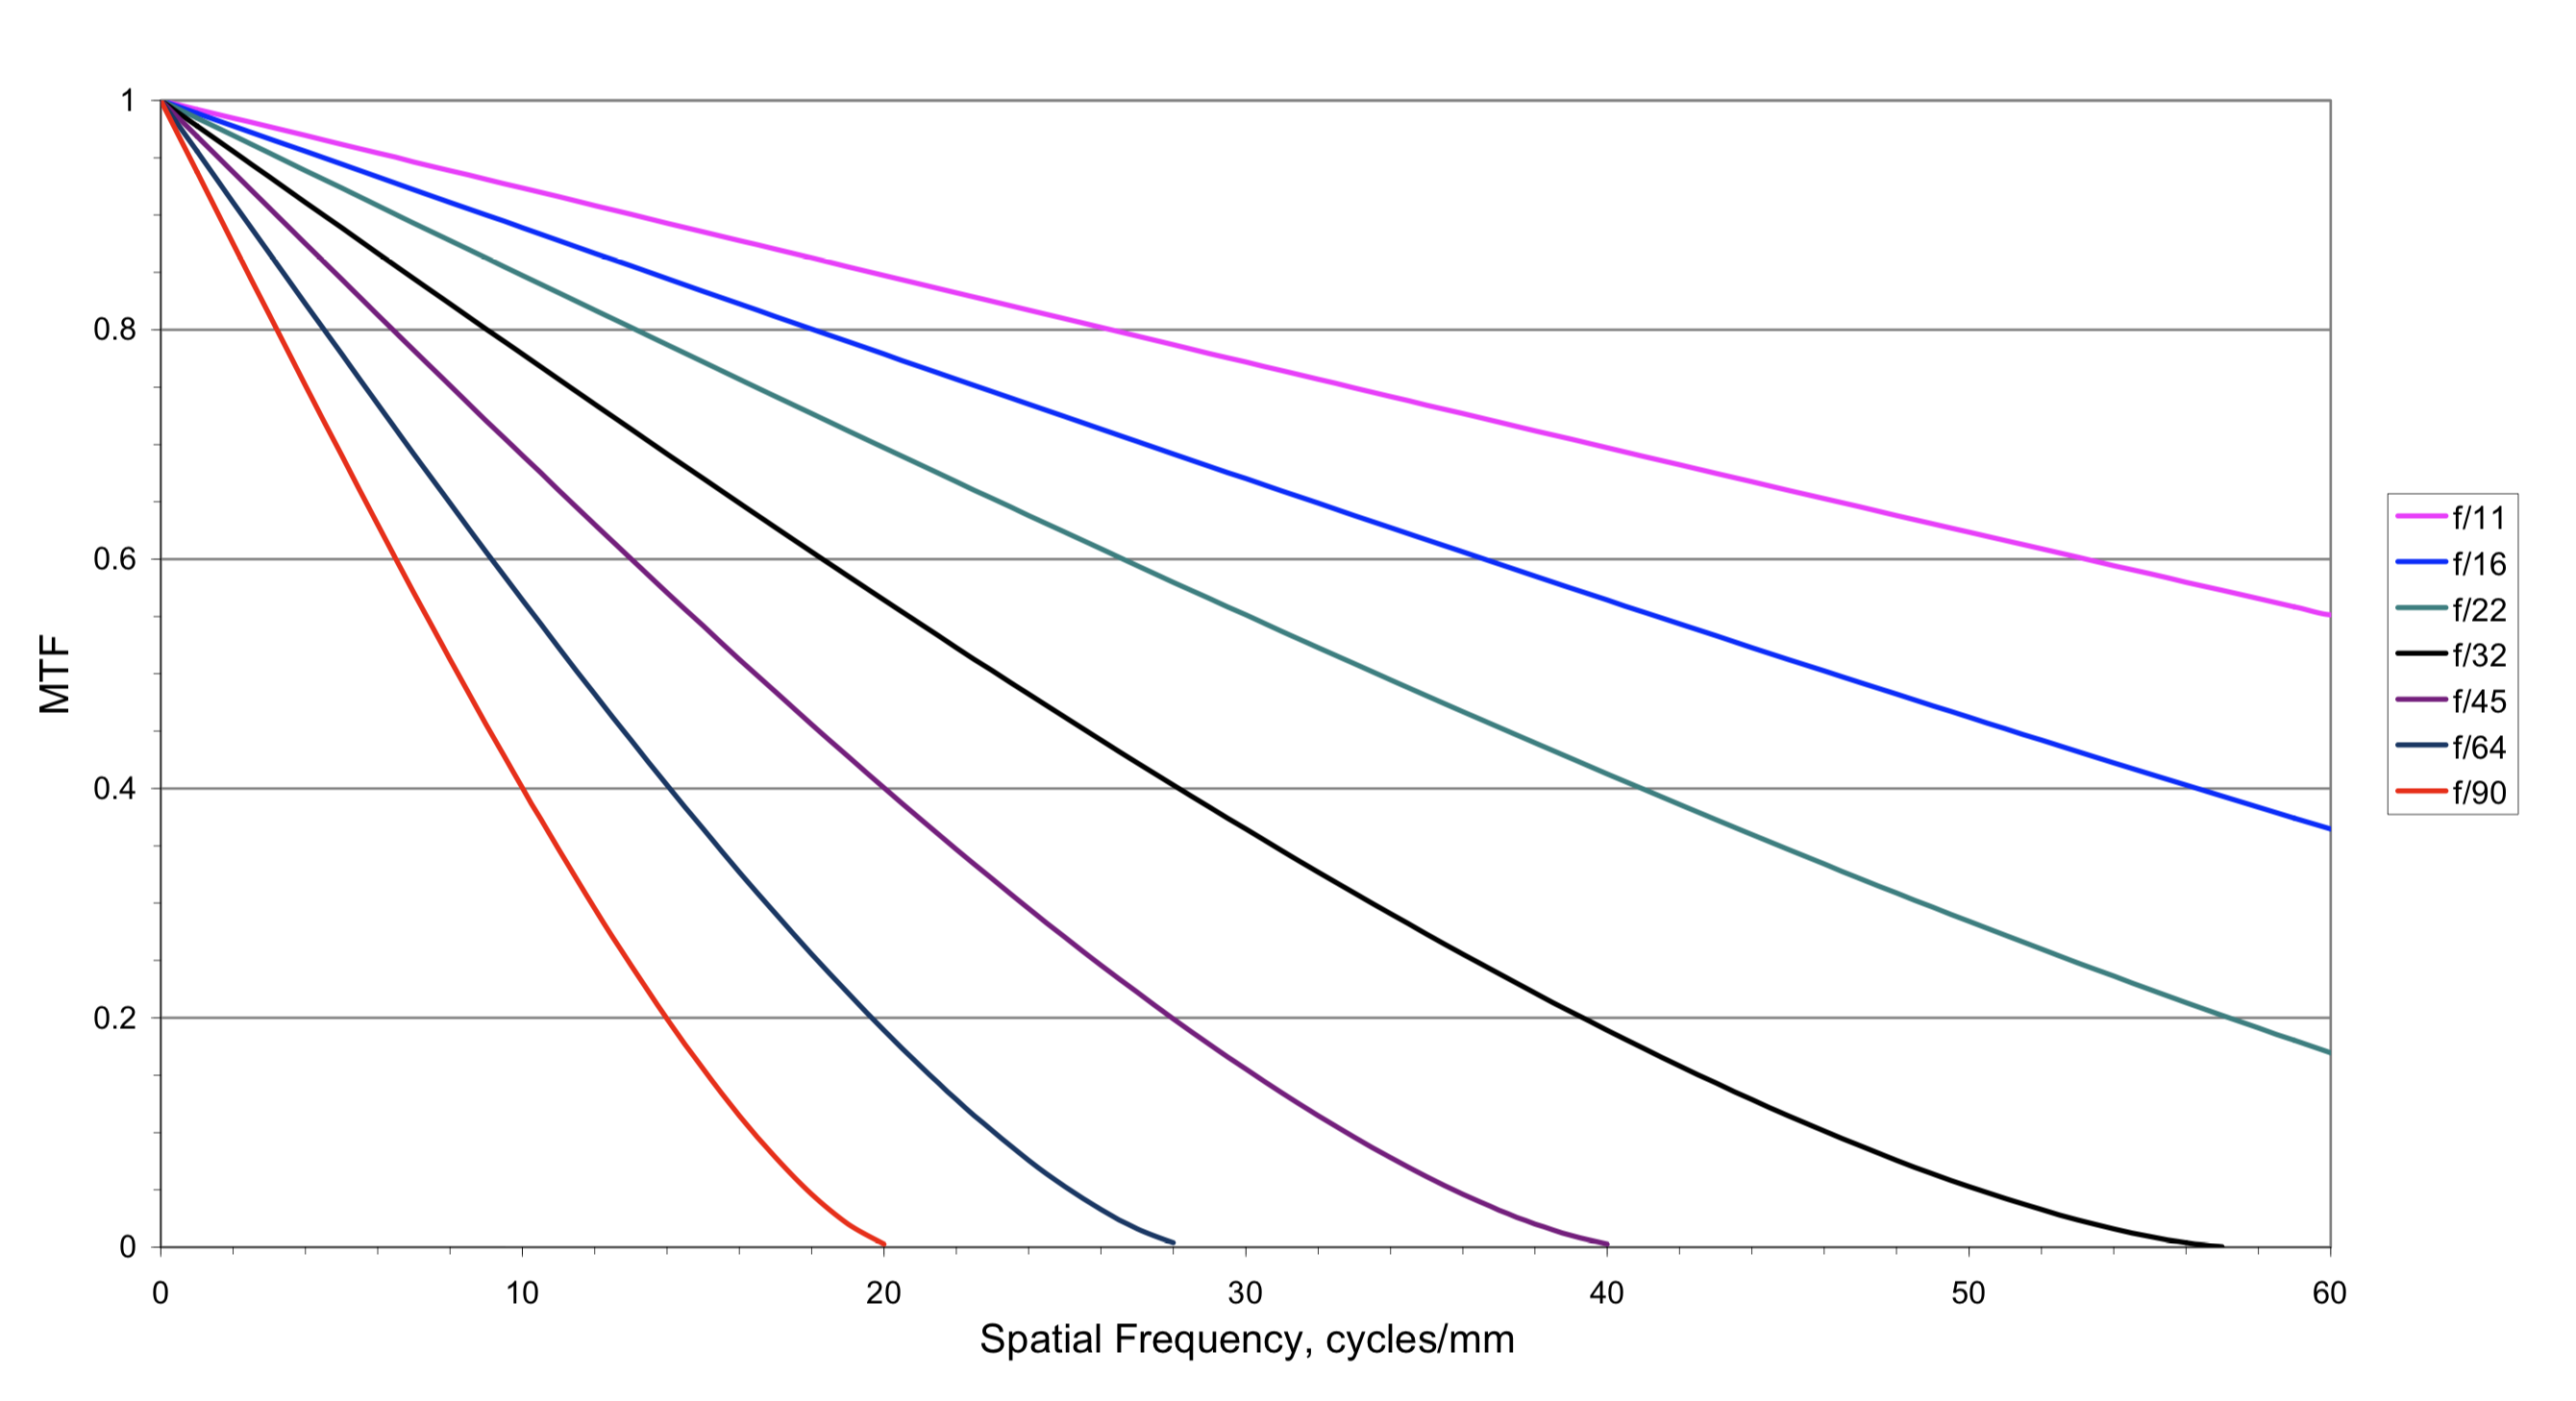
\includegraphics[width=\linewidth]{figure/fig_dofd_6} 
   \caption{MTF for Diffraction-Limited Lens, 4×5, at Various $f$-Numbers}
   \label{fig:MTF}
\end{figure}
%% Figure 6. MTF for Diffraction-Limited Lens, 4×5, at Various $f$-Numbers
Diffraction acts as a low-pass filter, leading to blurring of fine detail. As the $f$-number is increased by stopping down, the blurring occurs at progressively lower spatial frequencies. The spatial frequency corresponding to the Rayleigh criterion is given by Eq. (109); at that frequency, the MTF given by Eq. (115) is approximately 0.09. Eq. (115) is zero when $\phi = 0$, corresponding to
\begin{equation}
   v_0 = \frac1{\lambda N(1+m)}
   \label{eq:v0}
   % #116
\end{equation}
sometimes called the cutoff spatial frequency because it is the maximum spatial frequency that a lens will transmit. This frequency is the same as that corresponding to the Dawes resolution criterion. For $λ = 546$\,nm, at infinity focus,
\begin{equation}
   v_0 \approx \frac{1830}N\,\mathrm{lp/mm}\quad.
   \label{eq:v0num}
\end{equation}                                
A method for determining the MTF for a diffraction-limited lens with defocus was developed by Hopkins (1955):
\begin{equation}
   \mathrm{MTF}(k,N,v) = \frac4{\pi a}\int_0^{\sqrt{1-s^2}}\sin \left[a\left(\sqrt{1-y^2} - s \right) \right] dy \quad,
   % # (117)
   \label{eq:MTF}
\end{equation}
where
\begin{equation}
 a = πv k
\end{equation}
and $s$ is the normalized spatial frequency\footnote{Hopkins specified $s = 2λvN(1 + m)$, giving a range of 0--2 rather than 0--1.} given by
\begin{equation}
s = v/v_0 \stackrel{{\tiny (\ref{eq:v0})}}{= }λvN(1+m)
\end{equation}
It can be shown (Hopkins 1955; Williams and Becklund 1989) that the result is a converging series of Bessel functions of the first kind; however, for most practical applications, direct numerical integration of Eq. (117) is easier. Eqs. (115), (117), and (118) were described by Jacobson (1992) in his classic lens tutorial.

Diffraction sometimes can be ignored when defocus is sufficiently great or the $f$-number sufficiently small. The MTF for a defocused lens considering only geometrical optics is
\begin{equation}
   \mathrm{MTF}(k,v)= \frac{2J_1(a)}a\quad,
   % # (118)
\end{equation}
where $J_1(\cdot)$ is the first-order Bessel function of the first kind.

For any particular image, the photographer’s requirements establish the required DoF, and consequently, the focus spread. If appropriate camera movements have been employed, the only control available to the photographer is the $f$-number. Consider, for example, a 4×5 image for which the focus spread is 5\,mm. Using the standard CoC of 0.1\,mm, the $f$-number from Eq. (39) is
\begin{equation}
N = \frac5{2×0.1} = 25\quad; 
\end{equation}
%% 
the results of this setting are shown in Fig.~\ref{fig:MTFvssf25}.
\begin{figure}[htbp] %  figure placement: here, top, bottom, or page
   \centering
   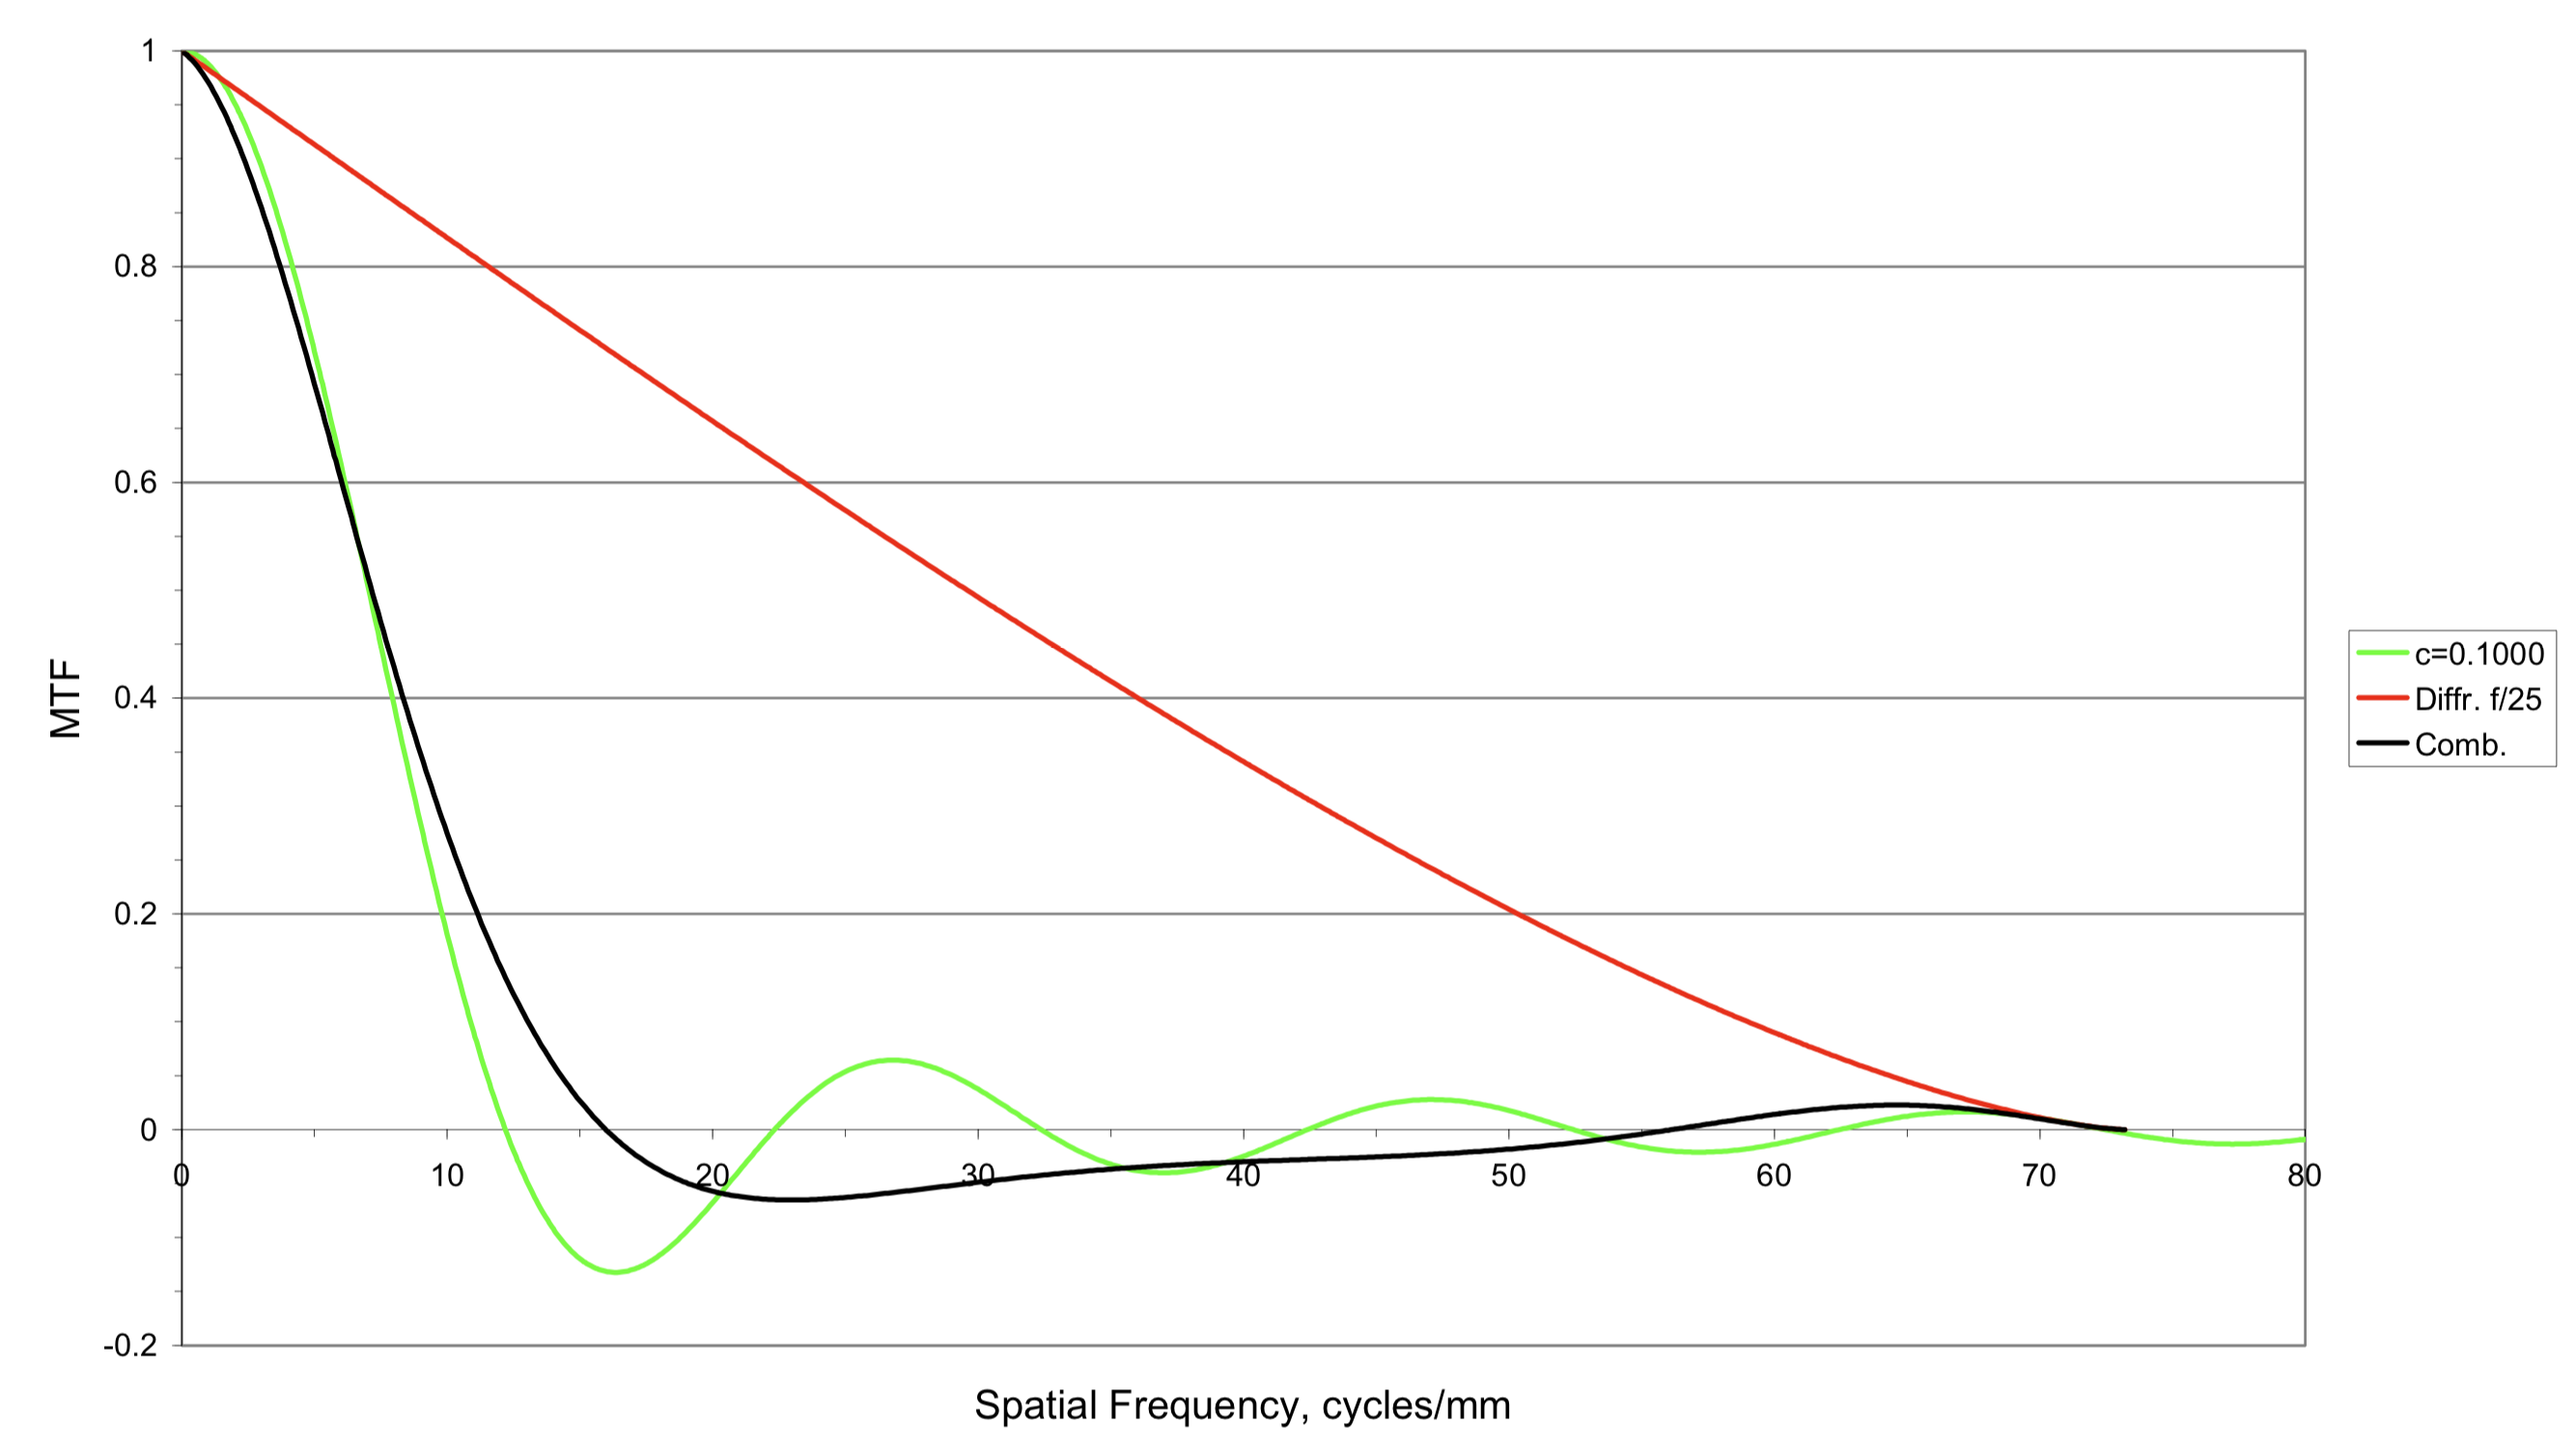
\includegraphics[width=\linewidth]{figure/fig_dofd_7} 
   \caption{MTF vs. Spatial Frequency, 5\,mm Focus Spread at \f{25}}
   \label{fig:MTFvssf25}
\end{figure}
%% Figure 7. MTF vs. Spatial Frequency, 5\,mm Focus Spread at f/25
Three curves are shown: the MTF at \f{25} with no defocus, using Eq. (115), corresponding to the plane of focus; the MTF for the diffraction with defocus, using Eq. (117), corresponding to the DoF limits; and the MTF for a blur spot of 0.1\,mm, ignoring diffraction, using Eq. (118). The negative values of the MTF indicate spurious resolution arising from phase shift; when the MTF is less than zero, light and dark are inverted. The first zero for a pure defocus blur spot would occur at a spatial frequency of approximately $1.22/k$; at a spatial frequency equal to $1/k$, the MTF would be approximately 0.2, so the CoC corresponds to a spatial frequency with an MTF of 0.2. The curve for pure defocus represents a hypothetical situation; although it is possible to have diffraction without defocus, it is not possible to have defocus without diffraction.

There is no standard way to relate an MTF to a single value for resolving power, but a reasonable approach might be to use the spatial frequency corresponding to the CoC, which occurs at an MTF of 0.2. In Figure 7, this frequency is approximately 11\,cycles/mm, just meeting the CoC criterion of 10\,lp/mm, as might be expected. The MTF at the DoF limits is dominated by the effect of defocus; the resolving power from the diffraction-limited MTF at the plane of focus is approximately 50\,lp/mm.

\begin{figure}[htbp] %  figure placement: here, top, bottom, or page
   \centering
   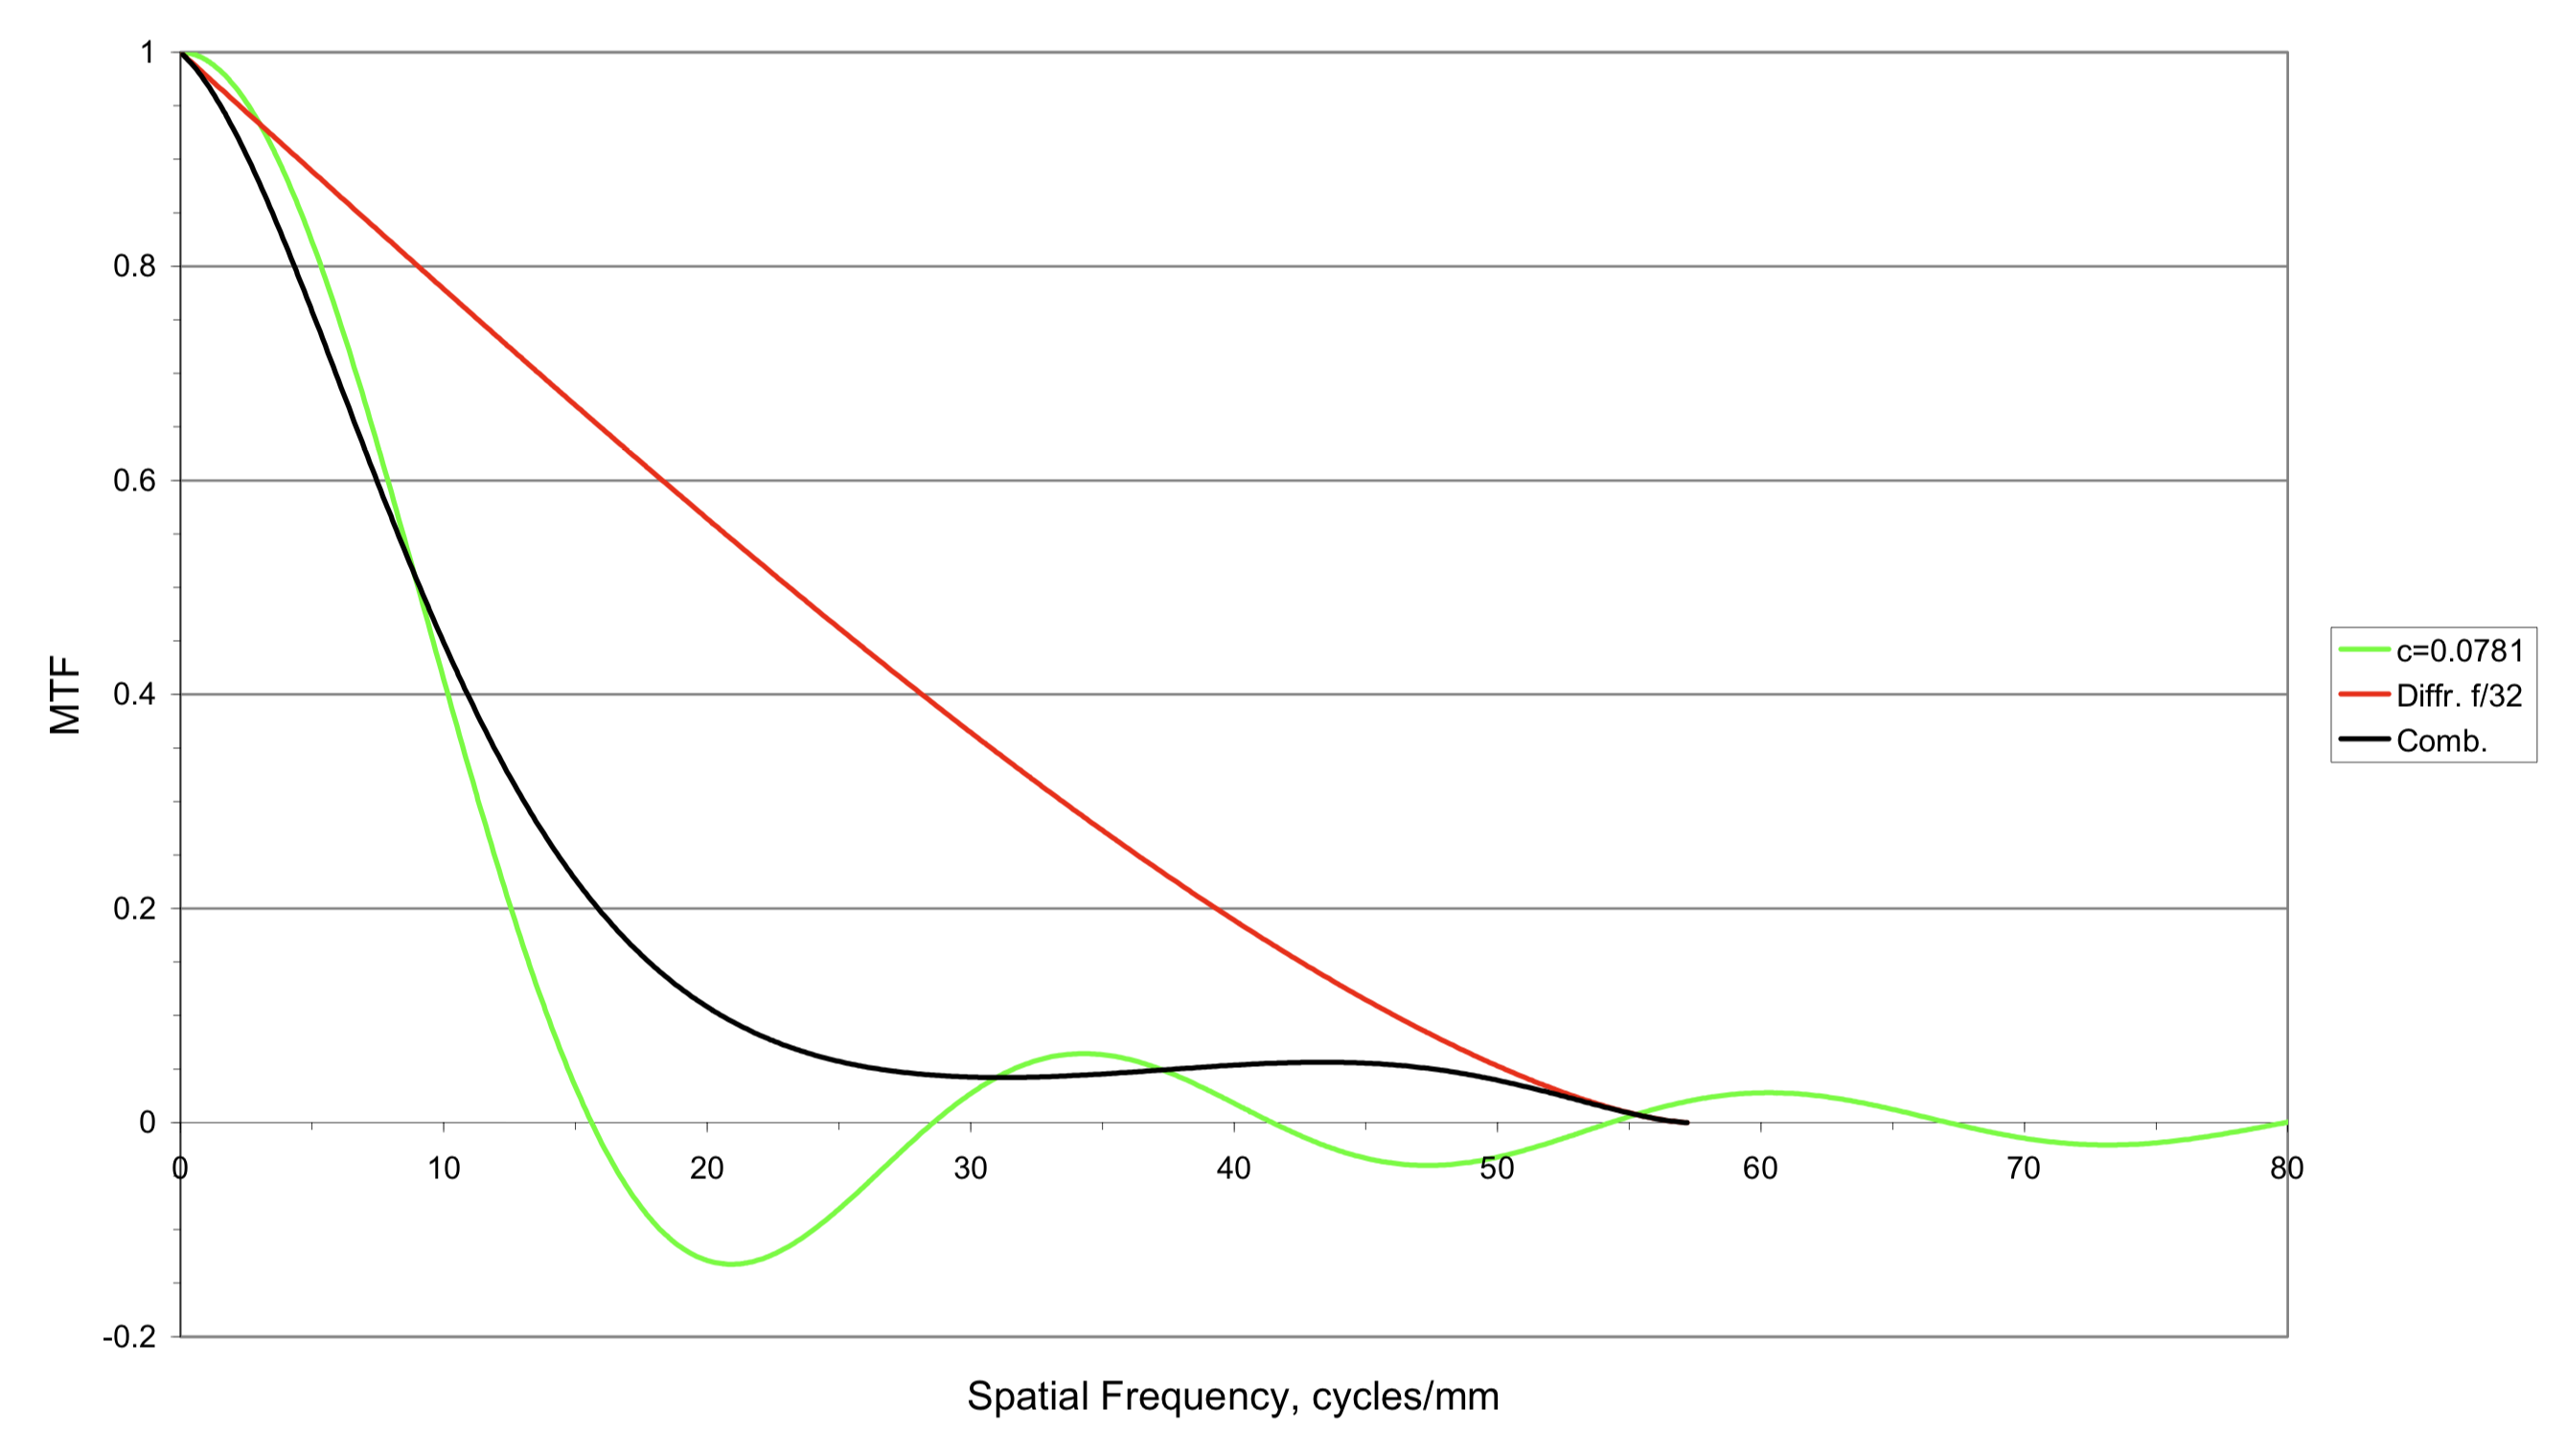
\includegraphics[width=\linewidth]{figure/fig_dofd_8} 
   \caption{MTF vs. Spatial Frequency, 5\,mm Focus Spread at \f{32}}
   \label{fig:MTFvssf32}
\end{figure}
%% Figure 8. MTF vs. Spatial Frequency, 5\,mm Focus Spread at f/32
Rather than set \f{25}, a photographer well might round up to \f{32}; the results of doing so are shown in Figure 8; a change of 1⁄3 step brings noticeable changes. The resolving power at the DoF limits increases to about 16\,lp/mm, while that at the plane of focus decreases to approximately 40\,lp/mm. Additionally, the composite MTF is greater than zero for all spatial frequencies less than the cutoff.

\begin{figure}[htbp] %  figure placement: here, top, bottom, or page
   \centering
   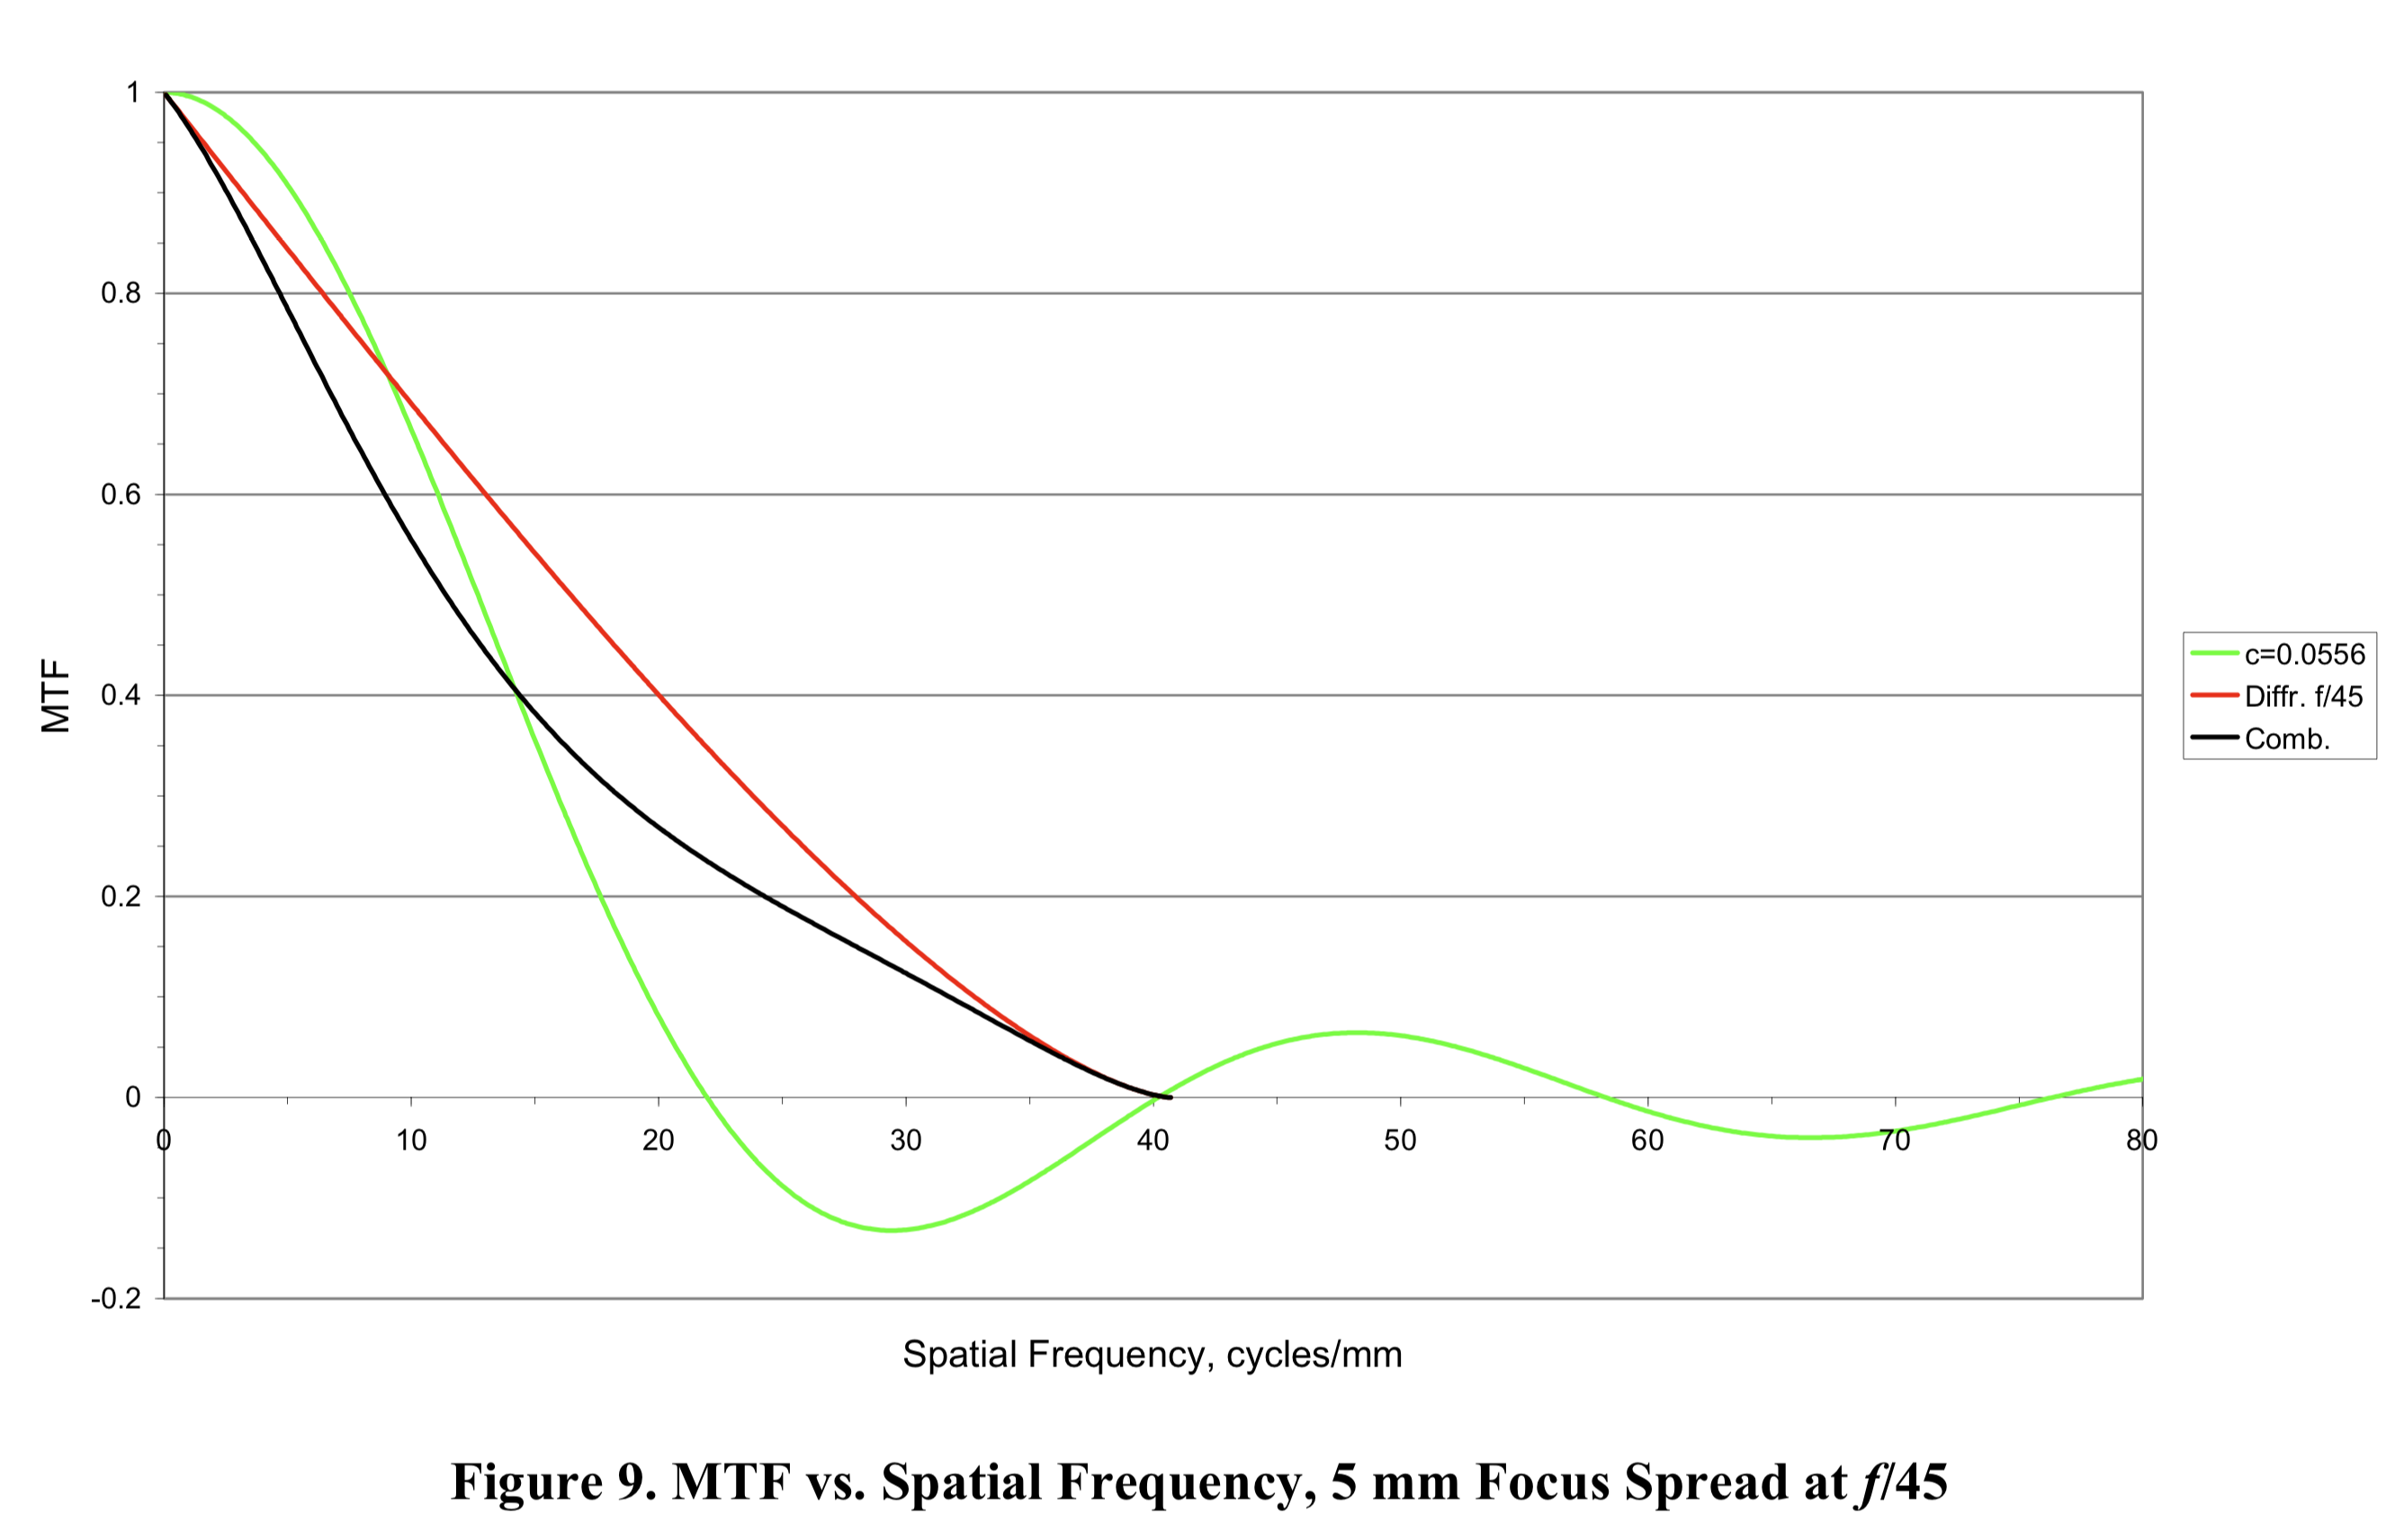
\includegraphics[width=\linewidth]{figure/fig_dofd_9} 
   \caption{MTF vs. Spatial Frequency, 5\,mm Focus Spread at \f{45}}
   \label{fig:MTFvssf45}
\end{figure}
%% Figure 9. MTF vs. Spatial Frequency, 5\,mm Focus Spread at f/45
Increasing the $f$-number to 45 brings a significant change to the shape of the curve, as shown in Figure 9; the effects of defocus and diffraction now appear nearly equal. The resolving power at the DoF limits increases to 24\,lp/mm, and that at the plane of focus decreases to 28\,lp/mm.

\begin{figure}[htbp] %  figure placement: here, top, bottom, or page
   \centering
   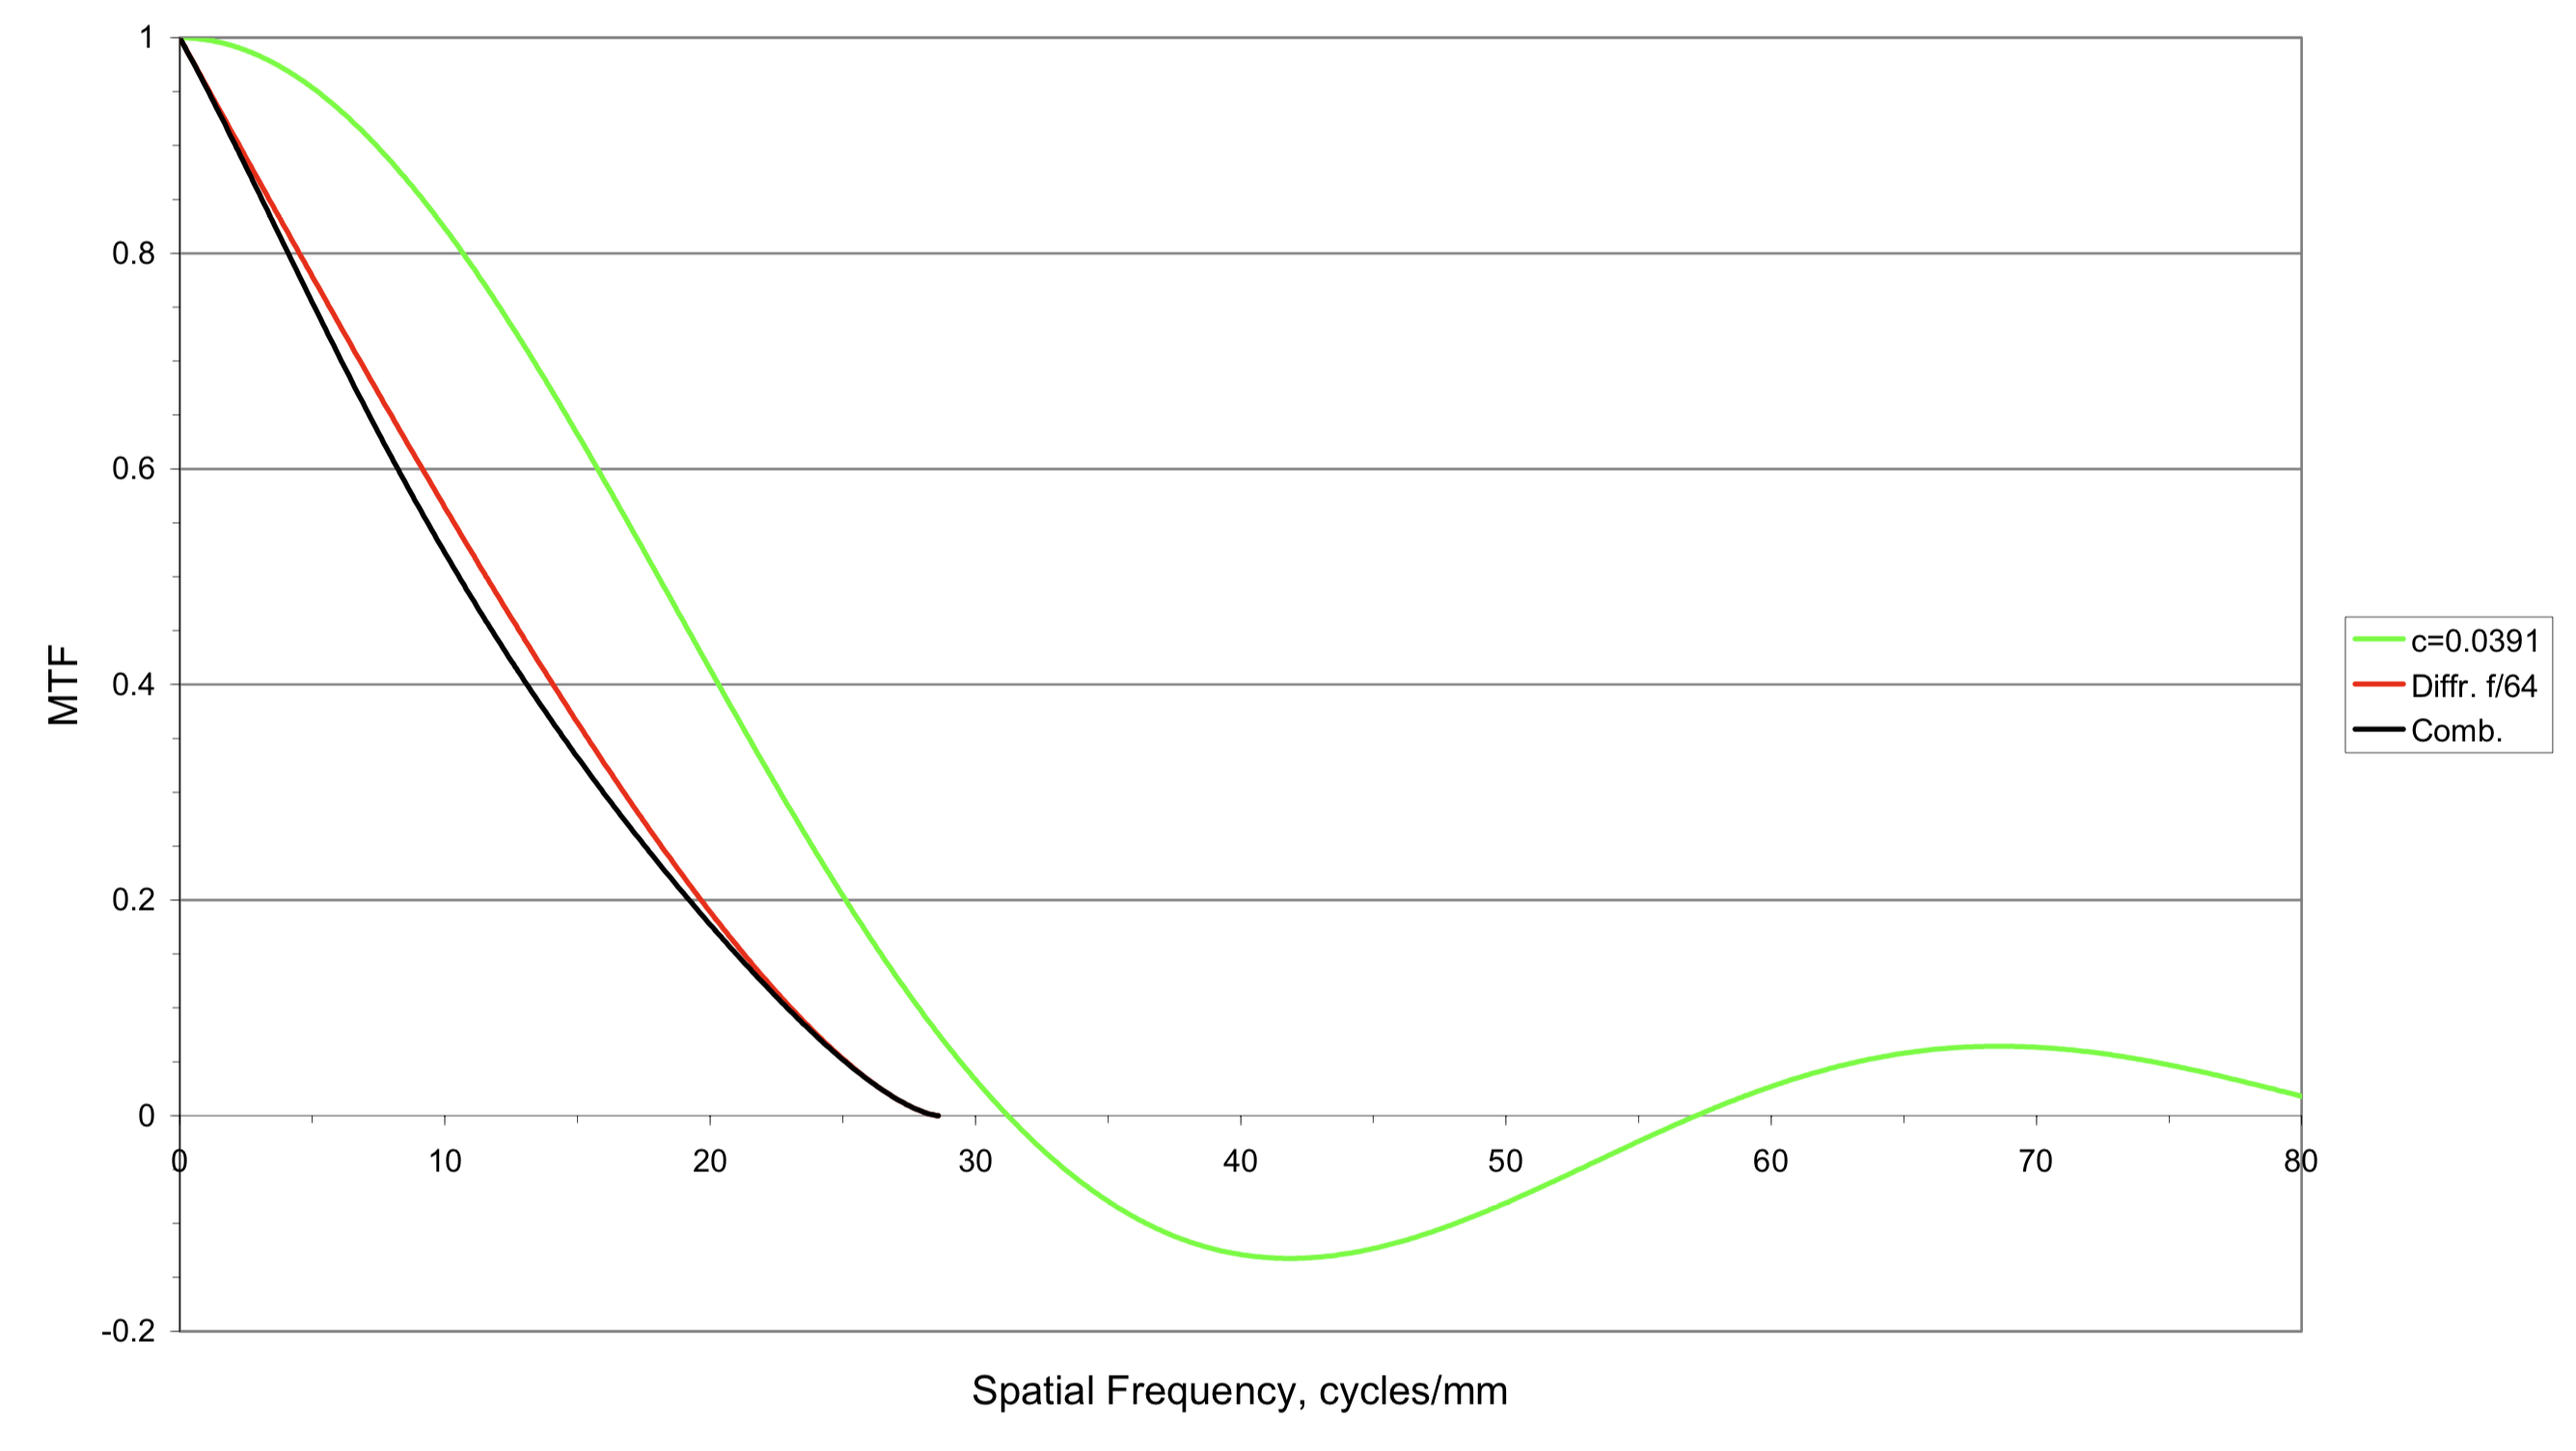
\includegraphics[width=\linewidth]{figure/fig_dofd_10} 
   \caption{MTF vs. Spatial Frequency, 5\,mm Focus Spread at \f{64}}
   \label{fig:MTFvssf64}
\end{figure}
%% Figure 10. MTF vs. Spatial Frequency, 5\,mm Focus Spread at f/64
Eventually, stopping down fails to give improvement. If the $f$-number is increased to 64, the
MTF is dominated by diffraction. The resolving power decreases to 19\,lp/mm and that at the 
plane of focus decreases to 20\,lp/mm. Clearly, much better results are obtained with \f{45} than with \f{64}.
\subsection{Optimum $f$-Number from MTF}

The results in Figure 7 through Figure 10 suggest that, for a given focus spread and spatial frequency, there is an optimum $f$-number for the DoF limits. This perhaps can be better illustrated by plotting MTF vs. $f$-number for different spatial frequencies at various focus spreads, as shown in Fig.~\ref{fig:MTFvsf3} and Fig.~\ref{fig:MTFvsf10}.
\begin{figure}[htbp] %  figure placement: here, top, bottom, or page
   \centering
   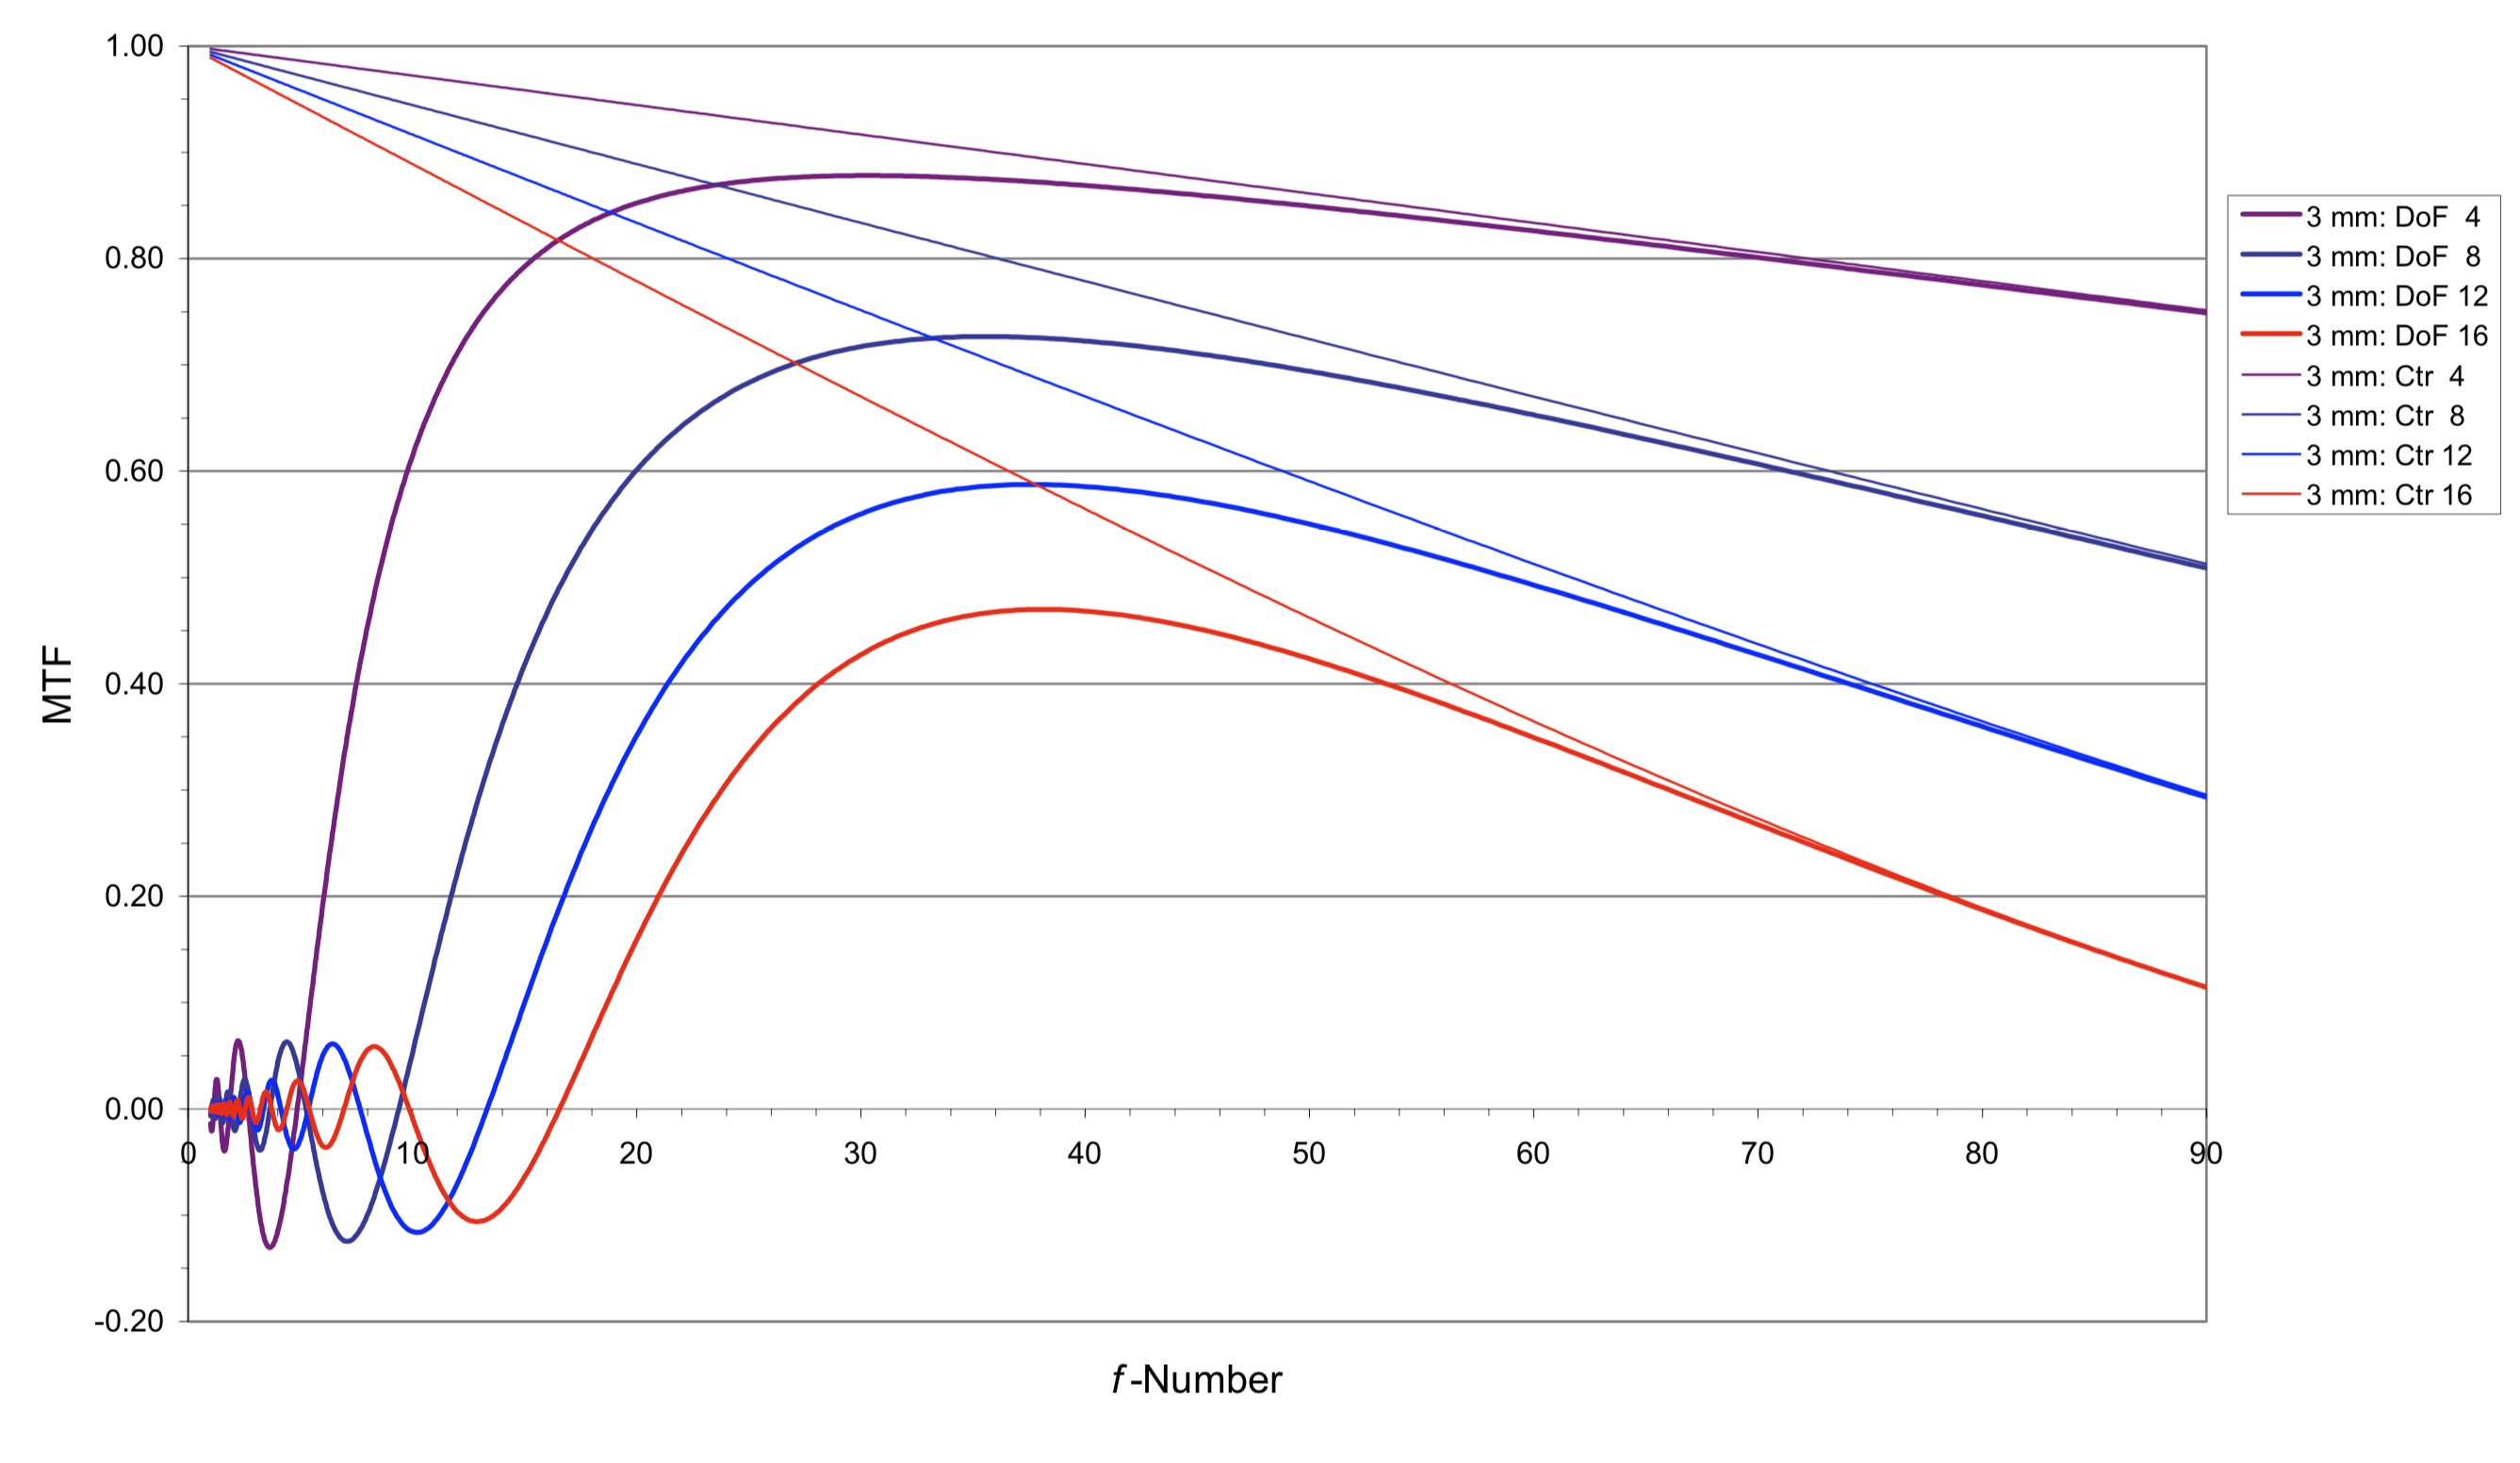
\includegraphics[width=\linewidth]{figure/fig_dofd_11} 
   \caption{MTF vs. $f$-Number: 4×5, 3\,mm Focus Spread}
   \label{fig:MTFvsf3}
\end{figure}
%% Figure 11. MTF vs. $f$-Number: 4×5, 3\,mm Focus Spread

\begin{figure}[htbp] %  figure placement: here, top, bottom, or page
   \centering
   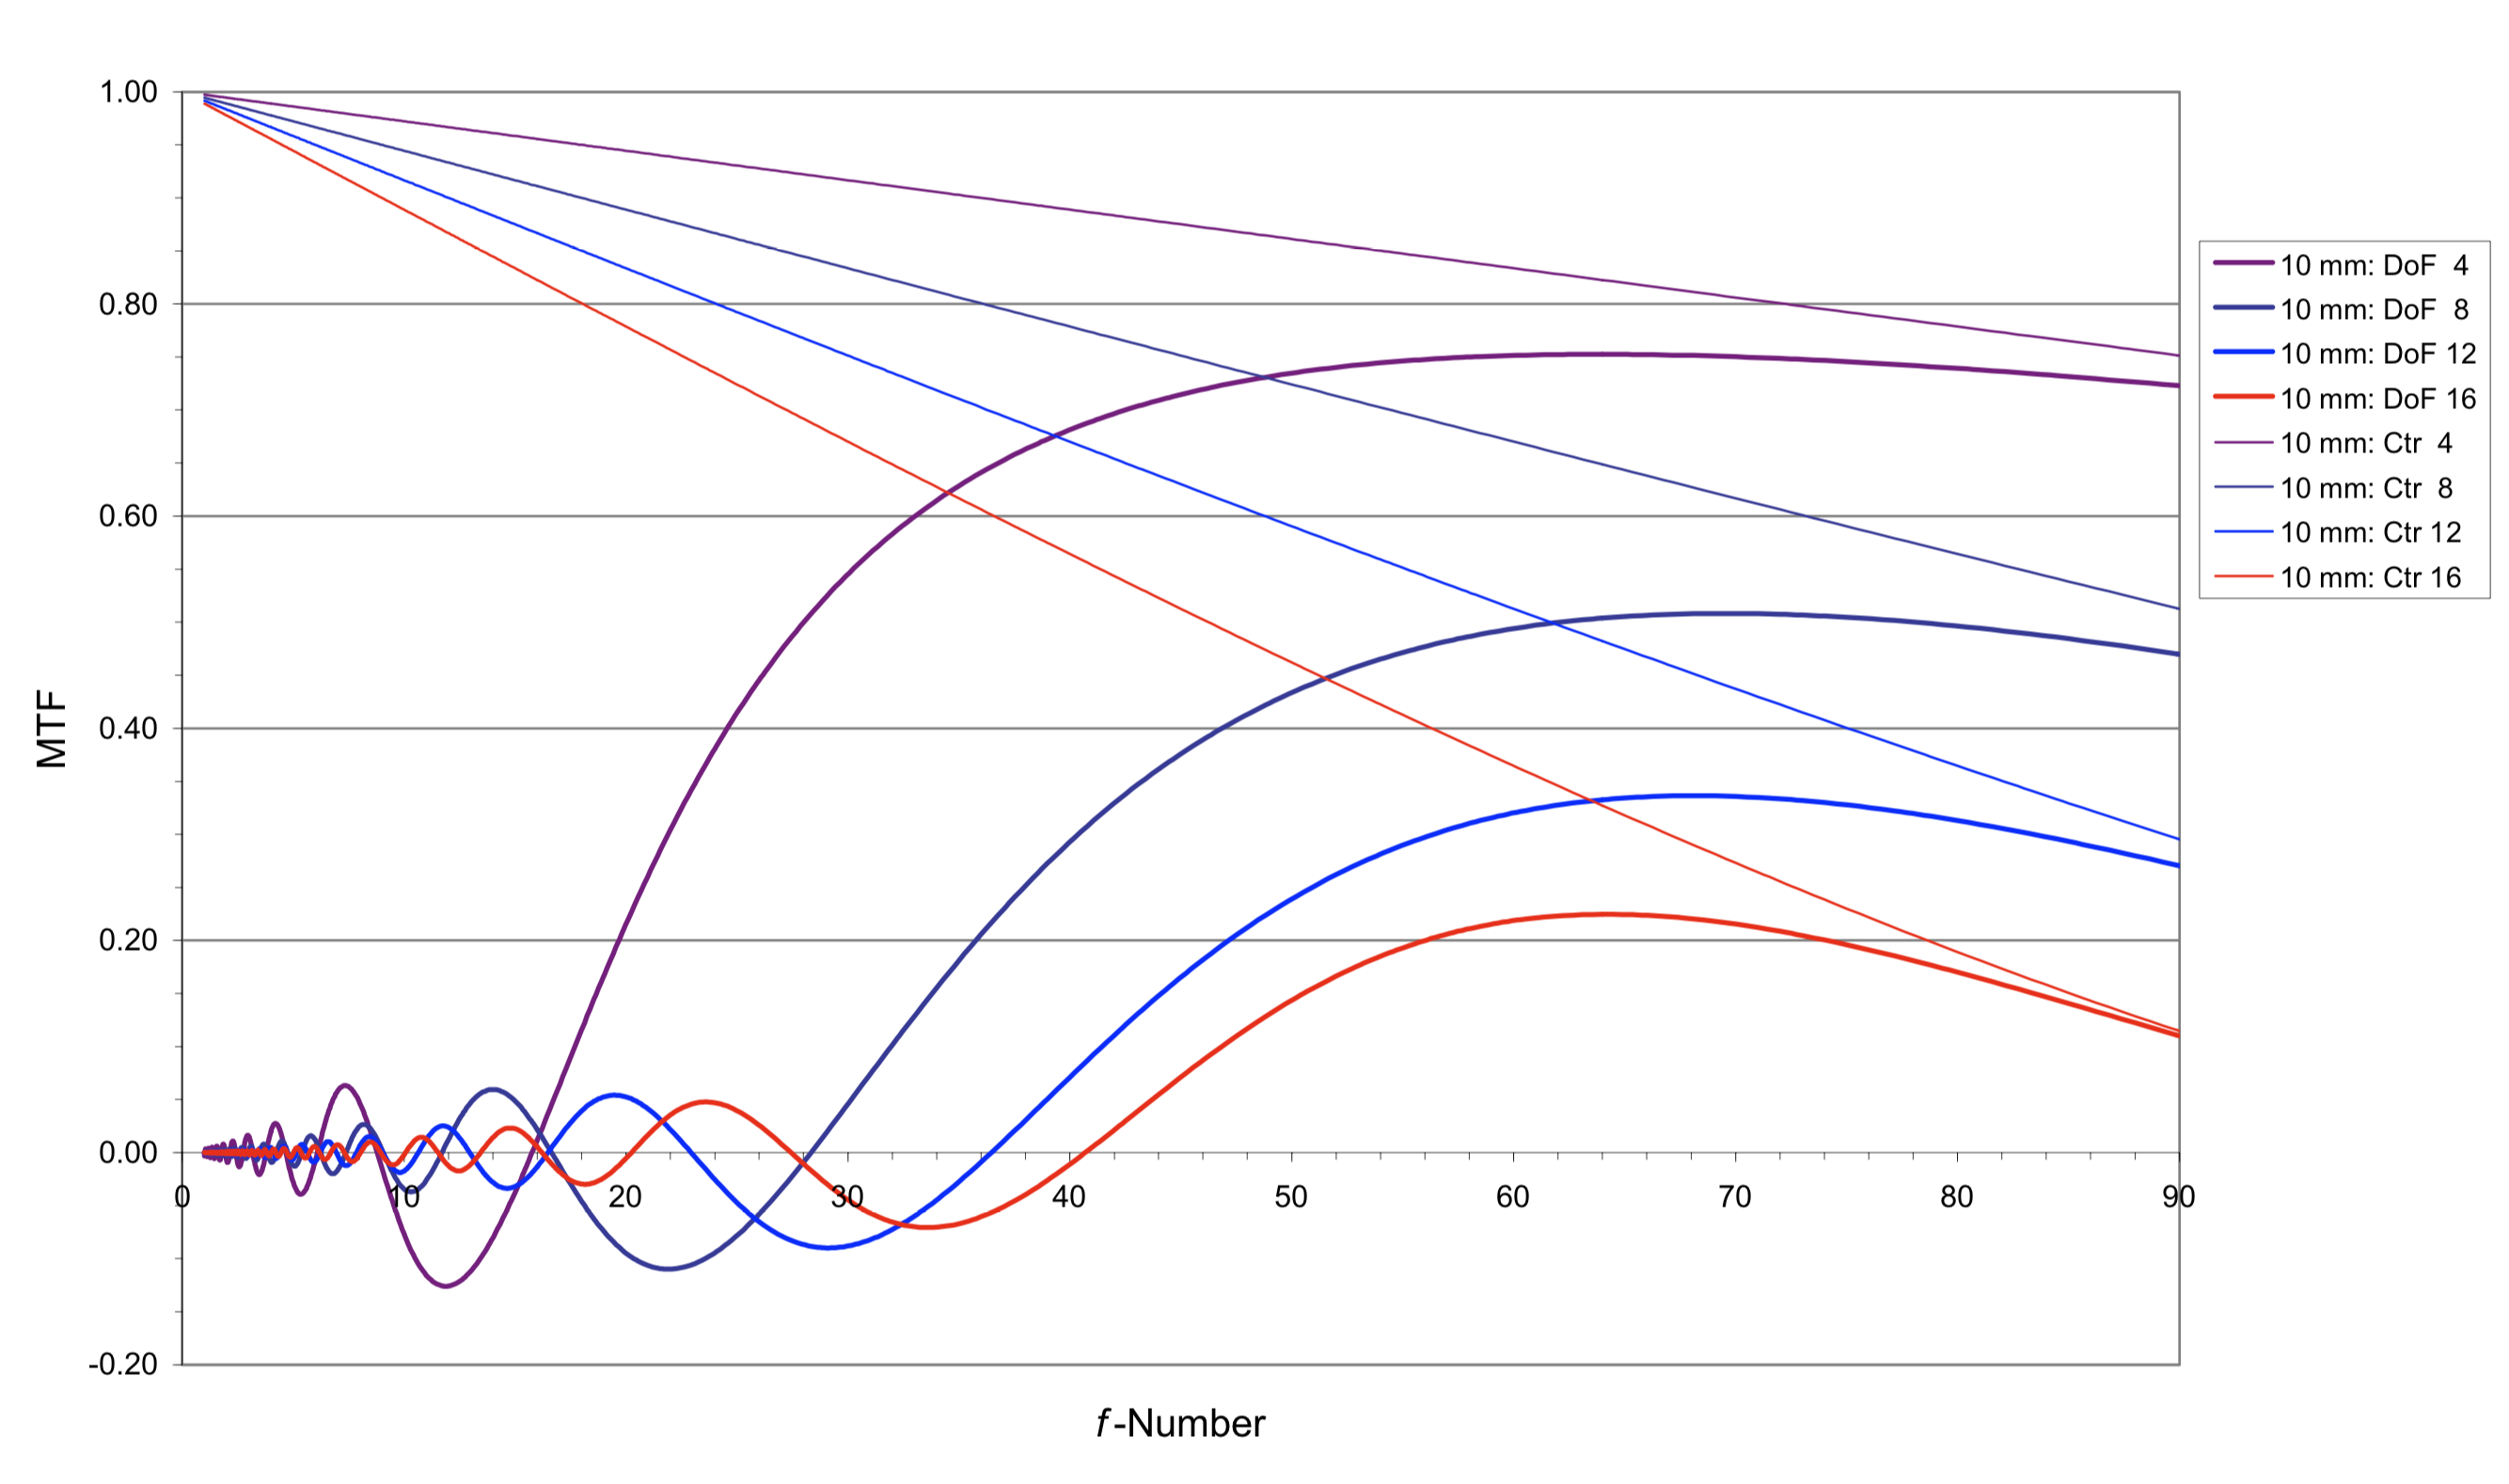
\includegraphics[width=\linewidth]{figure/fig_dofd_12} 
   \caption{MTF vs. $f$-Number: 4×5, 10\,mm Focus Spread}
   \label{fig:MTFvsf10}
\end{figure}
%% Figure 12. MTF vs. $f$-Number: 4×5, 10\,mm Focus Spread
Eight curves are shown in each figure: four for diffraction alone, and four for diffraction with defocus. The thin lines labeled ‘$m$ mm: Ctr $n$’ are for diffraction, and correspond to the plane of focus; the bold lines labeled ‘$m$ mm: DoF $n$’ are for diffraction with defocus, and correspond to the limits of DoF. In each case, curves are shown for spatial frequencies of 4, 8, 12, and 16 lp/mm. Assuming a 2× enlargement, they correspond to spatial frequencies of 2, 4, 6, and 8 lp/mm in the final image; 2 lp/mm relates to perception of contrast in coarse detail, and 6 and 8 lp/mm relate to perception of sharpness in fine detail.

The conventionally determined $f$-number for a 3\,mm focus spread is 
\begin{equation}
N = \frac{3\,\mathrm{mm}}{2\times 0.1\,\mathrm{mm}} = 15
\end{equation}
In Fig.~\ref{fig:MTFvsf3}, the negative value of the MTF for 16 lp/mm at f/15 suggests spurious resolution in some fine detail, although this arguably would be near the threshold of visibility in the final image and might not be obvious.

As can be seen, the optimum $f$-number is different for each spatial frequency, although the values tend to converge at large focus spreads. As focus spread increases, the optimum $f$-number increases and MTF at the optimum $f$-number decreases for all spatial frequencies. At any given focus spread, as $f$-number is increased, the defocus blur spot decreases while the diffraction blur spot increases. The defocus blur spot eventually approaches zero, so the effect of diffraction becomes dominant, and the MTF asymptotically approaches the MTF from diffraction alone.

Fitting power functions to the calculated optimum $f$-numbers for focus spreads up to 16\,mm gives
\begin{eqnarray}
N_4 &=&15.1(\Dv)^{0.62}\\
N_8 &=&18.8(\Dv)^{0.57}\\
N_{12} &=&21.0(\Dv)^{0.51}\\
N_{16} &=&22.4(\Dv)^{0.45}
\end{eqnarray}
for the optimum $f$-numbers at 4, 8, 12, and 16\,lp/mm.

Interestingly, the equation fit to 12 \,lp/mm, corresponding to 6\,lp/mm in the final image,
is close to that for Hansma’s method for optimum $f$-number, using Eq. (114) with $K_\lambda = 883$. Fig.~\ref{fig:MTFvsf3} and Fig.~\ref{fig:MTFvsf10} are difficult to compare with the graph of Hansma’s values shown in Figure 5. To derive a single sharpness value from an MTF, it is necessary to select a spatial frequency corresponding to a particular value of MTF. Again taking an MTF of 0.2 as indicative of resolving power, the optimum $f$-numbers from calculated MTFs are shown in Figure~\ref{fig:respow}.

\begin{figure}[htbp] %  figure placement: here, top, bottom, or page
   \centering
   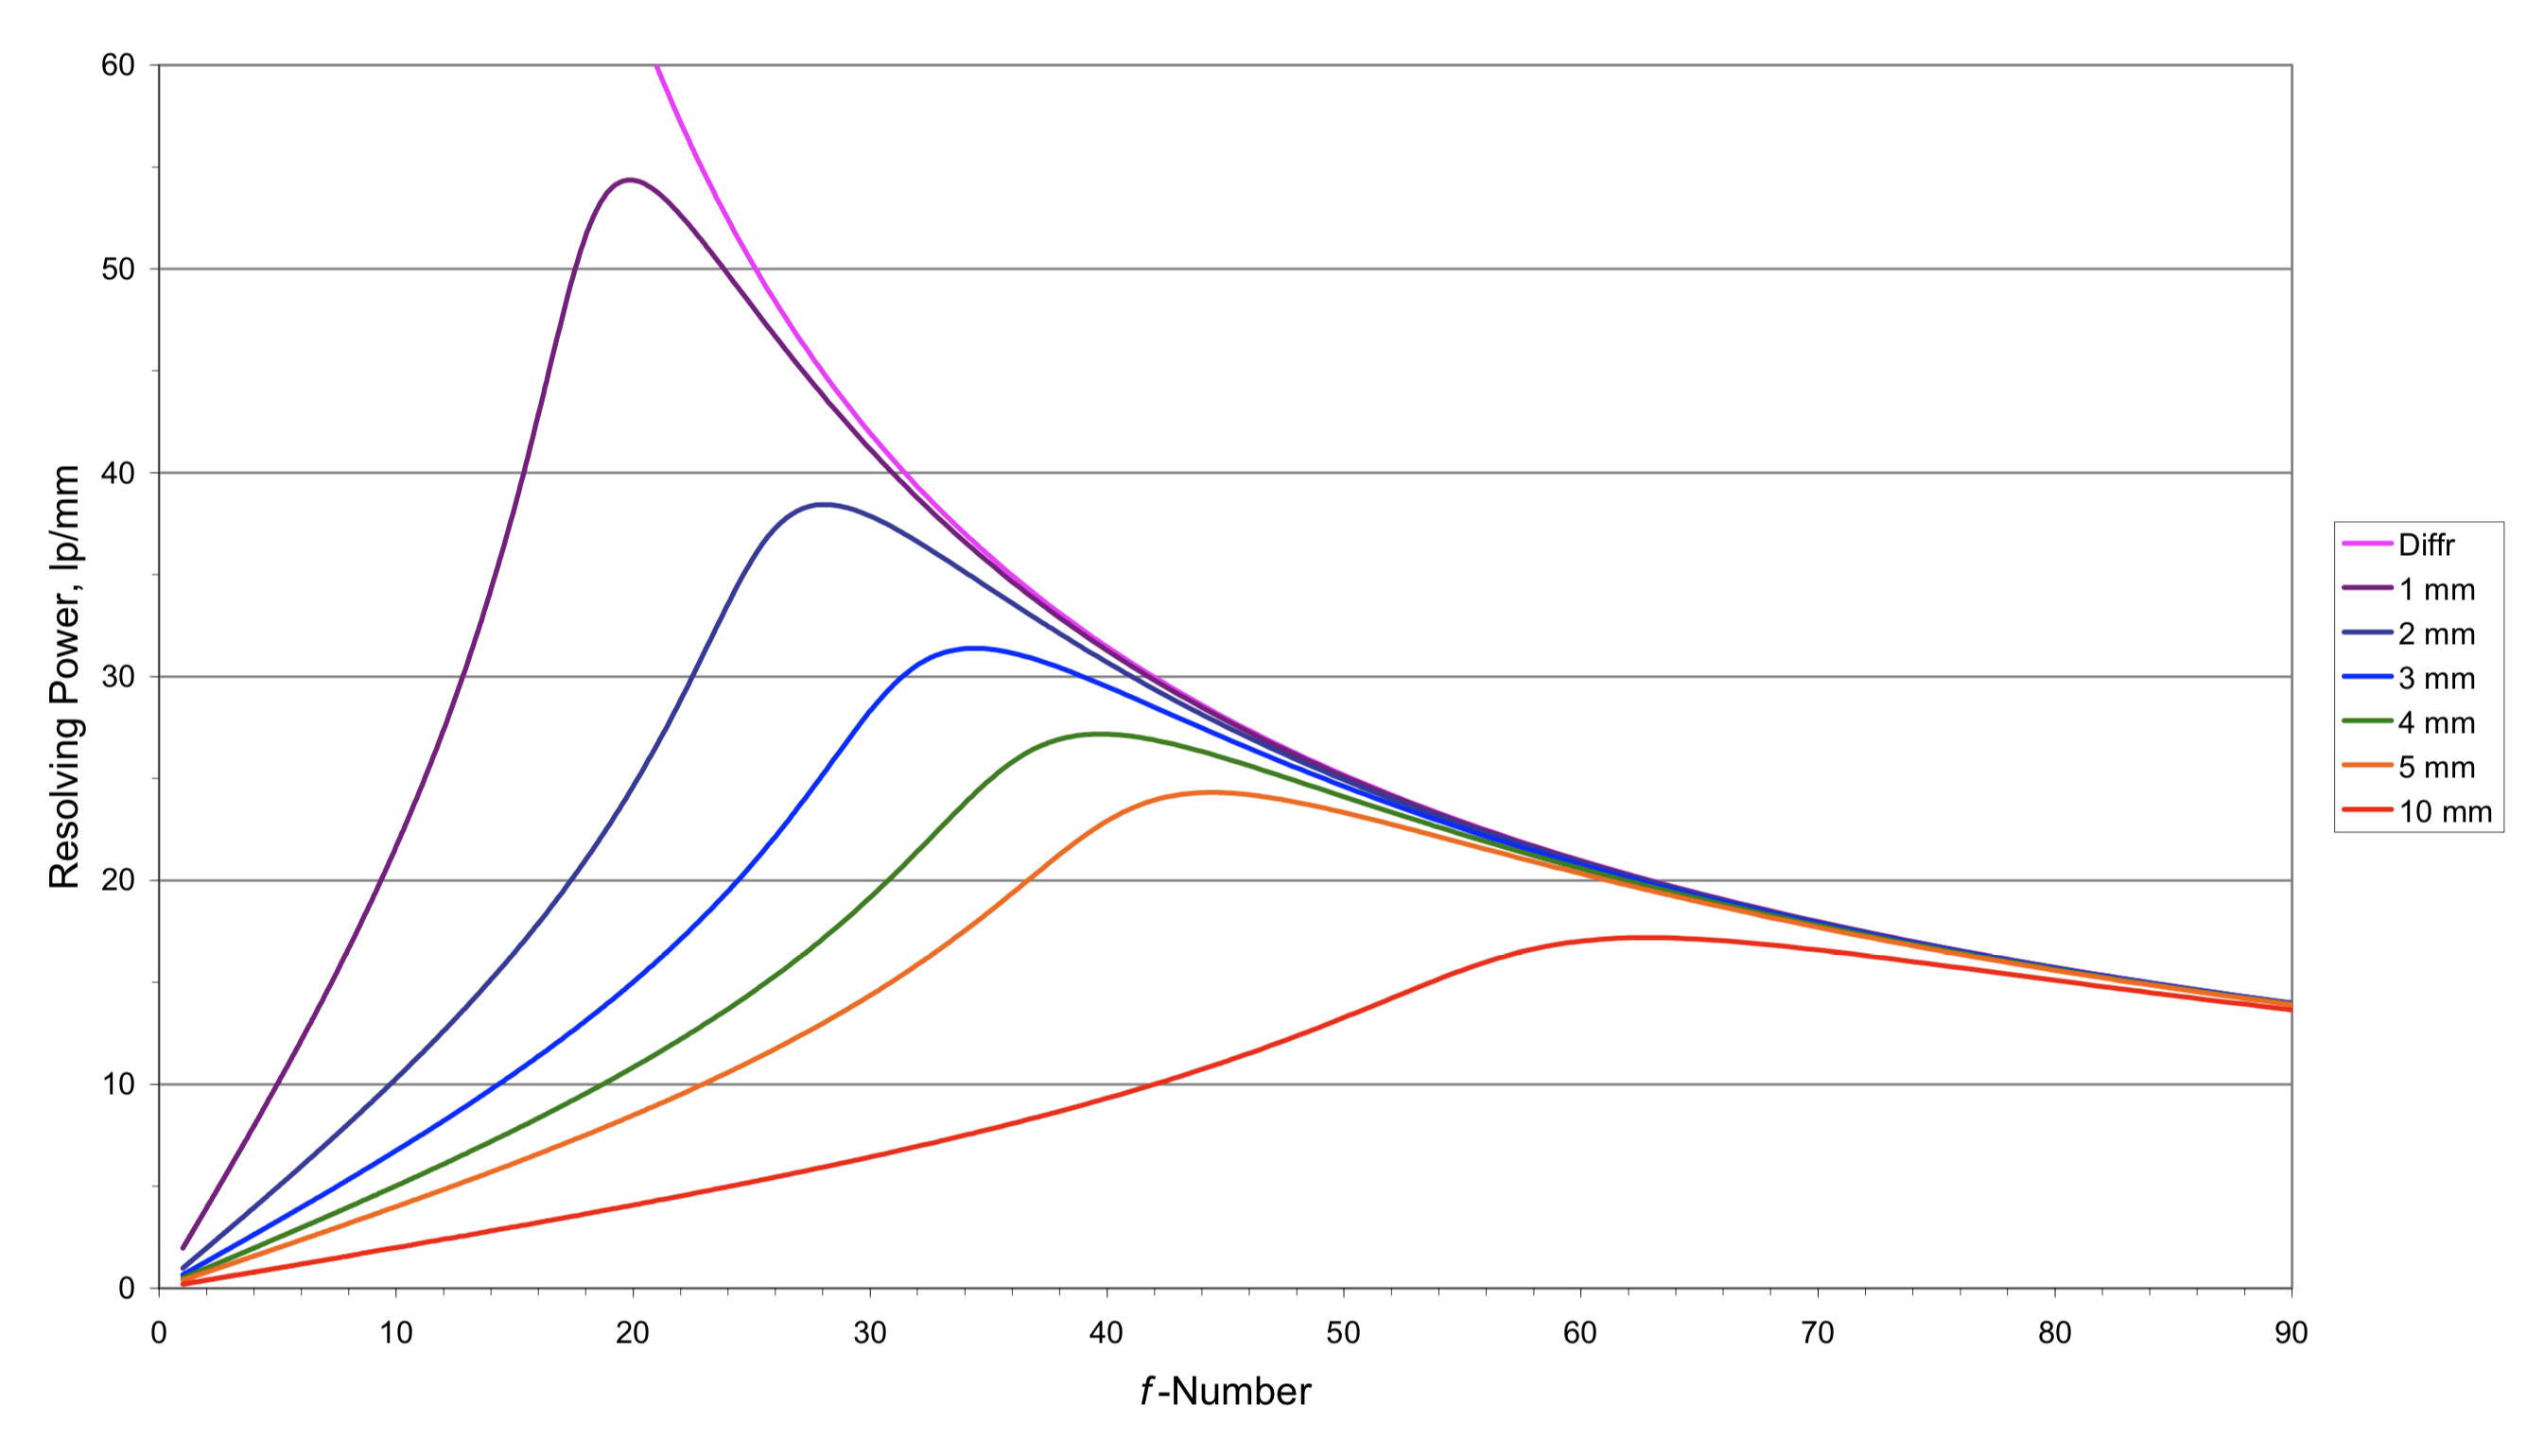
\includegraphics[width=\linewidth]{figure/fig_dofd_13} 
   \caption{Resolving Power vs.\ $f$-Number at Various Focus Spreads---from MTF}
   \label{fig:respow}
\end{figure}
%% Figure 13. Resolving Power vs. $f$-Number at Various Focus Spreads—from MTF

The curves exhibit sharper peaks than those in Figure 5, although the optimum $f$-numbers and corresponding resolving powers are essentially the same. The values at the diffraction limit are different because Figure 13 uses the CoC criterion rather than the Rayleigh criterion; if the Rayleigh criterion is to determine resolving power, the correspondence to Hansma’s model of the curves that include defocus is not nearly as good. A power function fit to the optimum $f$-numbers derived from Figure 13 gives
\begin{equation}
N_{0.2} = 19.8\sqrt{\Dv}\quad,
\end{equation}
quite close to Eq. (114) with $K_\lambda = 787$. Very similar values are obtained if resolving power is determined for MTFs of 0.09 or 0.5, although the curve shapes are substantially different. The fit in all cases is excellent, with the coefficient of determination $r^2$ essentially equal to 1.


These results suggest that a simple formula essentially the same as Hansma’s does quite a good job of predicting optimum $f$-numbers. The different relationships between focus spread and optimum $f$-number for different spatial frequencies also suggest that the “optimum” $f$-number is somewhat arbitrary, and that great precision in the choice of coefficient and exponent is unnecessary. A reasonable compromise might be to take
\begin{equation}
   N_\mathrm{opt} = 20 \sqrt{\Dv}\quad, 
   % #119
   \label{eq:Nopt}
\end{equation}
equivalent to taking $K_\lambda = 800\,\mathrm{mm}^{-1}$. Comparative $f$-numbers for 4$\times$5 ($c = 0.1$\,mm) at infinity focus  ($m = 0$) using the conventional CoC and MTF-optimum methods are shown in Table ~\ref{tab:opt}. 
 \begin{table}[htp]
\caption{Comparison of Conventional and MTF-Optimum Methods}
\begin{center}
\begin{tabular}{|c|c|c|}
\hline
Focus Spread & \multicolumn{2}{c|}{$f$-Number}\\
\cline{2-3}
[mm] & Conventional & MTF-Optimum\\
\hline
\hphantom{0}1 & \hphantom{0}5 & 20.0 \\
\hphantom{0}2 & 10 & 28.3 \\
\hphantom{0}3 &15 & 34.6 \\
\hphantom{0}4 &20 & 40.0 \\
\hphantom{0}5 &25 & 44.7 \\
10 &50 & 63.2 \\
16 & 80 & 80.0 \\
\hline
\end{tabular}
\end{center}
\label{tab:opt}
\end{table}

%%      Focus Spread, mm
%%        $f$-Number
%%      Conventional
%%       MTF-Optimum
%%    1.0 2.0 3.0 4.0 5.0
%% 10.0 16.0
%%         5.0 10.0 15.0 20.0 25.0 50.0 80.0
%%               20.0 28.3 34.6 40.0 44.7 63.2 80.0
The $f$-number from the MTF-optimum method equals that from the conventional approach at zero focus spread and again at
\begin{equation}
  \Dv = 2c^2K_\lambda
  % #120
  \label{eq:DvMTF}
\end{equation}

Between these limits, the MTF-optimum method always gives a greater $f$-number than the conventional method. Table 1 may suggest a combination of the conventional approach and the MTF-optimum method: the $f$-number determined by the conventional approach is the minimum that will give acceptable image sharpness; when other considerations, such as motion blur, permit, increasing the $f$-number will give greater sharpness until the limit given by the MTF-optimum method is reached. The region between the two curves then gives the range of usable $f$-numbers. Recall from Eq. (32) that the focus position is independent of $f$-number, so that the conventional approach for setting focus remains usable.

Eq.~\ref{eq:Nopt} suggests that when the focus spread is greater than the limit given by Eq.~\ref{eq:DvMTF}, the $f$-number should be less than that determined by the conventional method, and that there then is a single value rather than a range of acceptable $f$-numbers. When the limit given by Eq.~\ref{eq:DvMTF} is exceeded, the requirement that the blur spot be smaller than the CoC cannot be met. However, the limit occurs only at large focus spreads: if $c = 0.1$\,mm and $K_λ = 800\,\mathrm{mm}^{-1}$, the limit is at 16\,mm, and the indicated $f$-number is 80.

The MTF-optimum method also implies that, in most practical situations, image degradation from diffraction when determining the $f$-number from the CoC is a comparatively minor concern.

It should be remembered, of course, that both the conventional and
MTF-optimum methods address only the sharpness at the limits of
DoF. At the plane of focus, once a lens essentially is diffraction
limited, any further increase in $f$-number will decrease
sharpness. There is nothing whatsoever to be gained by using an
$f$-number greater than the MTF-optimum value, because the MTF then
decreases at the limits of DoF as well as at the plane of
focus. Accordingly, the MTF-optimum $f$-number is the \emph{maximum} that
should be used. With $\Dv$ in mm, the usable range of
$f$-numbers then is, from Eqs. (39) and \ref{eq:Nopt},
\begin{eqnarray}
   \frac{\Dv}{2c} \leq N \leq 20\sqrt{\Dv}& &\mathrm{for}\quad\Dv<1600c^2 \\
   N = 20\sqrt{\Dv}& &\mathrm{for}\quad\Dv<1600c^2
   % #(121)
   \label{eq:Nusable}  
\end{eqnarray}

When the focus spread is great, there is a considerable loss of sharpness at the plane of focus when setting the maximum $f$-numbers. With a 10\,mm focus spread in 4$\times$5, it simply is not possible to get maximum sharpness. Obviously, anything that can reduce the focus spread, such as the use of camera movements, should be employed.

Conversely, when the focus spread is small, the MTF at the DoF limits using $f$-numbers determined with Eq. (39) is considerably less than optimal. Selection of an $f$-number sometimes involves a tradeoff between the sharpest possible central image and the most uniformly sharp overall image. In many cases, uniform sharpness throughout the image will be preferable to slightly greater sharpness at the plane of focus, but the best choice for any given image will depend on the subject matter. In many situations, the maximum usable $f$-number within the acceptable range will be dictated by consideration of motion blur.

It can be argued that if the blur is less than the threshold of detection, any increase in sharpness is irrelevant; however, having the greatest possible sharpness can be useful if at some time it is decided to make a larger final image than originally planned.

\subsection{Minimum and Maximum $f$-Numbers on Hand-Camera Lenses}
\label{sec:min-max-f}

For a small- or medium-format camera, focus spread usually is difficult to measure, but if the lens manufacturer's CoC is known, the maximum $f$-number can be determined from the $f$-number marked on the lens. Using Eq. (38) to substitute for $\Dv$ in Eq.~\ref{eq:Nopt} gives
\begin{equation}
   N_\mathrm{max} = \sqrt{c_\mathrm{mkd}K_λ N_\mathrm{mkd}}
   % #(122)
   \label{eq:Nmax2}
\end{equation}
where $N_\mathrm{max}$ is the MTF-optimum $f$-number, $c_\mathrm{mkd}$ is the lens manufacturer’s CoC, and $N_\mathrm{mkd}$ is the $f$-number marked on the lens.

If the manufacturer’s CoC is not appropriate for the intended viewing conditions, appropriate minimum $f$-numbers as well as optimum $f$-numbers must be calculated. For example, if a 35\,mm camera lens’s marked $f$-numbers are based on a 0.035\,mm CoC, and the intended viewing conditions require a CoC of 0.025\,mm, the appropriate minimum $f$-numbers are approximately one exposure step greater than those marked. The results of these two sets of calculations are shown in Table 2. All values are rounded to the nearest 1⁄3 step.

%%  Page 39
\begin{table}[htp]
\caption{Marked, Minimum, and Maximum $f$-Numbers}
\begin{center}
\label{tab:mmmf}
\begin{tabular}{ccc}
  \hline
 $N_{0.035}$ & $N_{0.025}$ & $N_\mathrm{max}$\\
  \hline
 1.4 & 2 & 6.3 \\ 
2 & 2.8 & 7.1 \\ 
2.8 & 4 & 9.0 \\ 
4 & 5.6 & 10 \\ 
5.6 & 8 & 13 \\ 
8 & 11 & 14 \\ 
11 & 16 & 18 \\ 
16 & (22) & 20 \\ 
22 & (32) & 25 \\ 
(32) & (45) & 29 \\ 
 \hline
\end{tabular}
\end{center}
\end{table}%

The subscripts in the first two column headings indicate the CoC used in determining the $f$-numbers. The marked $f$-numbers, based on a 0.035\,mm CoC, are shown in the first column. The minimum $f$-numbers, based on a 0.025\,mm CoC, are shown in the second column, and the maximum $f$-numbers are in the last column. The $f$-numbers in parentheses, beginning with 32 in the first column and 22 in the second column, are greater than the maximum $f$-numbers; when DoF measurements indicate an $f$-number in parentheses, the maximum $f$-number should be used instead. Eq.~\ref{eq:Nmax2} is independent of focal length, so the third column of Table 2 is valid for any lens based on the same CoC.

For example, if measurements indicated a required $f$-number of 5.6 on the lens DoF scale, the minimum $f$-number would be 8, and the maximum would be 13, so the range of acceptable $f$-numbers would be from 8 to 13. If the indicated $f$-number were 16, the minimum $f$-number would be 22 and the maximum would be 20, so \f{20} should be used. In that case, the blur would be greater than specified by the 0.025\,mm CoC.

If the lens manufacturer’s CoC is not known, it often can be estimated from the lens distance and DoF scales by setting the infinity mark on the distance scale opposite the greatest marked $f$-number on the DoF scale; the focus index then is the hyperfocal distance. Solving Eq. (11) for $c$ gives
\begin{equation}
c=\frac{f^2}{N(u_\mathrm{h}-f)}
\end{equation}
Lens distance scales usually indicate object-to-image distance; if $x_\mathrm{h}$ is the indicated hyperfocal distance, it suffices to take $x_\mathrm{h} ≈ u_\mathrm{h} + f$, so that
\begin{equation}
c\approx \frac{f^2}{N(x_\mathrm{h}-2f)}
    % # 123
    \label{eq:capprox}
\end{equation}

\subsubsection{Decreasing CoC to Improve DoF-Limit Sharpness}

It is worth noting that the optimum $f$-number given by Eq.~\ref{eq:Nopt} is independent of CoC, suggesting the choice of CoC actually has limited influence on final-image sharpness. The standard assumption for 4×5 is 2× enlargement, from which the standard 0.1\,mm CoC derives. If it were decided that a 4×5 image would be enlarged to 16''×20'' and viewed at the standard 250\,mm, it might seem reasonable to decrease the CoC to 0.05\,mm.

\begin{figure}[htbp] %  figure placement: here, top, bottom, or page
   \centering
   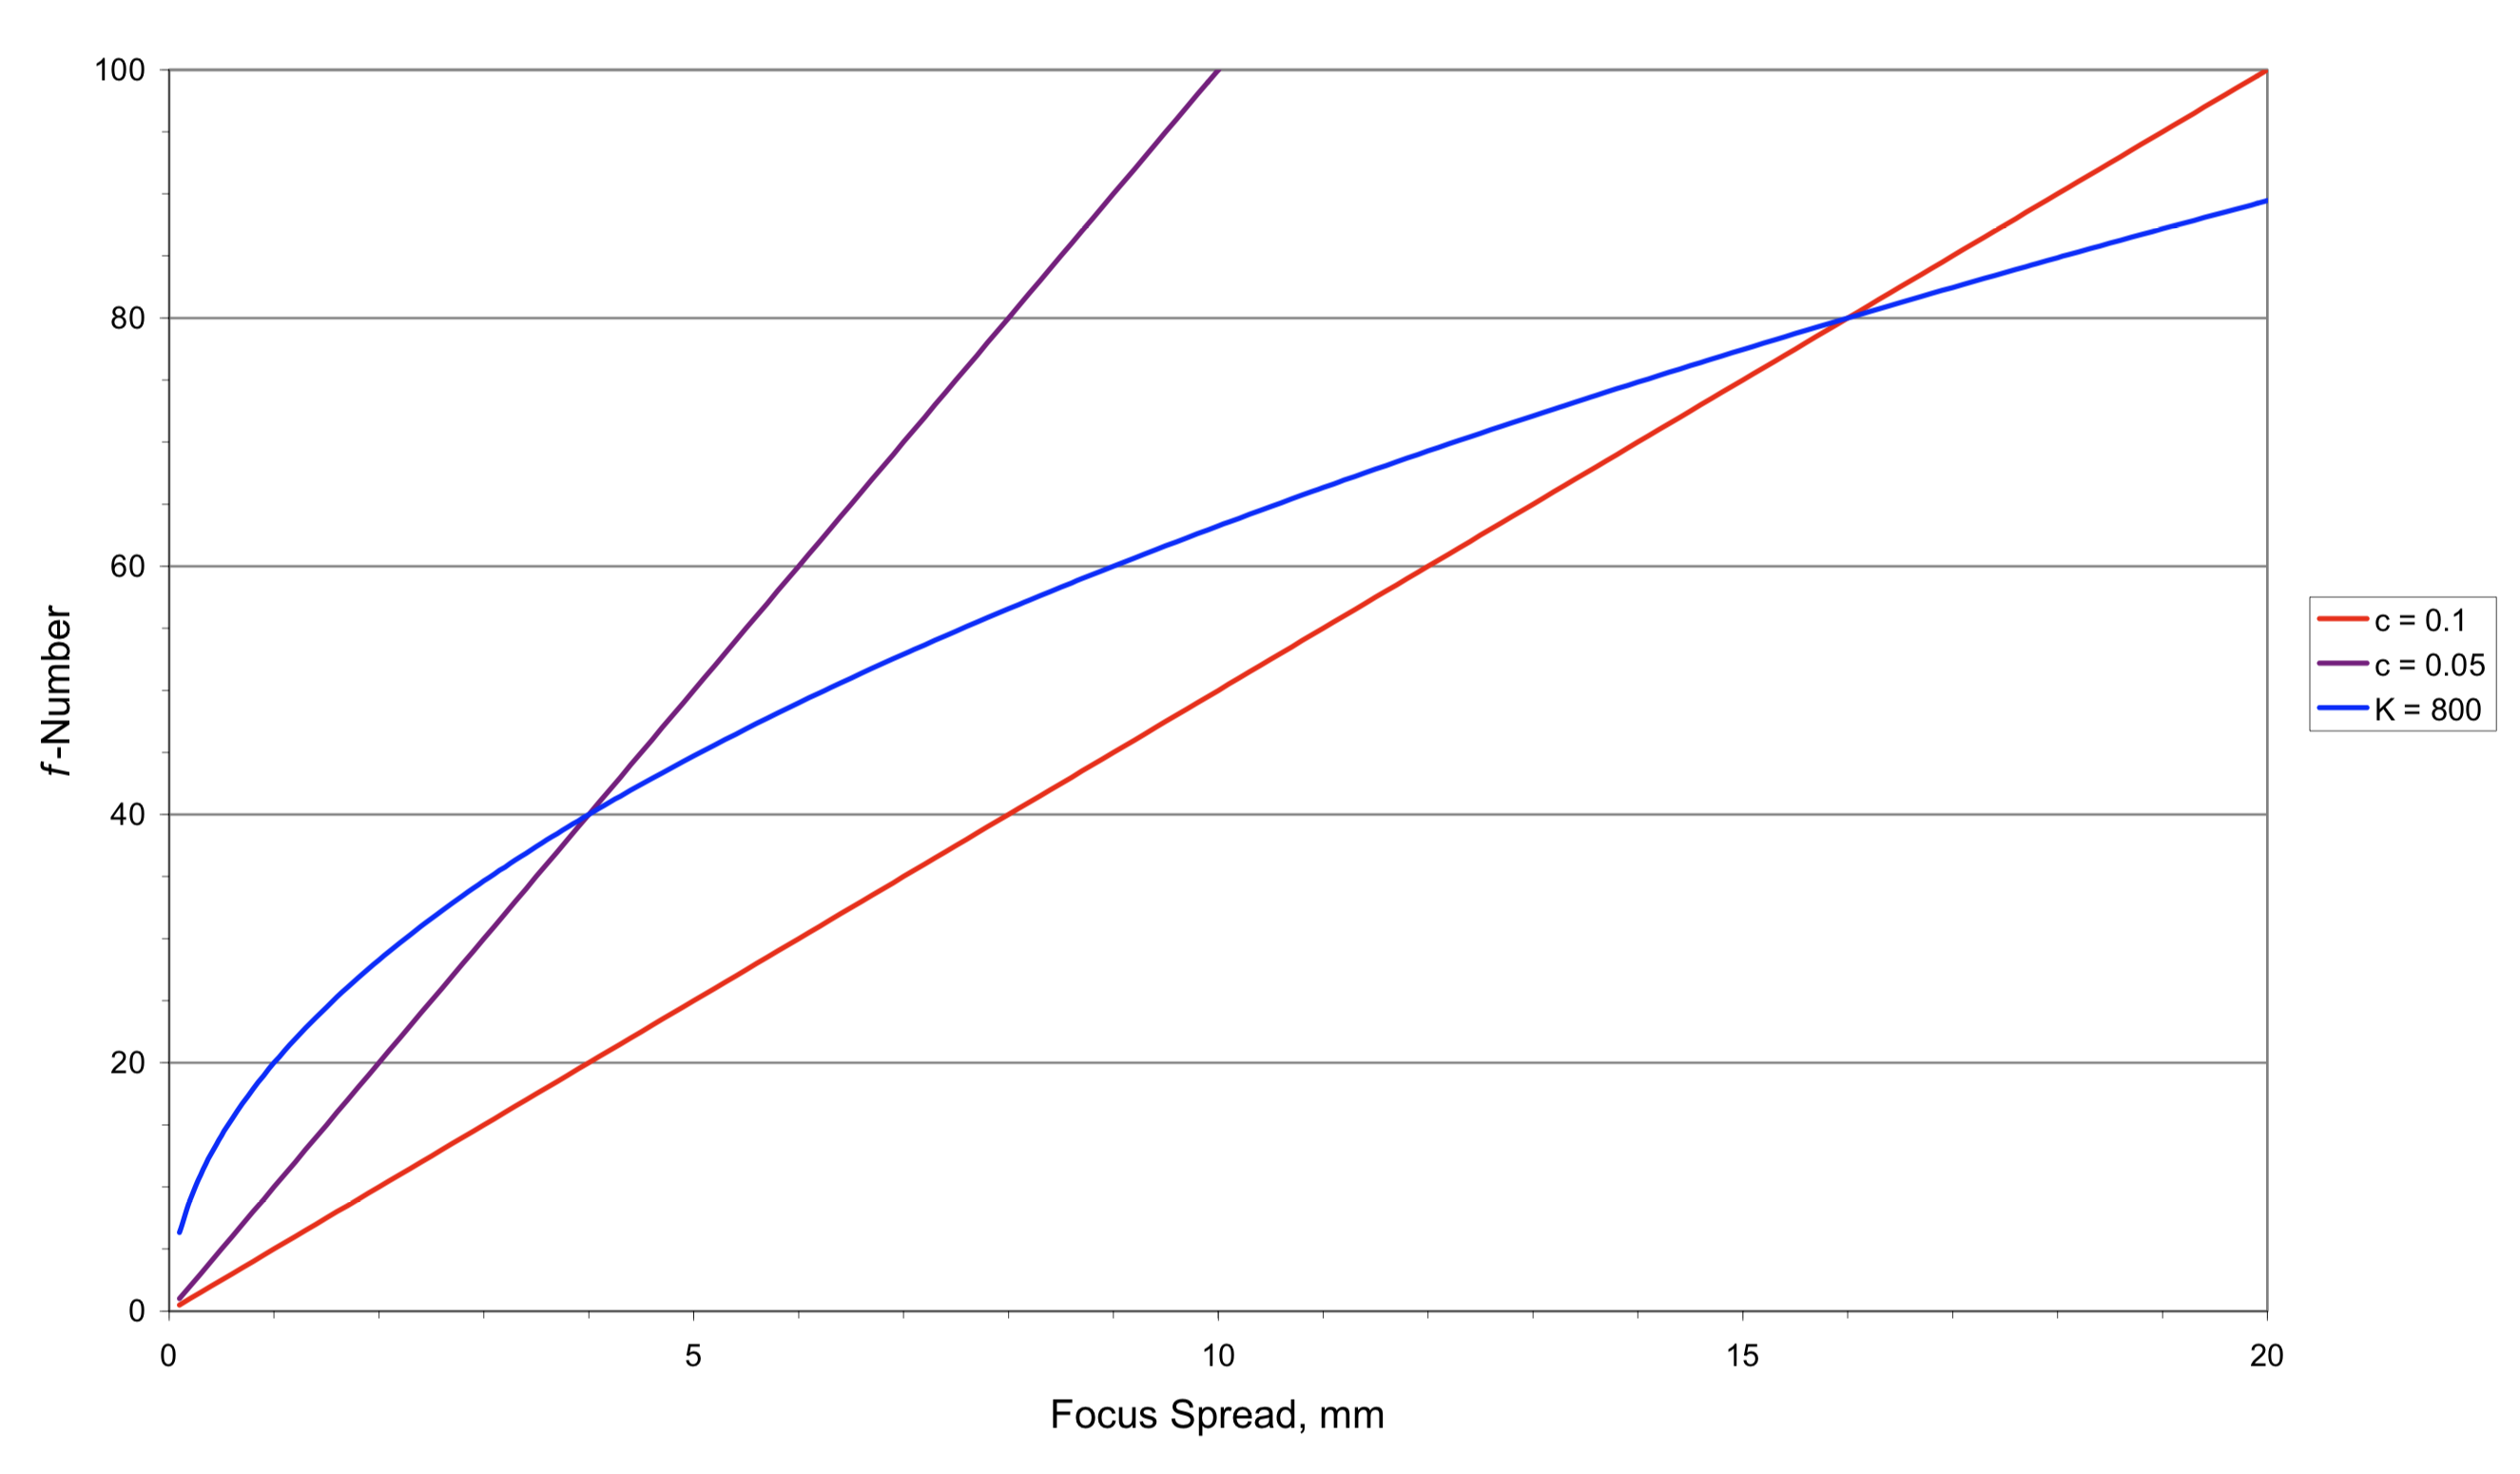
\includegraphics[width=\linewidth]{figure/fig_dofd_14} 
   \caption{$f$-number vs. Focus Spread: 0.1\,mm and 0.05\,mm CoCs and Hansma}
   \label{fig:fvsfspread}
\end{figure}
%% Figure 14. $f$-number vs. Focus Spread: 0.1\,mm and 0.05\,mm CoCs and Hansma
Figure~\ref{fig:fvsfspread} illustrates the effect of decreasing the CoC. With the standard 0.1\,mm CoC, the usable ranges of $f$-numbers are between the line marked ‘$c = 0.1$’ and the curve for the MTF-optimum method, marked ‘$K = 800$’. When the CoC is decreased to 0.05\,mm, the region of usable ranges becomes that between the steeper line and the MTF-optimum curve; the effect of the smaller CoC is to reach the optimum $f$-number at a smaller focus spread. From Eq.~\ref{eq:DvMTF}, if $K_λ = 800$, that limit now is reached at
\begin{equation}
Δv = 2c^2K_λ =2(0.05\,\mathrm{mm})^2×800\,\mathrm{mm}^{-1}=4\,\mathrm{mm}
\end{equation}

Once that point has been reached, there is no advantage to using an $f$-number greater than the optimum; at greater focus spreads, the blur spot is unavoidably larger than the nominal CoC. At small focus spreads, the smaller CoC will cause the minimum $f$-number to be closer to the optimum, giving somewhat greater sharpness.

The smaller CoC is somewhat of an illusion at large focus spreads, as illustrated in Figure~ref{figMTFvsf}. Increasing enlargement to 4$\times$ would imply that the critical spatial frequencies in the original image would be 4$\times$ those in the final image, or 8, 16, 24, and 32\,lp/mm. The effect is simply to add curves for 24 and 32\,lp/mm to Fig.~\ref{fig:MTFvsf10}; the resulting MTFs are quite low. The curves for 8 and 16\,lp/mm are unchanged, so that there really is no improvement in final-image sharpness. The best way to improve sharpness is to reduce the focus spread by employing camera movements whenever possible.
\begin{figure}[htbp] %  figure placement: here, top, bottom, or page
   \centering
   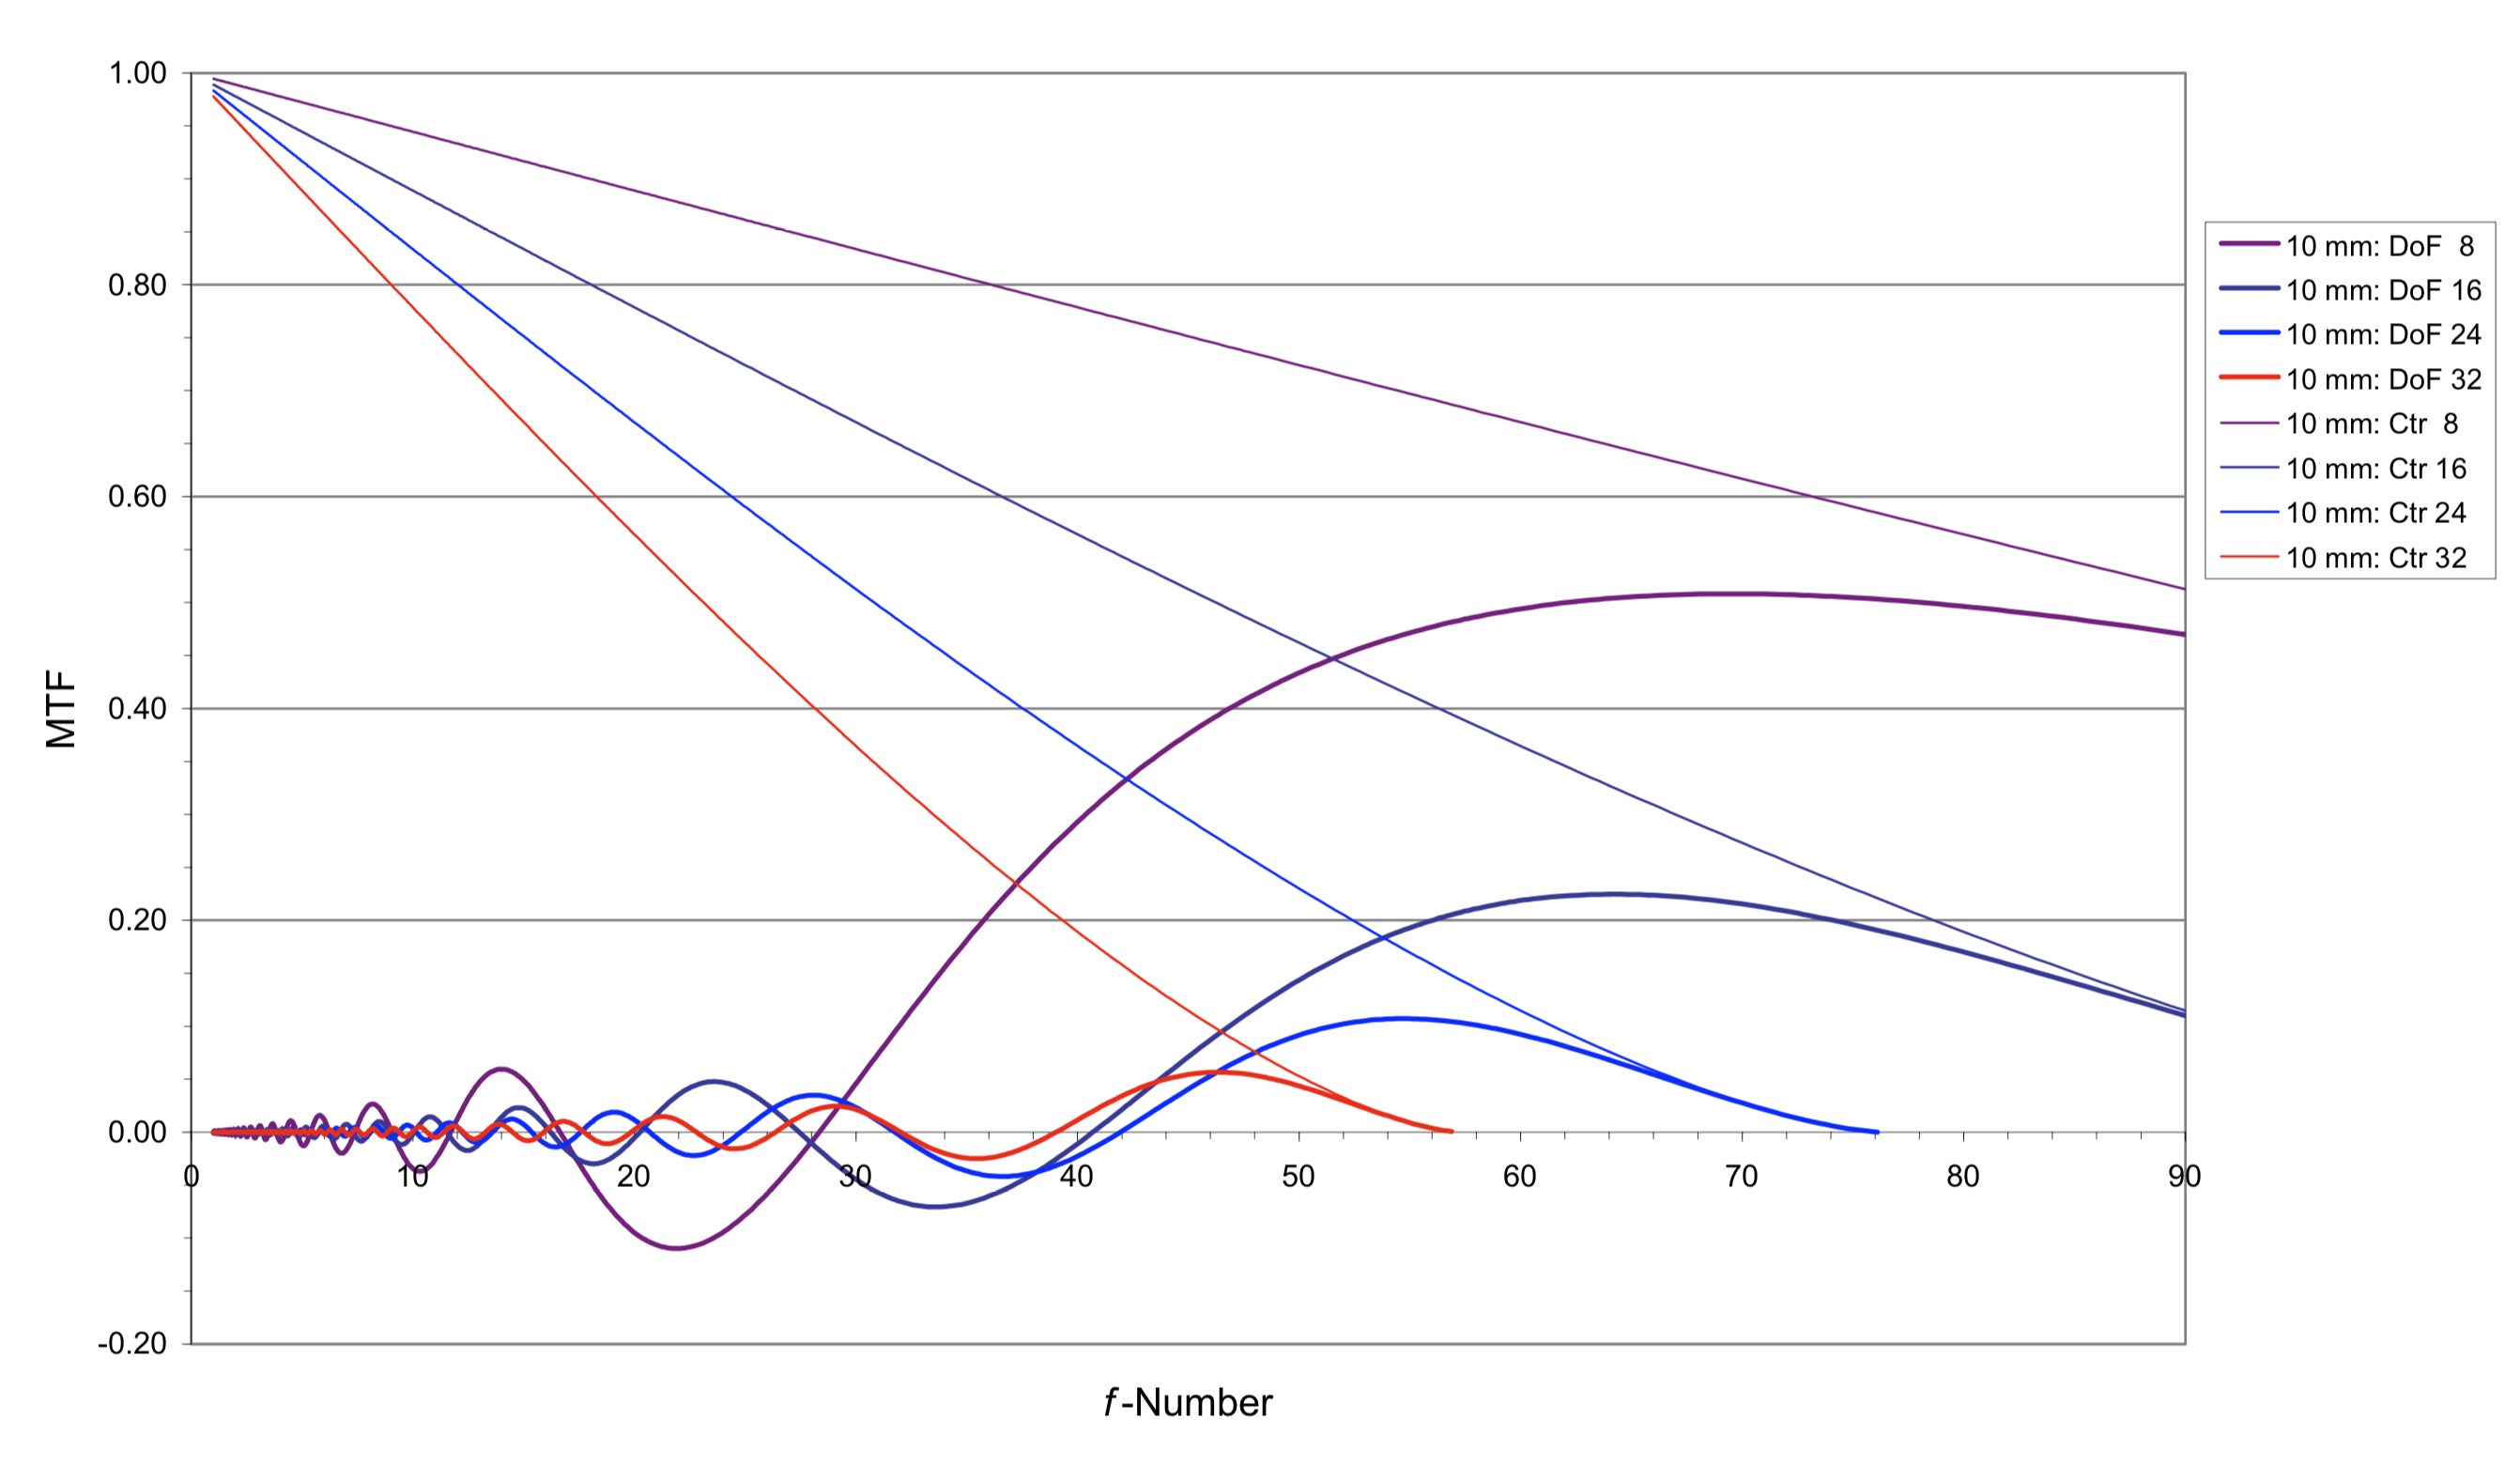
\includegraphics[width=\linewidth]{figure/fig_dofd_15} 
   \caption{MTF vs. $f$-Number: 4×5, 4× Enlargement, 10\,mm Focus Spread}
   \label{fig:MTFvsf2}
\end{figure}
%% Figure 15. MTF vs. $f$-Number: 4×5, 4× Enlargement, 10\,mm Focus Spread

When parameters are suitably scaled, the values of $a$ and $s$ in Eq. (117) do not change with camera format, so that results similar to those in Fig.~\ref{fig:MTFvsf3} and Fig.~\ref{fig:MTFvsf10} are obtained for any format. The appropriate spatial frequency is proportional to the image enlargement and hence to the format size:
\begin{equation}
   v \propto \frac1l
\end{equation}
For the blur spot,
\begin{equation}
k \propto \frac \delta N  \frac{Δv}{2N}
\end{equation}
For constant DoF, from Eqs. (34) and (74), within a suitably limited distance range, 
\begin{equation}
Δv \propto l^2 \quad ;
\end{equation}
from Eq. (76), within a suitably limited distance range, 
\begin{equation}
N\propto l\quad,
\end{equation}
so that
\begin{equation}
a = \pi v k = \pi v\frac{\Dv}{2N} \propto \frac{1}{l}\frac1l l^2 = 1
\end{equation}
%% a&πνk&πν Δv ∝11l2 &1
Similarly,
\begin{equation}
s=\lambda v N\propto \frac{l}{l}=1
\end{equation}
%s & λν N ∝ l & 1 l
%2N ll


For example, Fig.~\ref{fig:MTFvsf10} would be similar in appearance to a graph for the 35\,mm format with a focus spread of 0.625\,mm, spatial frequencies of 16, 32, 48, and 64\,lp/mm, and an $f$-number range of 1--22. This is illustrated in Figure~\ref{fig:MTFvsf35}.

\begin{figure}[htbp] %  figure placement: here, top, bottom, or page
   \centering
   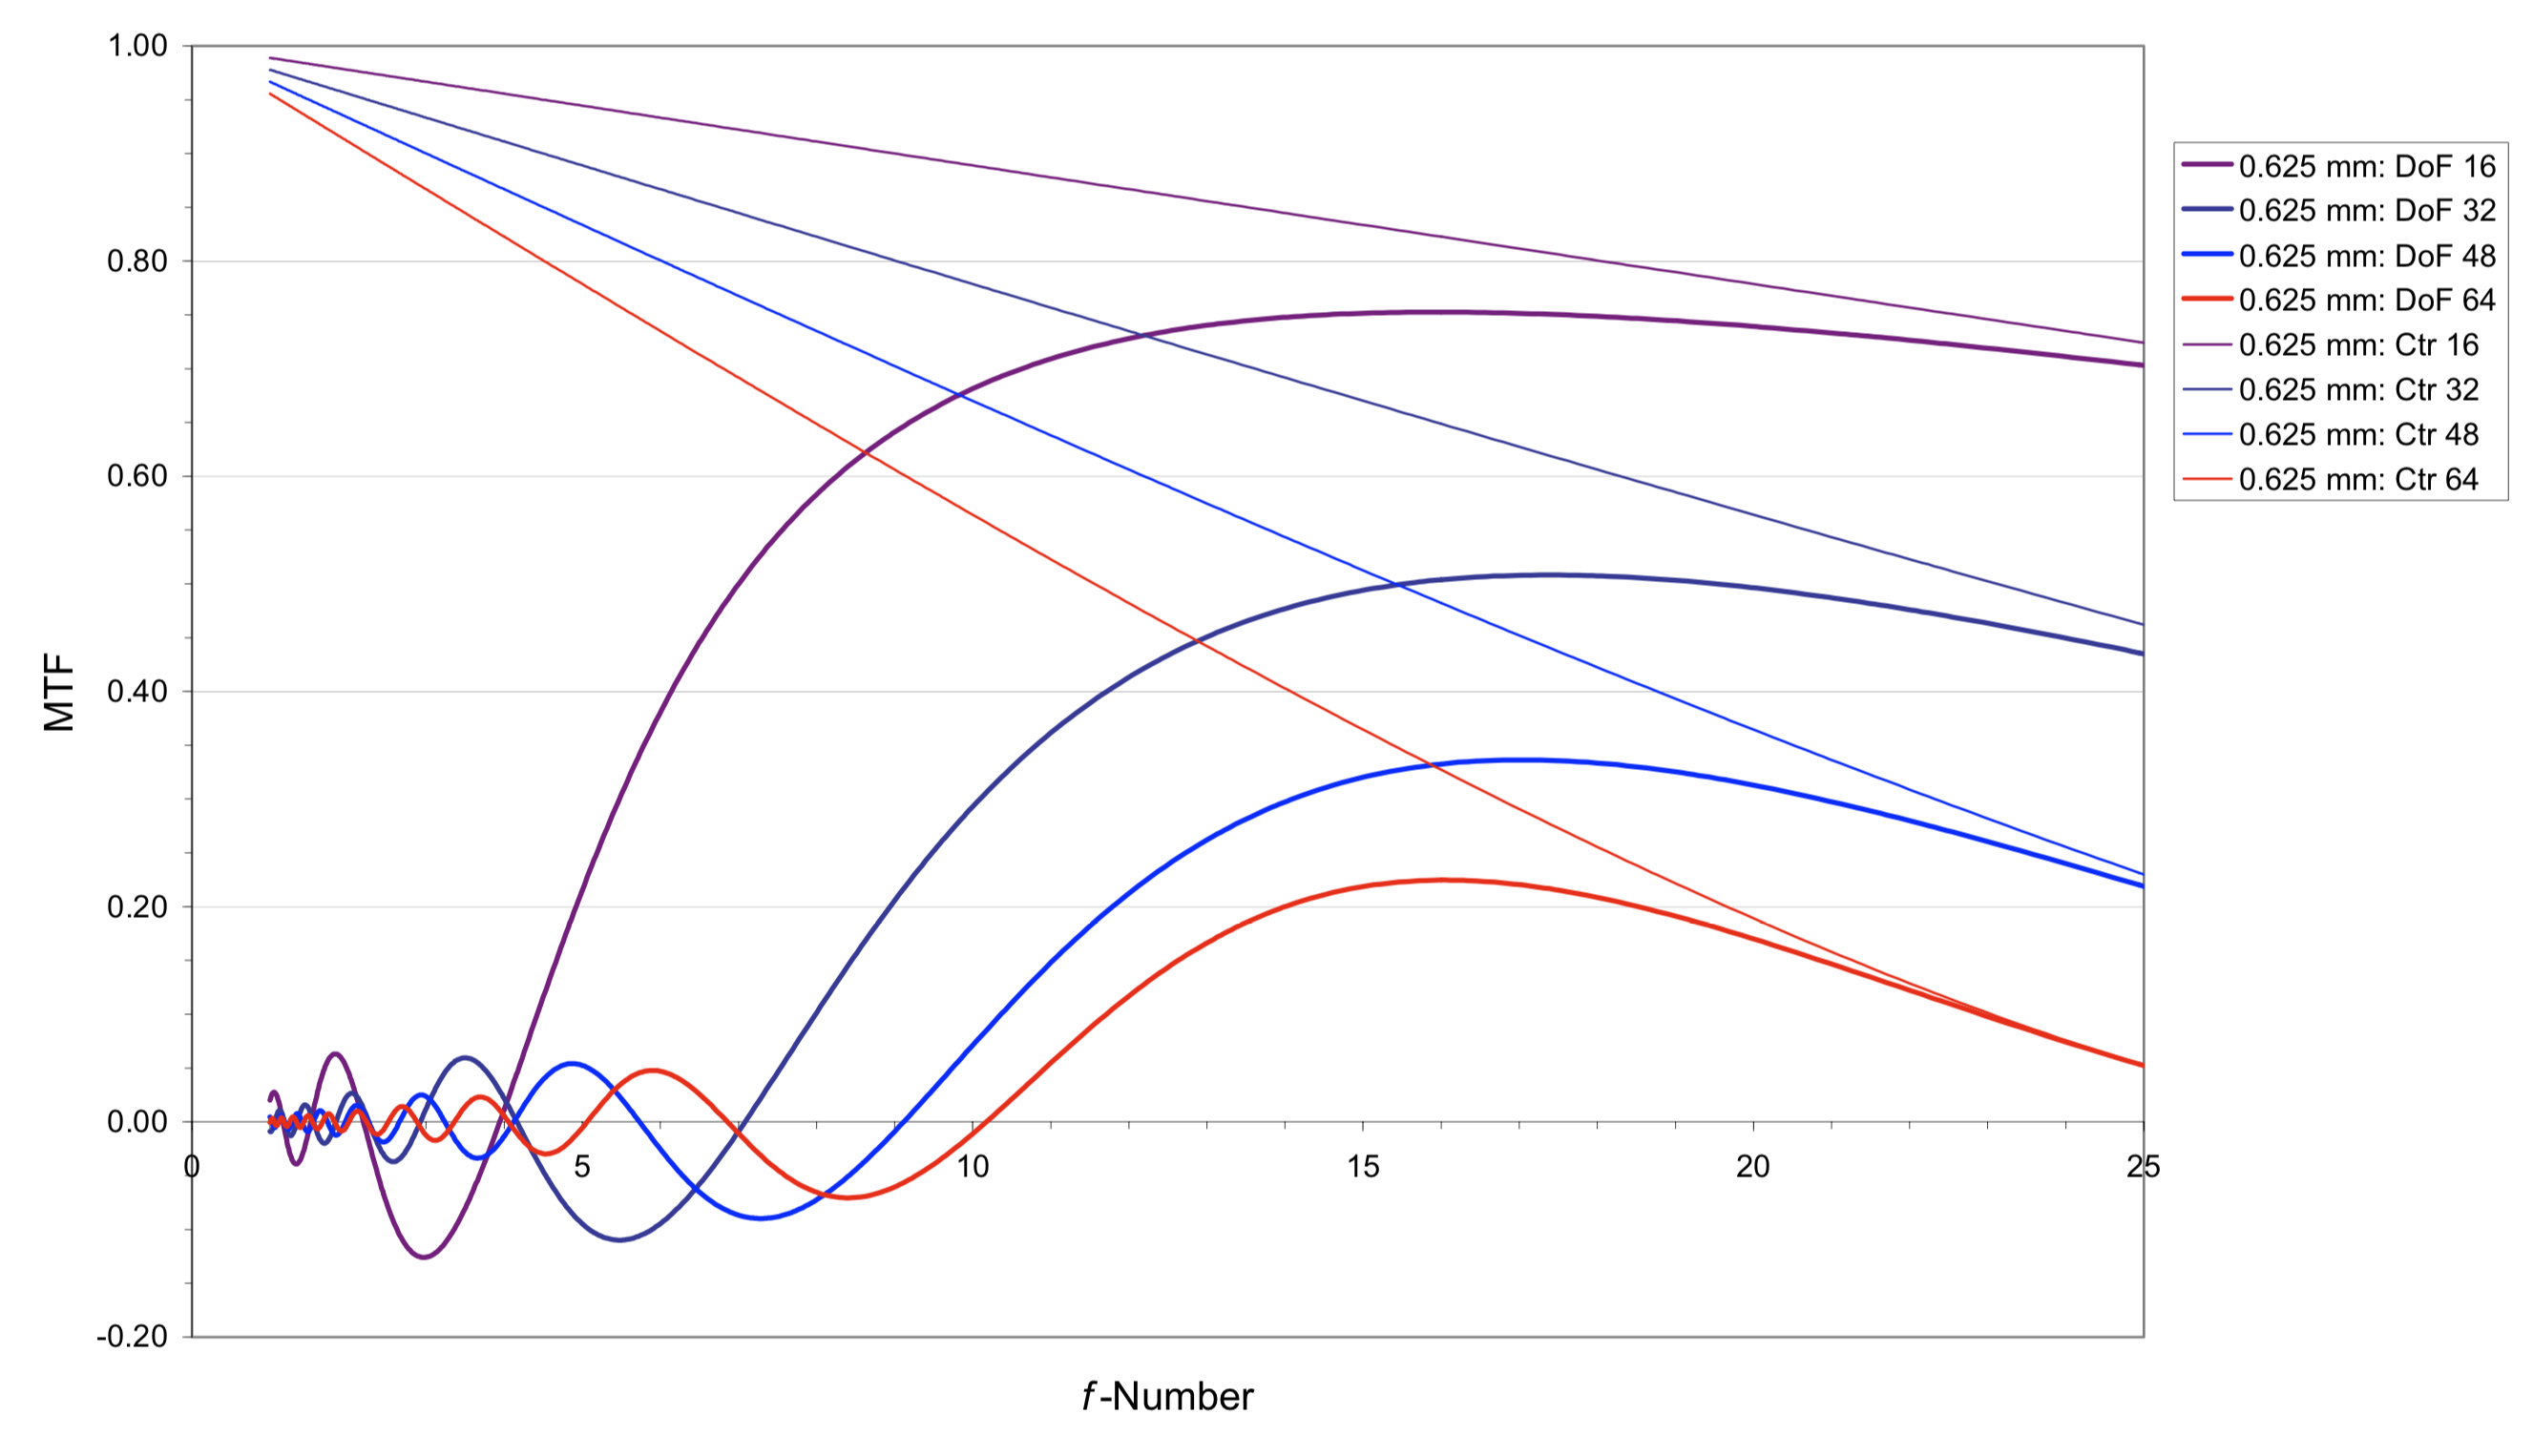
\includegraphics[width=\linewidth]{figure/fig_dofd_16} 
   \caption{MTF vs. $f$-Number: 35\,mm, 0.625\,mm Focus Spread}
   \label{fig:MTFvsf35}
\end{figure}
%%% Figure 16. MTF vs. $f$-Number: 35\,mm, 0.625\,mm Focus Spread

The spatial frequencies are greater than the commonly used 10, 20, 30, and 40\,lp/mm because enlargement is assumed to be 8$\times$ rather than 5$\times$.
It should be obvious that the optically determined sharpness of the final image essentially is independent of camera format. However, the image structure, especially film grain, contributes significantly to image degradation when small-format images are enlarged, so the larger formats still have significant advantages.

\section{Summary}

Practical control of DoF is achieved by setting the focus and $f$-number. The key variable for both settings is the focus spread $\Dv$, the difference $v_\mathrm{n} - v_\mathrm{f}$ between the near and far image distances. With a view camera, focus usually can be determined from Eq. (32), and the range of acceptable $f$-numbers can be determined from Eq. (121), so that
\begin{equation}
v = v_\mathrm{f} +\frac{\Dv}2
% v&vf +Δv 2
\end{equation}
and
\begin{equation}
\Dv \leq N \leq 20\sqrt{\Dv}
% Δv≤N≤20 Δv 2c
\end{equation}


The selection of an $f$-number within the acceptable range usually involves a tradeoff among sharpness at the DoF limits, sharpness at the plane of focus, and motion blur that might result from a longer exposure time. At very large focus spreads, the minimum $f$-number
deriving from the CoC may exceed the maximum dictated by diffraction; in such cases, the maximum $f$-number should be used.

On a manual-focus hand camera, the lens DoF scales usually implement Eqs. (32) and (39); a table of maximum $f$-numbers can be prepared using Eq. ~\ref{eq:Nmax2}. With autofocus lenses, however, there may be no easy means of controlling DoF.

Close-focusing ``macro" lenses for small-format cameras usually are asymmetrical and often are internal focusing. When such lenses are used at high magnification, the DoF may differ significantly from that given by formulae for symmetrical unit-focusing lenses. In most cases, the parameters required for DoF calculations with such lenses are not known, so the lens manufacturer’s DoF data usually are the best source of information. With most other lenses, even if not symmetrical or unit focusing, the symmetrical-lens formulae are more than adequate.

The standard CoCs used in DoF calculations assume certain conditions of image enlargement and viewing. If the actual conditions differ substantially from those assumed, especially if the photographer plans to examine large images at close distances, sharpness may not be as great as desired. To some extent, the CoC can be adjusted to suit the different conditions, but diffraction imposes limits on how much sharpness can be improved by reducing the CoC. When great DoF is required, it simply may not be possible to have everything as sharp as desired.

\section{Definitions of Quantity Symbols}
%\begin{table}[htp]
%\caption{default}
\begin{center}
{\small
\begin{tabular}{r@{~=~}l}
$\delta$ & Lens defocus     \\
$\lambda$ & Wavelength of light     \\
$v$ & Spatial frequency of object or image pattern     \\
$v_0$ & Cutoff spatial frequency for which MTF = 0      \\
$c$ & Acceptable circle of confusion     \\
$c_\mathrm{f}$ & Acceptable circle of confusion for objects at far limit of DoF     \\
$c_\mathrm{n}$ & Acceptable circle of confusion for objects at near limit of
        DoF     \\
$c_\mathrm{mkd}$ & Circle of confusion used to determine lens DoF scale     \\
$c_\mathrm{T}$ & Total acceptable circle of confusion for defocus and
        diffraction     \\
$D$ & Diameter of lens entrance pupil      \\
$d$ & Diameter of lens exit pupil     \\
$f$ & Lens focal length     \\
$K_\lambda$ & Constant relating diffraction blur spot size to
              wavelength of light     \\
$k$ & Diameter of blur spot for defocused point at object distance
      $u_\mathrm{d}$     \\
$k_\mathrm{def}$ & Diameter of defocus blur spot     \\
$k_\mathrm{diff}$ & Diameter of diffraction blur spot     \\
$k_\mathrm{r}$ & “Relative blur” of defocused object     \\
$L_\mathrm{max}$ & Maximum luminance of test pattern or its image      \\
$L_\mathrm{min}$ & Minimum luminance of test pattern or its image     \\
$l$ & Camera format characteristic dimension\\
$m$ & Image magnification at  focused distance     \\
$m_\mathrm{d}$ & Image magnification of object at distance $x_\mathrm{d}$ from plane of
     focus      \\
$m_\mathrm{h}$ & Image magnification at hyperfocal distance     \\
$N$ & Relative aperture ($f$-number) of lens, $f/D$     \\
$N_\mathrm{ap}$ & Approximate $f$-number for large object distance     \\
$N_\mathrm{mkd}$ & Marked $f$-number on lens     \\
$N_\mathrm{opt}$ & Optimum $f$-number determined from MTF or Hansma’s method     \\
$p$ & Pupillary magnification of lens, $d/D$     \\
$S$ & Diameter of smallest object feature to be resolved      \\
$s_\mathrm{ep}$ & Distance of entrance pupil behind object vertex     \\
$s_\mathrm{H}$ & Distance of object principal plane behind object vertex      \\
$s'_\mathrm{ap}$ & Distance of exit pupil behind image vertex     \\
$s'_\mathrm{H'}$ & Distance of image principal plane behind image vertex     \\
$x_\mathrm{ep}$& Distance of entrance pupil behind object principal plane      \\
$x'_\mathrm{ap}$ & Distance of exit pupil behind image principal plane     \\
$u$ & Distance from object to object principal plane     \\
$u_\mathrm{d}$ & Distance from defocused object to object principal plane     \\
$u_\mathrm{f}$ & Far limit of depth of field     \\
$u_\mathrm{h}$ & Hyperfocal distance, for which $u_\mathrm{f} = \infty$      \\
$u_\mathrm{n}$ & Near limit of depth of field     \\
$v$ & Distance from film plane to image principal plane      \\
$v_\mathrm{ap}$ & Approximate image distance for small focus spread     \\
$v_\mathrm{d}$ & Image distance for defocused object at object distance $u_\mathrm{d}$      \\
$v_\mathrm{f}$ & Image distance for far limit of depth of field     \\
$v_\mathrm{h}$ & Image distance for hyperfocal distance $_\mathrm{h}$     \\
$v_\mathrm{n}$ & Image distance for near limit of depth of field      \\
$\Dv$ & Focus spread $v_\mathrm{n} - v_\mathrm{f}$     \\
$x_\mathrm{d}$ & Distance of defocused object from plane of focus      \\
$x_\mathrm{h}$ & Object-to-image hyperfocal distance     \\
\end{tabular}
}
\end{center}
%\label{default}
%\end{table}%

\section{References}

Campbell, F.W., and Green, D.G. 1965. ``Optical and Retinal Factors Affecting Visual Resolution,'' J. Physiol. 181:576–-593.\\
Englander, Joe. 1994. Apparent Depth of Field: Practical Use in Landscape Photography. Available in PDF at \url{http://www.englander-workshops.com/documents/depth.pdf}.\\
Evens, Leonard. 2003. Some Thoughts on View Camera Calculations. Available in PDF at \url{math.northwestern.edu/~len/photos/pages/dof_essay.pdf}.\\
Hansma, Paul K. 1996. ``View Camera Focusing in Practice,'' Photo Techniques, March/April 1996, 54–57. Available in PDF at \url{http://www.largeformatphotography.info/}.\\
Hayashi, Masayoshi. Making a DOF calculator for your camera. \url{http://www.largeformatphotography.info/dofknob/}.\\
Hopkins, H. H. 1955. ``The frequency response of a defocused optical system,'' Proceedings of the Royal Society A, 231:91--103.\\
Jacobson, David M. 1992. Lens Tutorial. \url{http://www.photo.net/photo/optics/lensTutorial}.\\
Jacobson, Ralph E. 2000. ``Fundamentals of light and vision.'' In The Manual of Photography, 9th ed. Oxford: Focal Press.\\
Merklinger, Harold M. 1992. The INs and OUTs of FOCUS, v. 1.0.3. Bedford, Nova Scotia: Seaboard Printing Limited. Version 1.03e available in PDF at \url{http://www.trenholm.org/hmmerk/}.\\
Ray, Sidney F. 2002. Applied Photographic Optics, 3rd ed. Oxford: Focal Press.\\
Van Walree, Paul. 2002. Depth of Field. \url{www.vanwalree.com/optics/dof.html}.\\
Williams, Charles S., and Becklund, Orville. 1989. A. Introduction to the Optical Transfer Function. NewYork: Wiley. Reprinted 2002, Bellingham, WA: SPIE Press.\\
Williams, John B. 1990. Image Clarity: High-Resolution Photography. Boston: Focal Press. 

\subsection{Additional Reading}
Smith, Warren J. ``Image Formation: Geometrical and Physical Optics.'' In Handbook of Optics, ed. Walter G. Driscoll, 2-26 through 2-35. New York: McGraw-Hill, 1978.\\
Wheeler, Robert E. 1999. ``Notes on View Camera Geometry.'' Available in PDF at \url{http://www.bobwheeler.com/}.

\appendix
\section{Erratum}

Eq. (44), which gives the magnification of a defocused object, is
inapplicable to an asymmetrical lens, so Eq. (96), which gives the
``relative blur'' of a defocused object with an asymmetrical lens, is incorrect.
For an asymmetrical lens, the object conjugate $u_\mathrm{p}$ is the distance from the object point to the entrance pupil (Ray 2002, 125):
\begin{equation}
u_\mathrm{p} = u + x_\mathrm{ep}\quad .
\end{equation}

From Eq. (81),
\begin{equation}
x_\mathrm{ep} =\left(\frac{1}{p}-1\right)f\quad,
\end{equation}
so that
\begin{eqnarray}
u_\mathrm{p} &=&(1+1/m)f+ (1/p - 1)f\\
& = &\left(\frac{1}{m} + \frac{1}{p}\right)f.
\end{eqnarray}
The image conjugate distance is
\begin{equation}
v_\mathrm{p} = mu_\mathrm{p}=\left(1+ \frac{m}{p}\right)f\quad.
\end{equation}
The magnification $m_\mathrm{d}$ of an object at a distance $u_\mathrm{d}$ from the front principal plane is
\begin{equation}
  m_\mathrm{d}=\frac{v_\mathrm{p}}{u_\mathrm{d} + x_\mathrm{ep}} = \frac{(1+\frac{m}{p})f}{ u_\mathrm{d} + x_\mathrm{ep}} = \frac{(1+\frac{m}{p})f}{u_\mathrm{d} +(\frac{1}{p}-1)f} \quad.
\end{equation}
From Eq. (95), the diameter of the blur spot for a defocused point
object at distance $u_\mathrm{d}$ is
\begin{equation}
  \label{eq:a6}
  k = \frac{pfm}N\frac{|u_\mathrm{d}-u|}{u_\mathrm{d}+(u_\mathrm{d}-f)(p-1)}\quad;  
\end{equation}
the ``relative blur''  is then
\begin{equation}
  \label{eq:a7}
  k_\mathrm{r} = \frac k{m_\mathrm{d}} = \frac{pfm}N\frac{|u_\mathrm{d}-u|}{u_\mathrm{d}+(u_\mathrm{d}-f)(p-1)}\frac{u_\mathrm{d}p+(1-p)f}{(m+p)f}
  \quad.
\end{equation}
Expanding, rearranging, and factoring the numerator of the third
fraction gives
\begin{equation}
  \label{eq:a8}
   k_\mathrm{r} = \frac{mp}N\frac{|u_\mathrm{d}-u|}{u_\mathrm{d}+(u_\mathrm{d}-f)(p-1)}\frac{u_\mathrm{d}+(u_\mathrm{d}-f)(p-1)}{m+p}\quad;
 \end{equation}
 cancelling terms and rearranging gives
 \begin{equation}
   \label{eq:a9}
   k_\mathrm{r} = \frac m{1+m/p}\frac{|u_\mathrm{d}-u|}N\quad,
 \end{equation}
the same as for a symmetrical lens except that the denominator of the first fraction is $1 + m/p$ rather than $1 + m$.
\end{document}  